\section{Modelling}\label{sec:ggtt_modelling}
To extract the final results in \cref{sec:ggtt_results}, a statistical model for the data, and a corresponding likelihood function is constructed. There is a single parameter of interest, $\mu$, which is the cross section for the di-Higgs signal process in \fb, and the primary observable is chosen as the diphoton mass, \mgg, in the analysis categories defined in \cref{sec:cat_optim}. The likelihood function is constructed as described in \cref{chap:stats} for a parametric shape analysis and the inputs to this construction, for every process, and for every analysis category, are:
\begin{itemize}
  \item $\lambda(\vec{\mu},\vec{\nu})$ --- the expected number of events
  \item $f(\mgg;\mu,\vec{\Psi})$ --- the probability density function (pdf) for the diphoton mass
\end{itemize}
which can be optionally factorized into nominal values and components that encode the impact of systematic uncertainties (\cref{sec:stats_systematics}), in which case the inputs are:
\begin{itemize}
  \item $g(\vec{\mu})$ --- the nominal expected number of events (\cref{eq:lambda_definition})
  \item $\vec{\hat{\Psi}}$ --- the nominal shape parameters for $f(\mgg;\mu,\vec{\Psi})$ 
  \item $(\kup)_k$ and $(\kdown)_k$ --- parameters describing the impact of the nuisance parameter $\nu_k$ on $\lambda(\mu,\vec{\nu})$ (\cref{eq:kappa_definition})
  \item $\alpha_{ik}$ --- parameters describing the impact of the nuisance parameter $\nu_k$ on $\Psi_i$ (\cref{eq:alpha_definition}).
\end{itemize}
This section describes the determination of these inputs, where the methods used depend on the type of process. \cref{sec:h_hh_modelling} describes the MC-driven methods used for the signal process and single Higgs background process. \cref{sec:non_res_bkg_modelling,sec:dy_bkg_modelling} describe the data-driven methods used for the nonresonant background, and the DY background, respectively.

\subsection{Single and Di-Higgs Production}\label{sec:h_hh_modelling}

At the nominal mass points, the single Higgs and di-Higgs processes are modelled using MC simulation, and the methods used are identical. This section begins by describing these methods, before moving onto the models at the intermediate mass points, which for the di-Higgs processes, are determined using interpolation methods.

For the signal and single Higgs processes, models are created per data-taking year (2016, 2017 and 2018). This is not strictly necessary since the final fit to data is performed with all years combined, but is done for practical reasons because the systematic uncertainties are derived per year. 

\subsubsection{Single Higgs and Nominal Mass Points}\label{sec:single_dihiggs_modelling}
For the di-Higgs process, the nominal expected number of events in analysis category, $c$, for data-taking year, $y$, is parameterized as:
\begin{equation}
  g_{cy}(\mu) = \mu \cdot \sigma \cdot \epsilon_{cy} \cdot (\Lint)_y
\end{equation}
where $(\Lint)_y$ is the integrated luminosity in \fbinv for data-taking year, $y$, $\epsilon_{cy}$ is an efficiency which is the fraction of events that pass the selection criteria in category $c$ for a particular year, relative to all produced events, and $\sigma$ is set to $\sigma=1$ so that $\mu$ represents the cross section for the process in \fb where the cross section includes the branching fractions of the Higgs boson decays. Similarly, for a single Higgs process, $p$, $g_{pc}$ is parameterized as:
\begin{equation}
  g_{pc} = \sigma_p \cdot \BR_\Hgg \cdot \epsilon_{pcy} \cdot (\Lint)_y
\end{equation}
where $\mu$ is now omitted and the values of $\sigma_p$ and $\BR_\Hgg$ are taken from the LHC Higgs Cross Section Working Group~\cite{LHCHiggsCrossSectionWorkingGroup:2016ypw}, which are listed in \cref{tab:higgs_xs,tab:higgs_brs}. For the single and di-Higgs processes, the efficiencies, $\epsilon$, are calculated using MC simulation.

The nominal pdfs, $f_{pcy}(\mgg;\mu,\vec{\hat{\Psi}})$, are determined by $\chi^2$ fits of a Double Crystal Ball (DCB) function to MC events. A DCB consists of a Gaussian core which switches to a power law function on the left and another power law function on the right of the distribution:
\begin{equation}
    f(\mgg; \hat{m}_{\gamma\gamma}, \sigma, \beta_l, m_l, \beta_r, m_r) = \begin{cases}
      \exp(-x^2/2) & \text{for } -\beta_l < x < \beta_r \\
      A(\beta_l, m_l) \cdot (B(\beta_l, m_l) - x)^{-m_l} & \text{for } x < -\beta_l \\
      A(\beta_r, m_r) \cdot (B(\beta_r, m_r) + x)^{-m_r} & \text{for } x > \beta_r
    \end{cases}\label{eq:DCB}
\end{equation}
where
\begin{gather}
    x = \frac{\mgg - \hat{m}_{\gamma\gamma}}{\sigma} \\
    A(\beta, m) = \left(\frac{m}{|\beta|}\right)^m \cdot \exp\left(-\frac{|\beta|^2}{2} \right) \\
    B = \frac{m}{\beta} - |\beta|
\end{gather}
The $\chi^2$ fits are performed in 50 bins of the \mgg distribution in a 25\GeV window centred at 125\GeV for the single Higgs processes, and the di-Higgs processes for the \XHH searches and the \XYttHgg searches. In the \XYggHtt searches, the window is centred at \mY, and the size of the window is scaled linearly with \mY to account for the increasing width of the \mgg distribution. Examples of these fits are shown in \cref{fig:dcb_fits}. In general, the DCB is a good model for the \mgg distribution as indicated by values of $\chi^2$ which are approximately equal to the degrees of freedom.

\begin{figure}
  \centering
  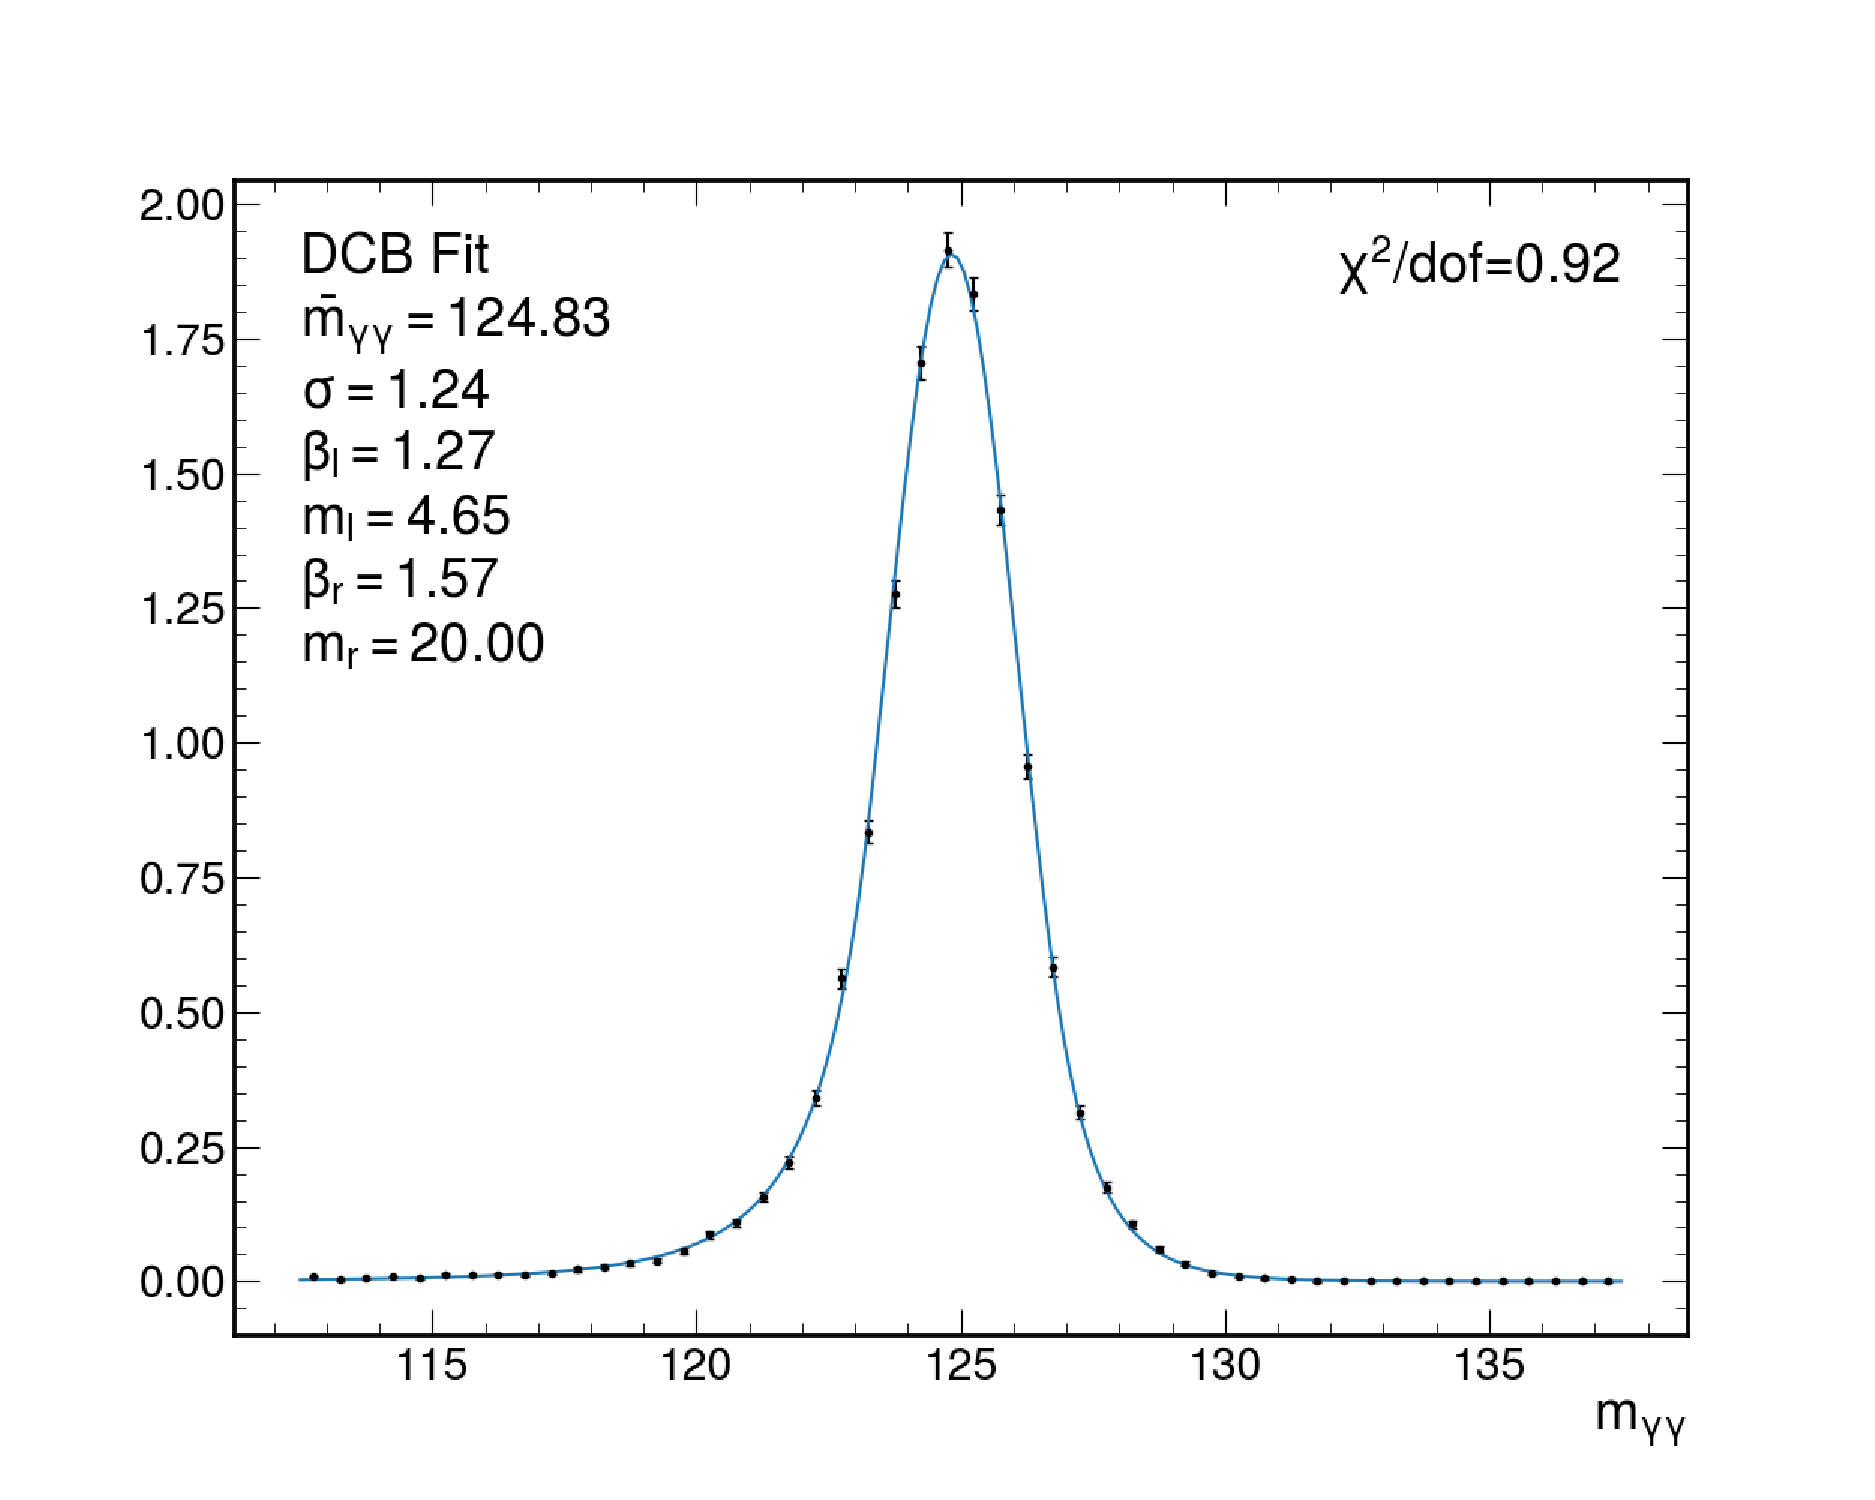
\includegraphics[width=0.49\textwidth]{Figures/Dihiggs/signal/tautau_mx_600_my_90.pdf}
  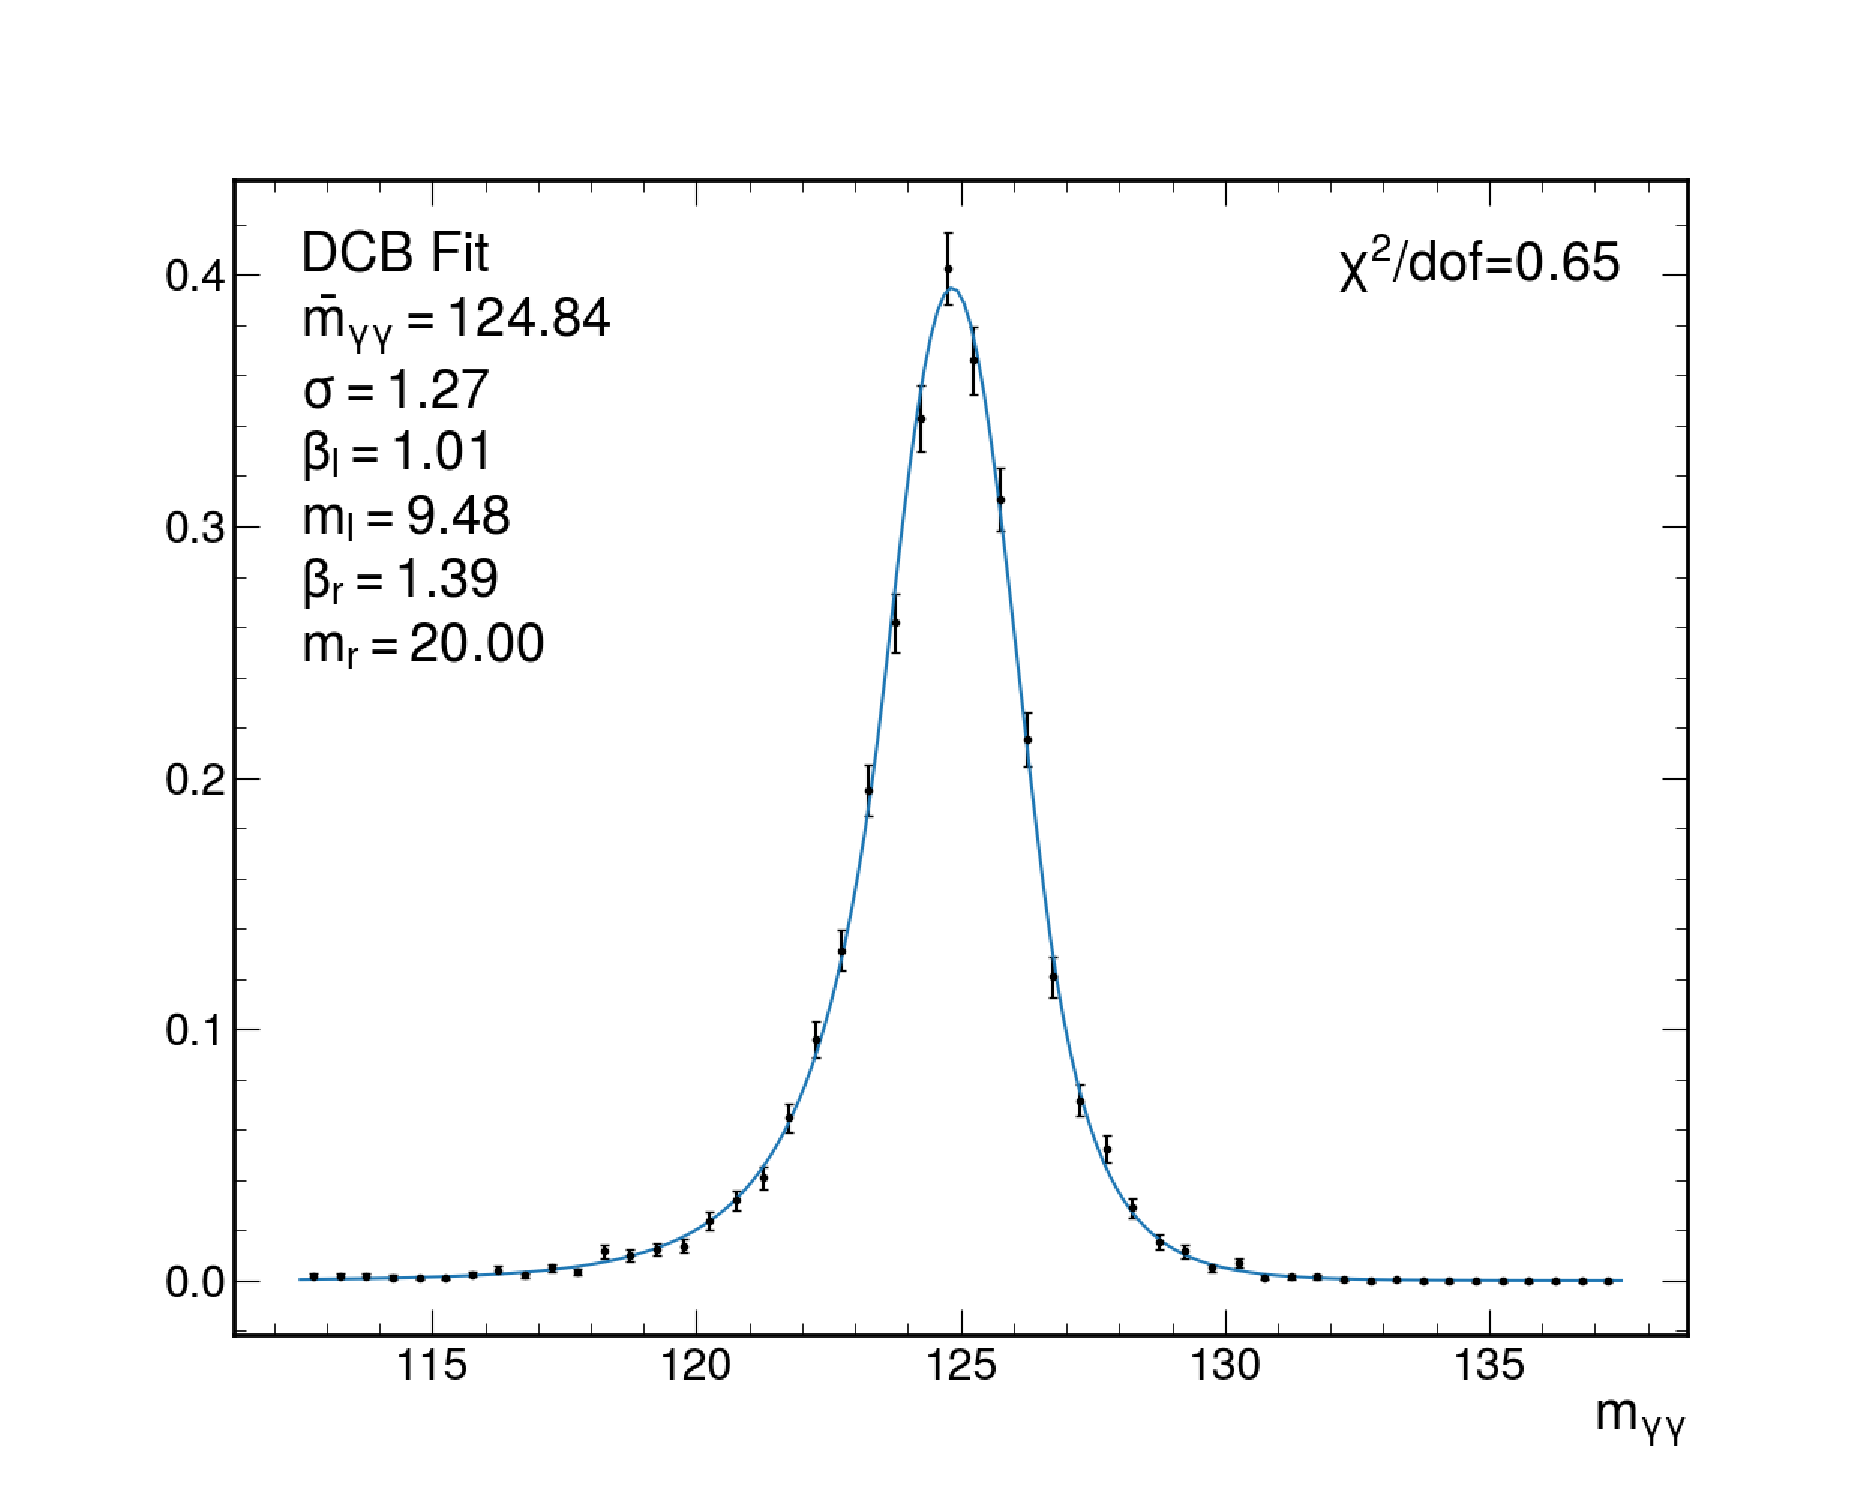
\includegraphics[width=0.49\textwidth]{Figures/Dihiggs/signal/tautau_mx_300_my_70.pdf} \\
  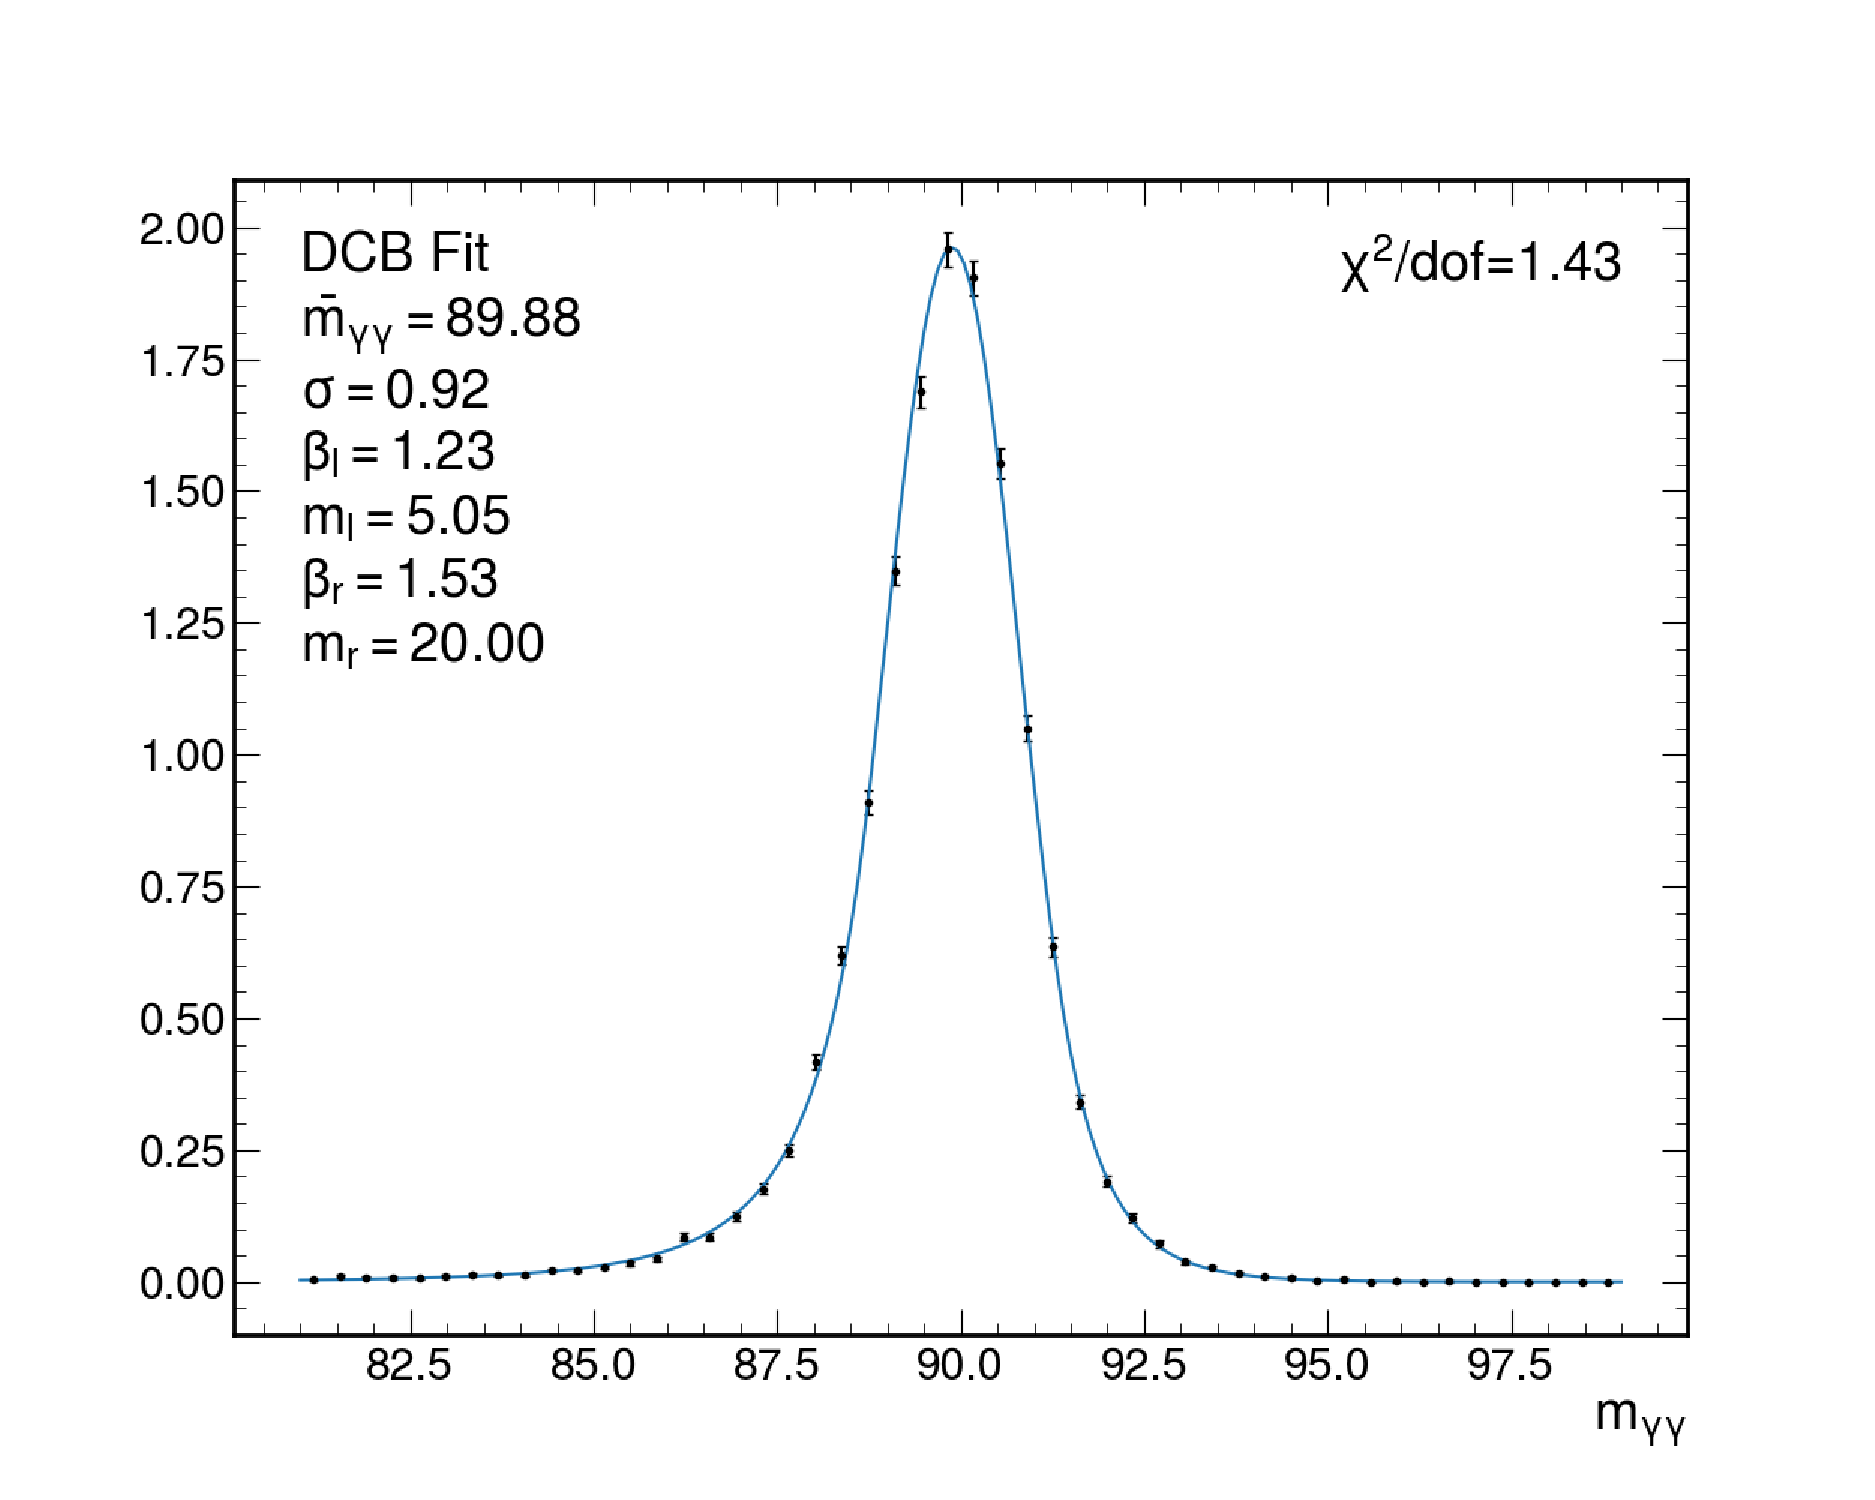
\includegraphics[width=0.49\textwidth]{Figures/Dihiggs/signal/low_mass_mx_600_my_90.pdf}
  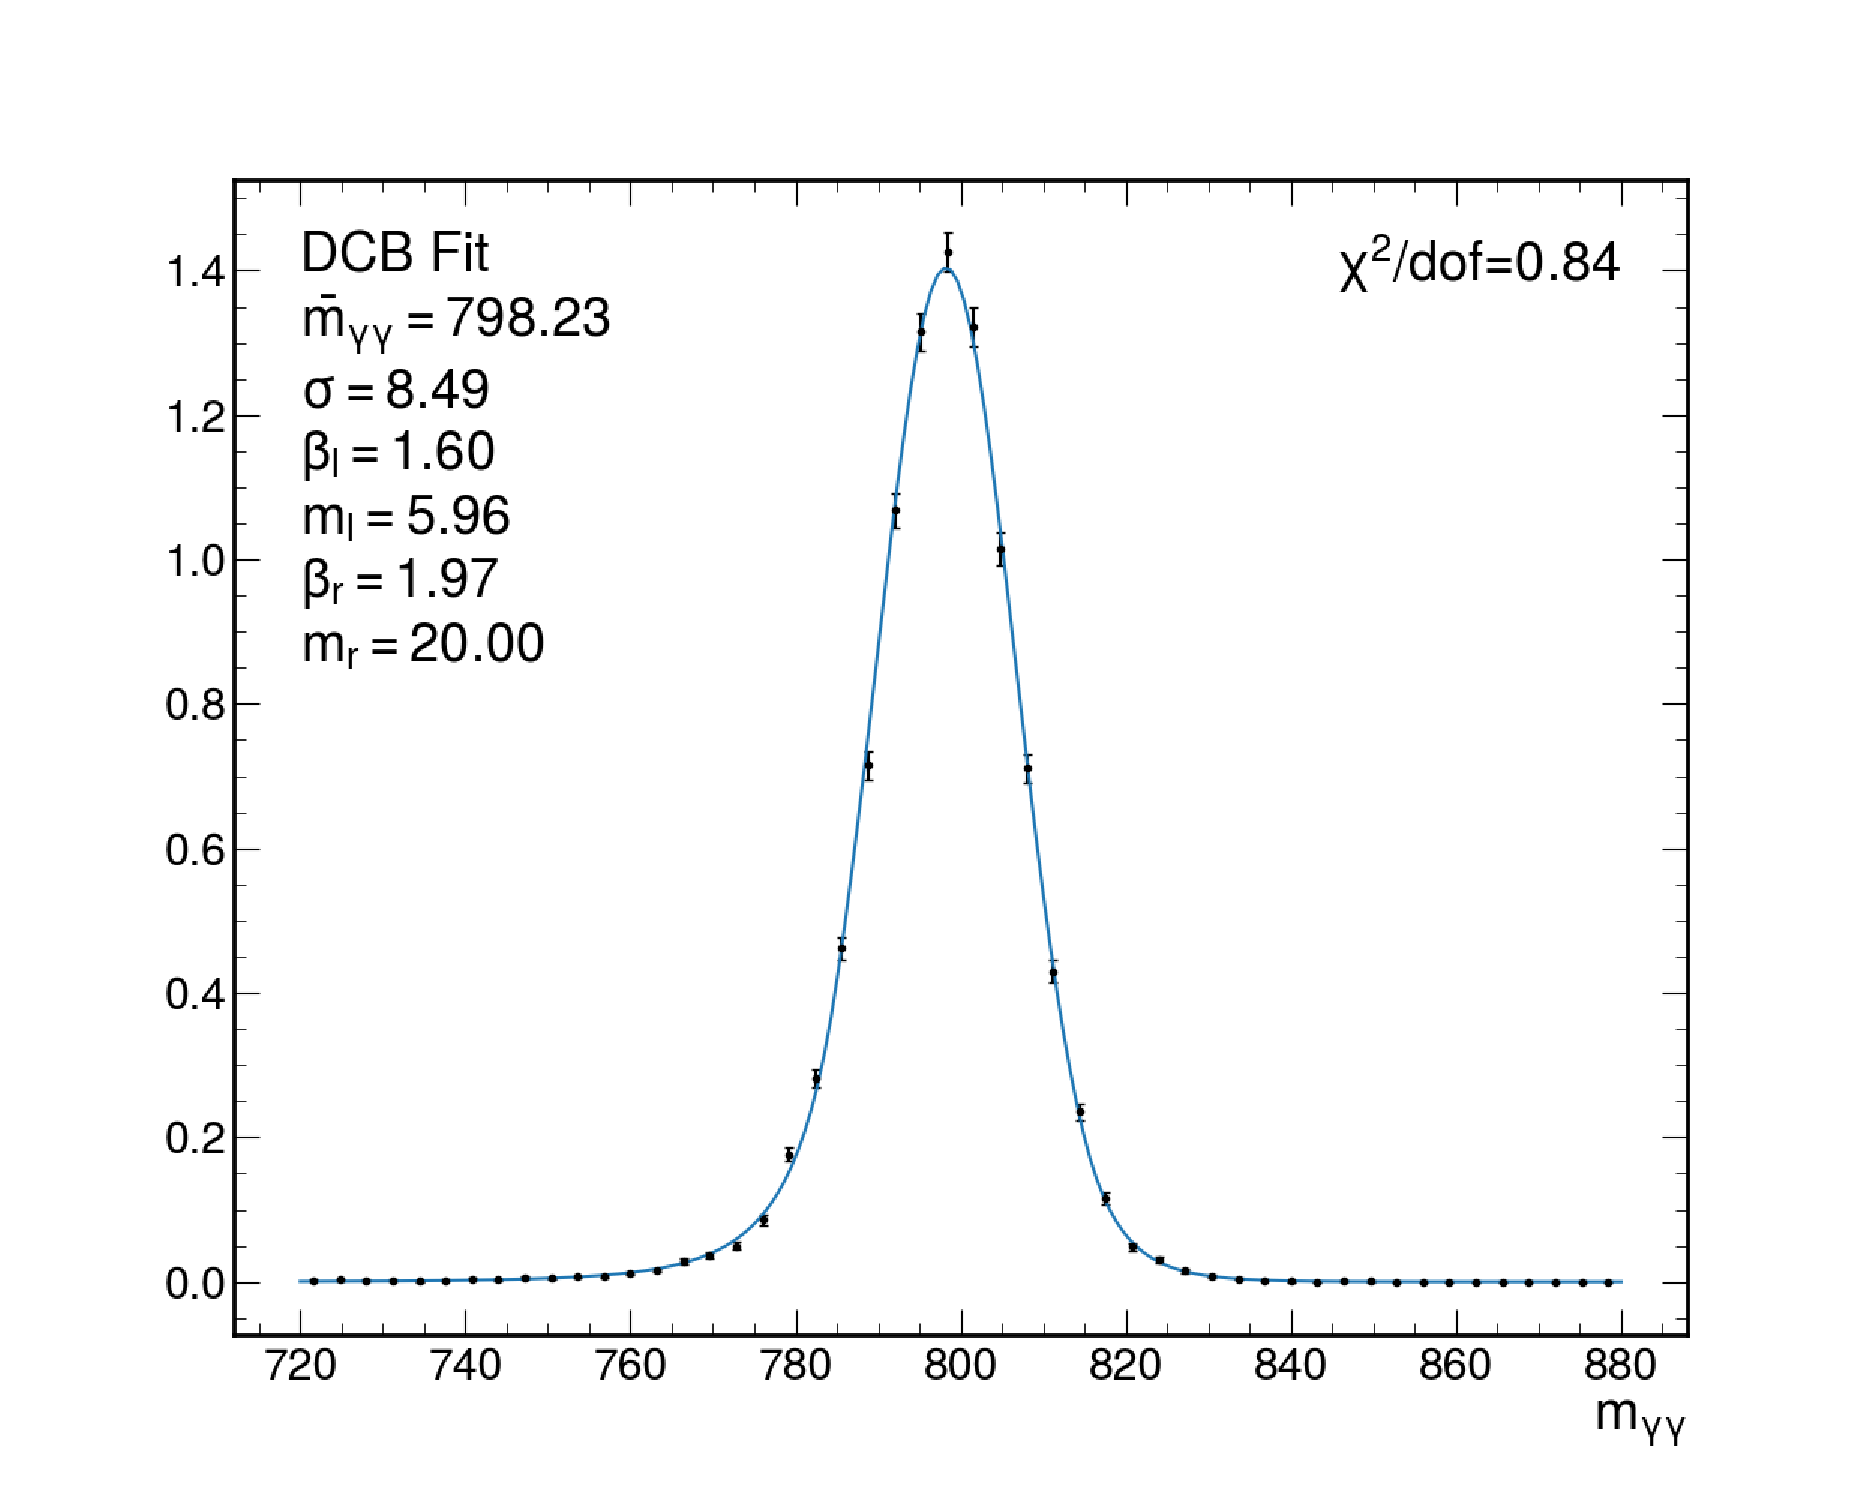
\includegraphics[width=0.49\textwidth]{Figures/Dihiggs/signal/high_mass_mx_1000_my_800.pdf}
  \caption[DCB Signal Fits in \XYH Searches]{DCB fits in category 0 in 2018 for the \XYttHgg search (top) and \XYggHtt search (bottom). The mass points are $(\mX,\mY)=(600,90)$ (top-left), $(300,70)$ (top-right), $(600,90)$ (bottom-left), and $(1000,800)$\GeV (bottom-right).}\label{fig:dcb_fits}
\end{figure}

To study the impact of a nuisance parameter on the modelling of the single and di-Higgs processes, simulated datasets are created when changing the nuisance parameter to $\nu=-1$ or $\nu=1$, which are referred to as down and up variations respectively. These datasets are created either by reweighting the nominal dataset ($\nu=0$), or by rerunning the simulation with $\nu=-1$ or $\nu=1$, where the approach taken depends on the nuisance parameter. Typically, nuisance parameters related to ID scale factors take the former approach, and nuisance parameters related to energy scale and resolution corrections take the latter approach. The $\kappa$ factors that describe the impact of a nuisance parameter are derived by taking the ratio of the expected number of events in the up and down variations to the expected number of events in the nominal variation. 

The derivation of the $\alpha$ parameters is more involved. Firstly, only the effect of a nuisance parameter on $\hat{m}_{\gamma\gamma}$ and $\sigma$ is studied. The impact on all other shape parameters of the DCB are assumed to be negligible. Instead of refitting the DCB to the up and down variations, proxy variables are used to describe the changes in $\hat{m}_{\gamma\gamma}$ and $\sigma$. For $\hat{m}_{\gamma\gamma}$, this is simply the mean of the \mgg distribution, and for $\sigma$, it is the smallest \mgg interval that contains 68\% of the distribution, which for a Gaussian distribution, would be equivalent to the standard deviation. Then the ratio of the proxy variable in the up and down variations to the proxy variable in the nominal variation is taken, and the average of those ratios is taken as the $\alpha$ parameter. In the \XTwoHH search in category 0, the average value of $\alpha$ for the photon energy scale calibration is 0.005 and 0.014 for $\hat{m}_{\gamma\gamma}$ and $\sigma$ respectively, and in the high-mass \XYggHtt search, the equivalent numbers are 0.01 and 0.04. 

\subsubsection{Intermediate Mass Points}\label{sec:modelling_intermediate_mass_points}
For the single Higgs processes, the modelling at the intermediate mass points follows the same methods described above since an analysis at an intermediate mass point just corresponds to different selection on the pNN score. 

For the di-Higgs processes at the intermediate mass points, $\epsilon$ and $\vec{\Psi}$ are determined from the values found at the closest nominal mass point, or by interpolating the values found with neighbouring nominal mass points, depending on the parameter. The choice of which approach to take is motivated by the level of dependence of the parameter on \mX and \mY. \Cref{fig:graviton_sigeff_change} shows $\epsilon$ at the nominal mass points as a function of \mX in the \XTwoHH search when selecting $\tilde{f}(\vec{x};\mX)$ in ranges of 0.98--0.99 or 0.99--1.0. These plots show that the $\epsilon$ can change significantly between mass points, motivating the use of interpolation methods. 

\begin{figure}
  \centering
  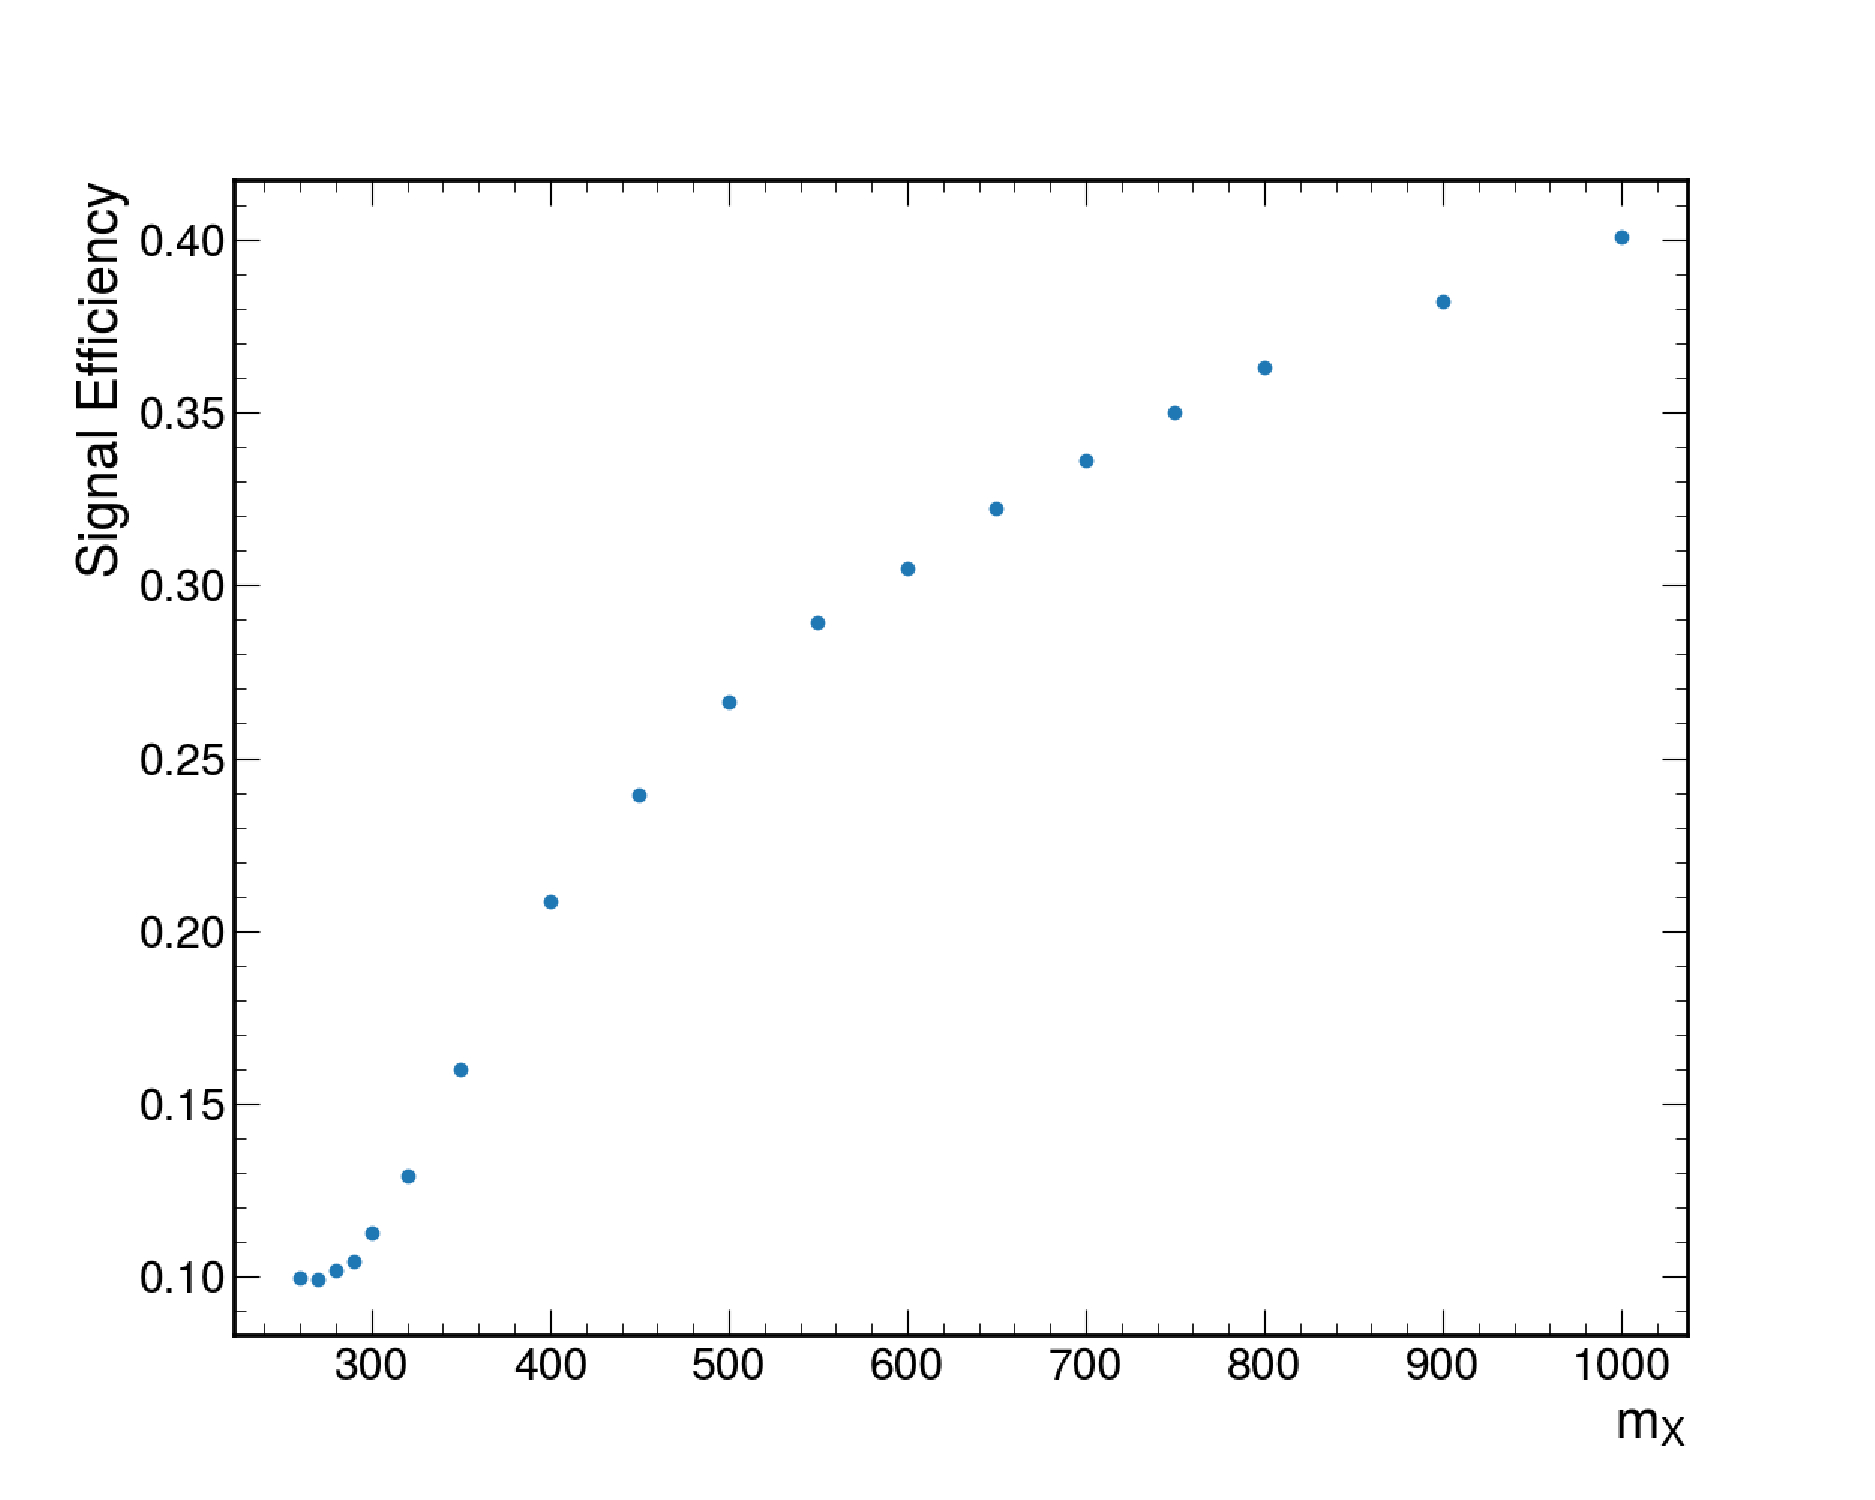
\includegraphics[width=0.49\textwidth]{Figures/Dihiggs/signal/shape_change/graviton_sigeff.pdf}
  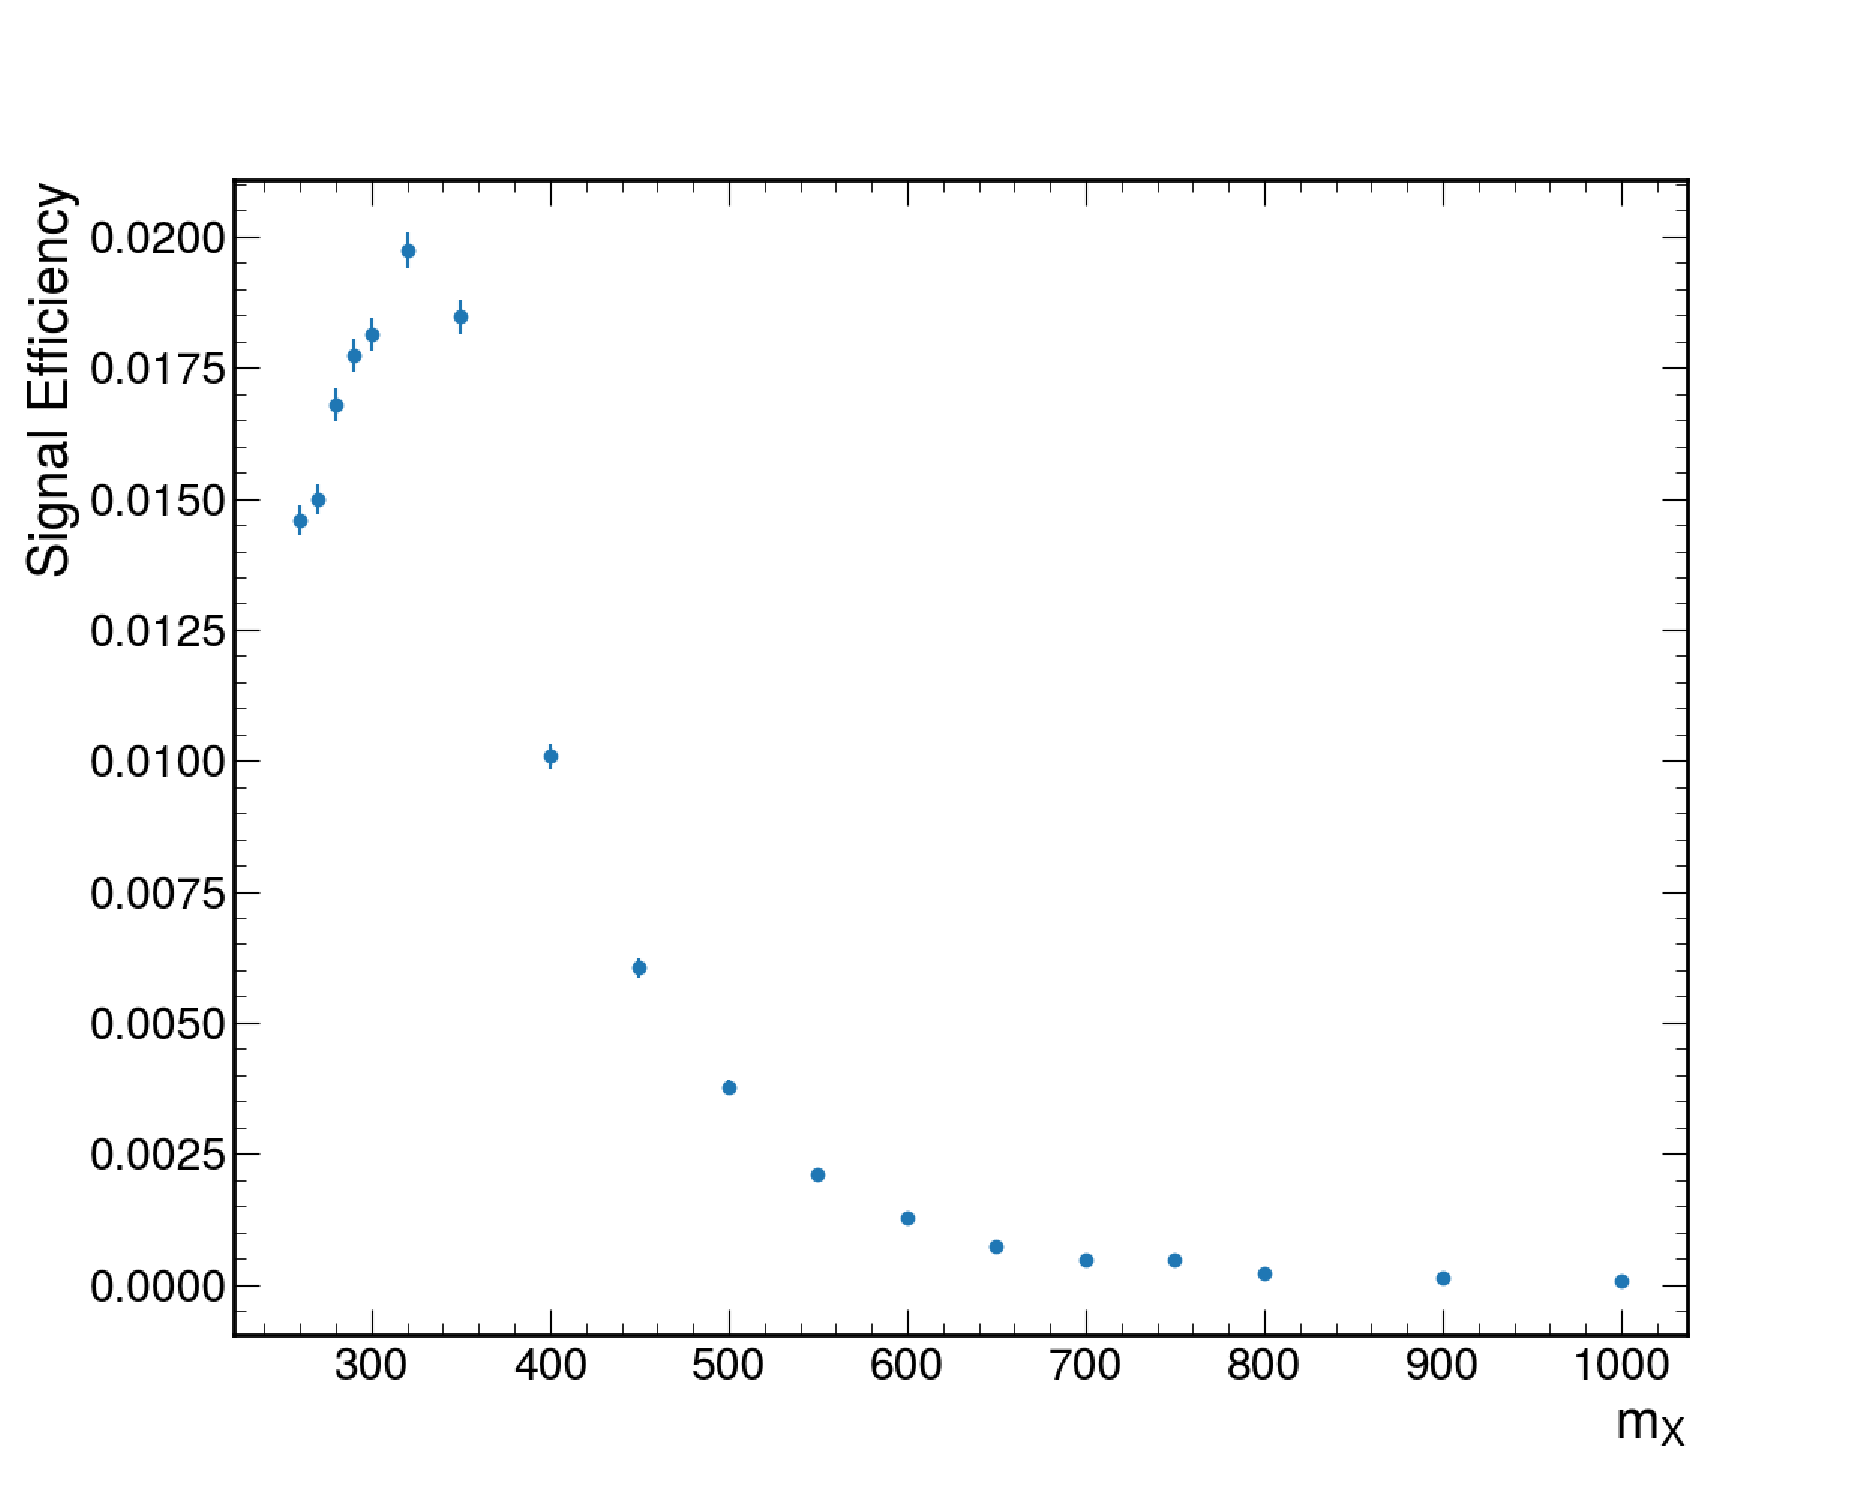
\includegraphics[width=0.49\textwidth]{Figures/Dihiggs/signal/shape_change/graviton_sigeff_less.pdf}
  \caption[Signal Efficiencies as a Function of \mX in \XTwoHH Search]{Signal efficiency as a function of \mX for the \XTwoHH averaged over years. On the left, a requirement of $\tilde{f}(\vec{x};\mX) > 0.99$ is placed, and on the right, a requirement of $0.98 < \tilde{f}(\vec{x};\mX) < 0.99$. These requirements illustrate the trends seen in the purest category and a less-pure category respectively.}\label{fig:graviton_sigeff_change}
\end{figure}

To determine $\epsilon$ at an intermediate mass point, $\mX^{\text{int}}$, in the \XHH searches, for a category defined by $b_1 < \tilde{f}(\vec{x};\mX^{\text{int}}) < b_2$, linear and cubic splines are created from the $\epsilon$ values derived using the nominal MC samples with selections: $b_1 < \tilde{f}(\vec{x};\mX) < b_2$. Examples of this for category 0 and category 1 for $\mX=375$ and 433\GeV in the \XTwoHH search are shown in \cref{fig:graviton_example_splines1}. To study the robustness of the splines, they are recreated when removing the nominal mass point closest to $\mX^{\text{int}}$, and the difference between the splines at $\mX^{\text{int}}$ is calculated. Then, the value for $\epsilon$ at $\mX^{\text{int}}$ is given by the linear or cubic spline derived using all mass nominal points, depending on which type minimizes this difference. A systematic uncertainty is then assigned to $\epsilon$ using the difference found for the chosen spline.

\begin{figure}
  \centering
  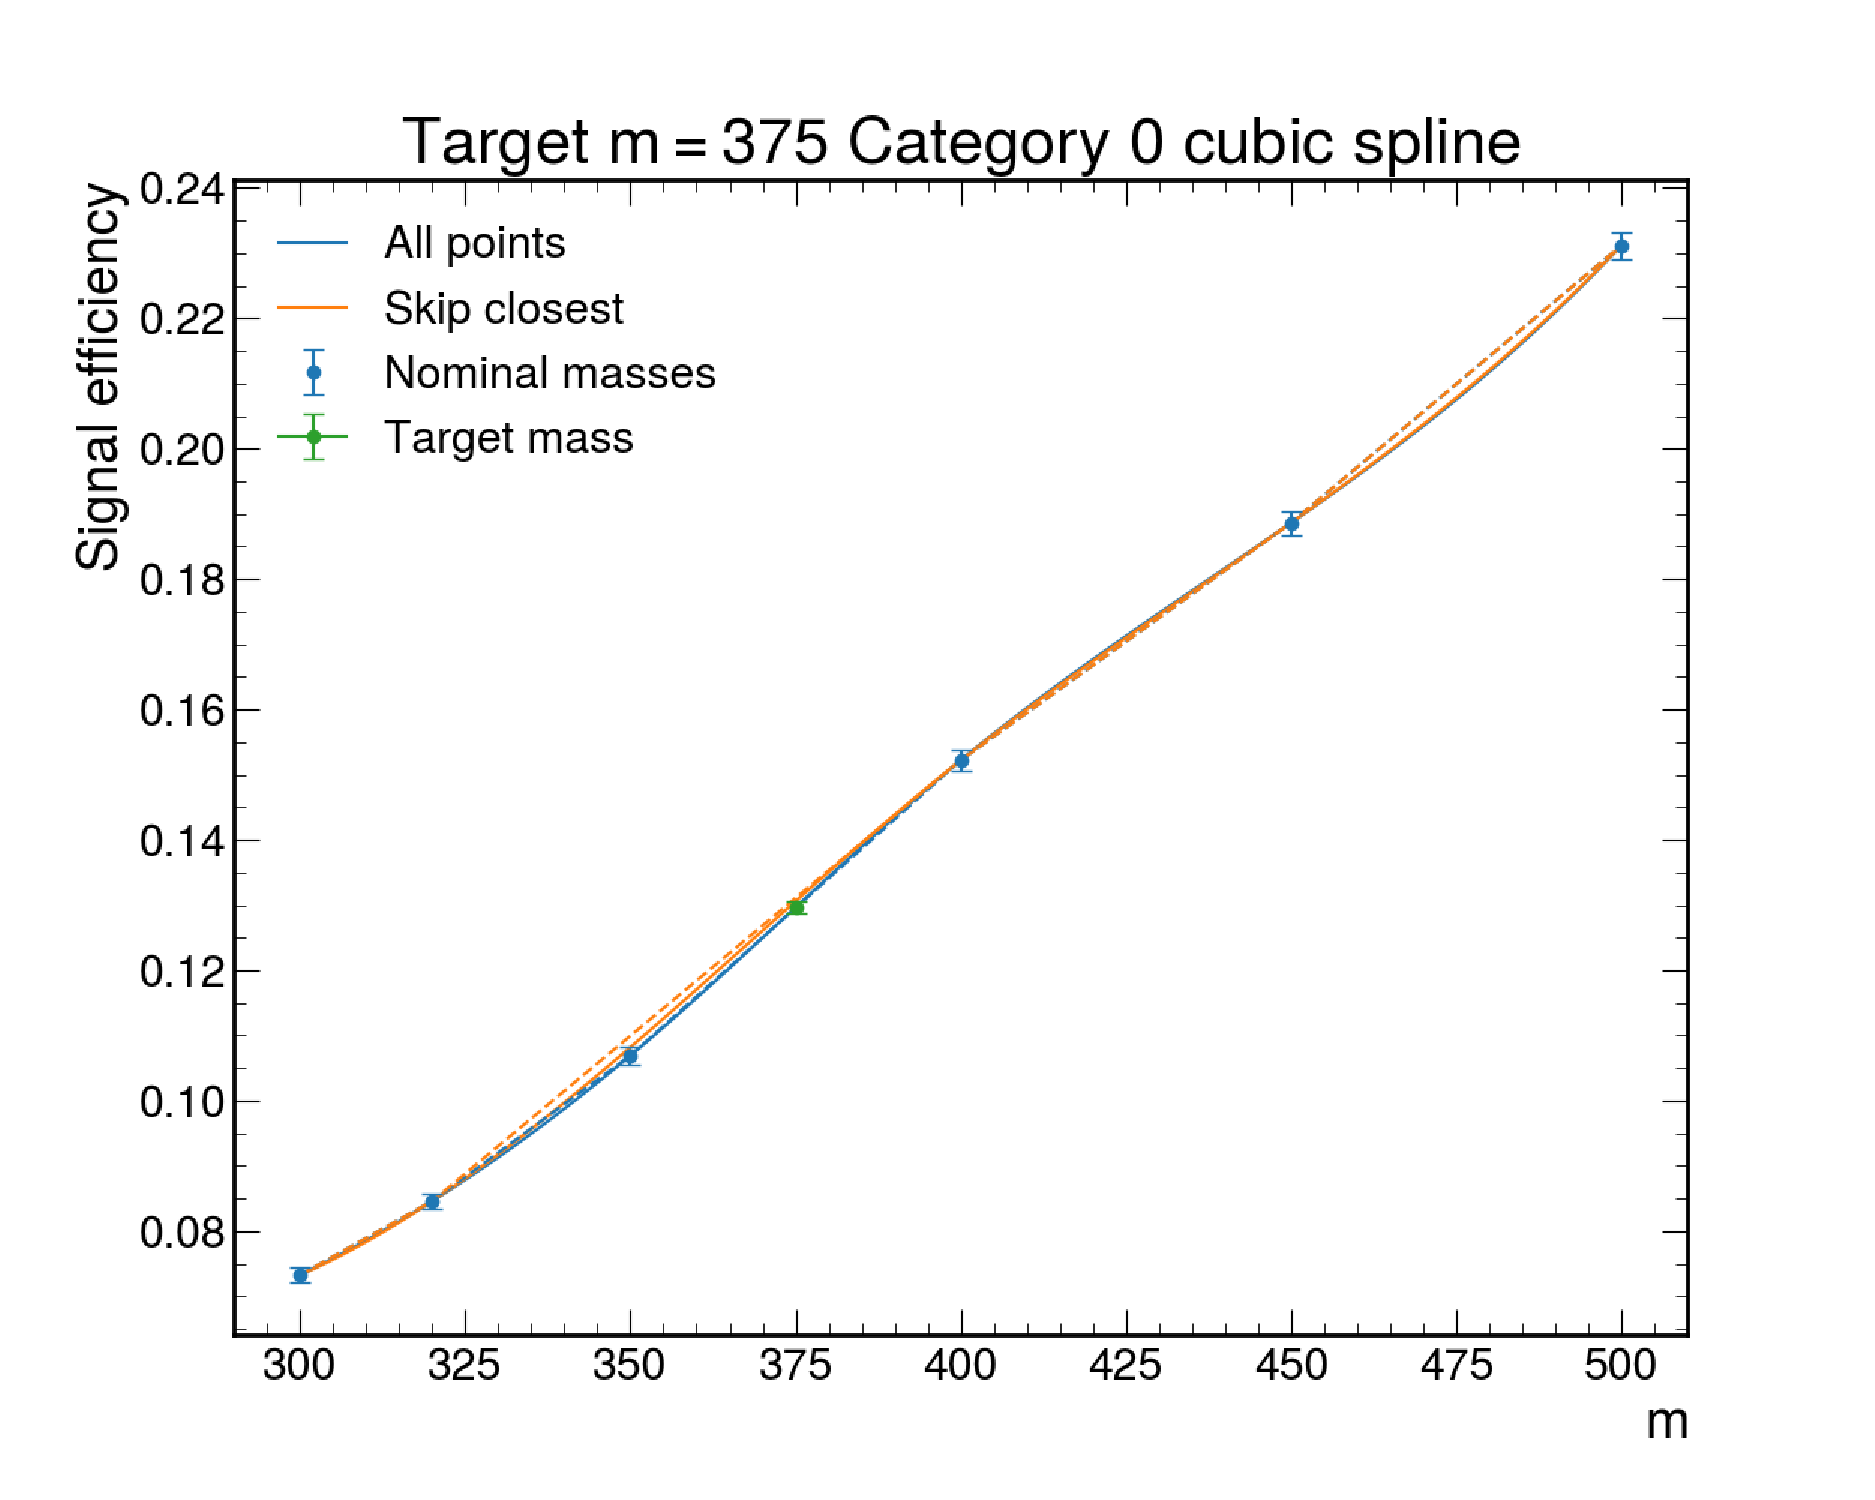
\includegraphics[width=0.7\textwidth]{Figures/Dihiggs/signal/sigeff_interpolation/graviton_375_2018_cat0_interpolation.pdf} \\
  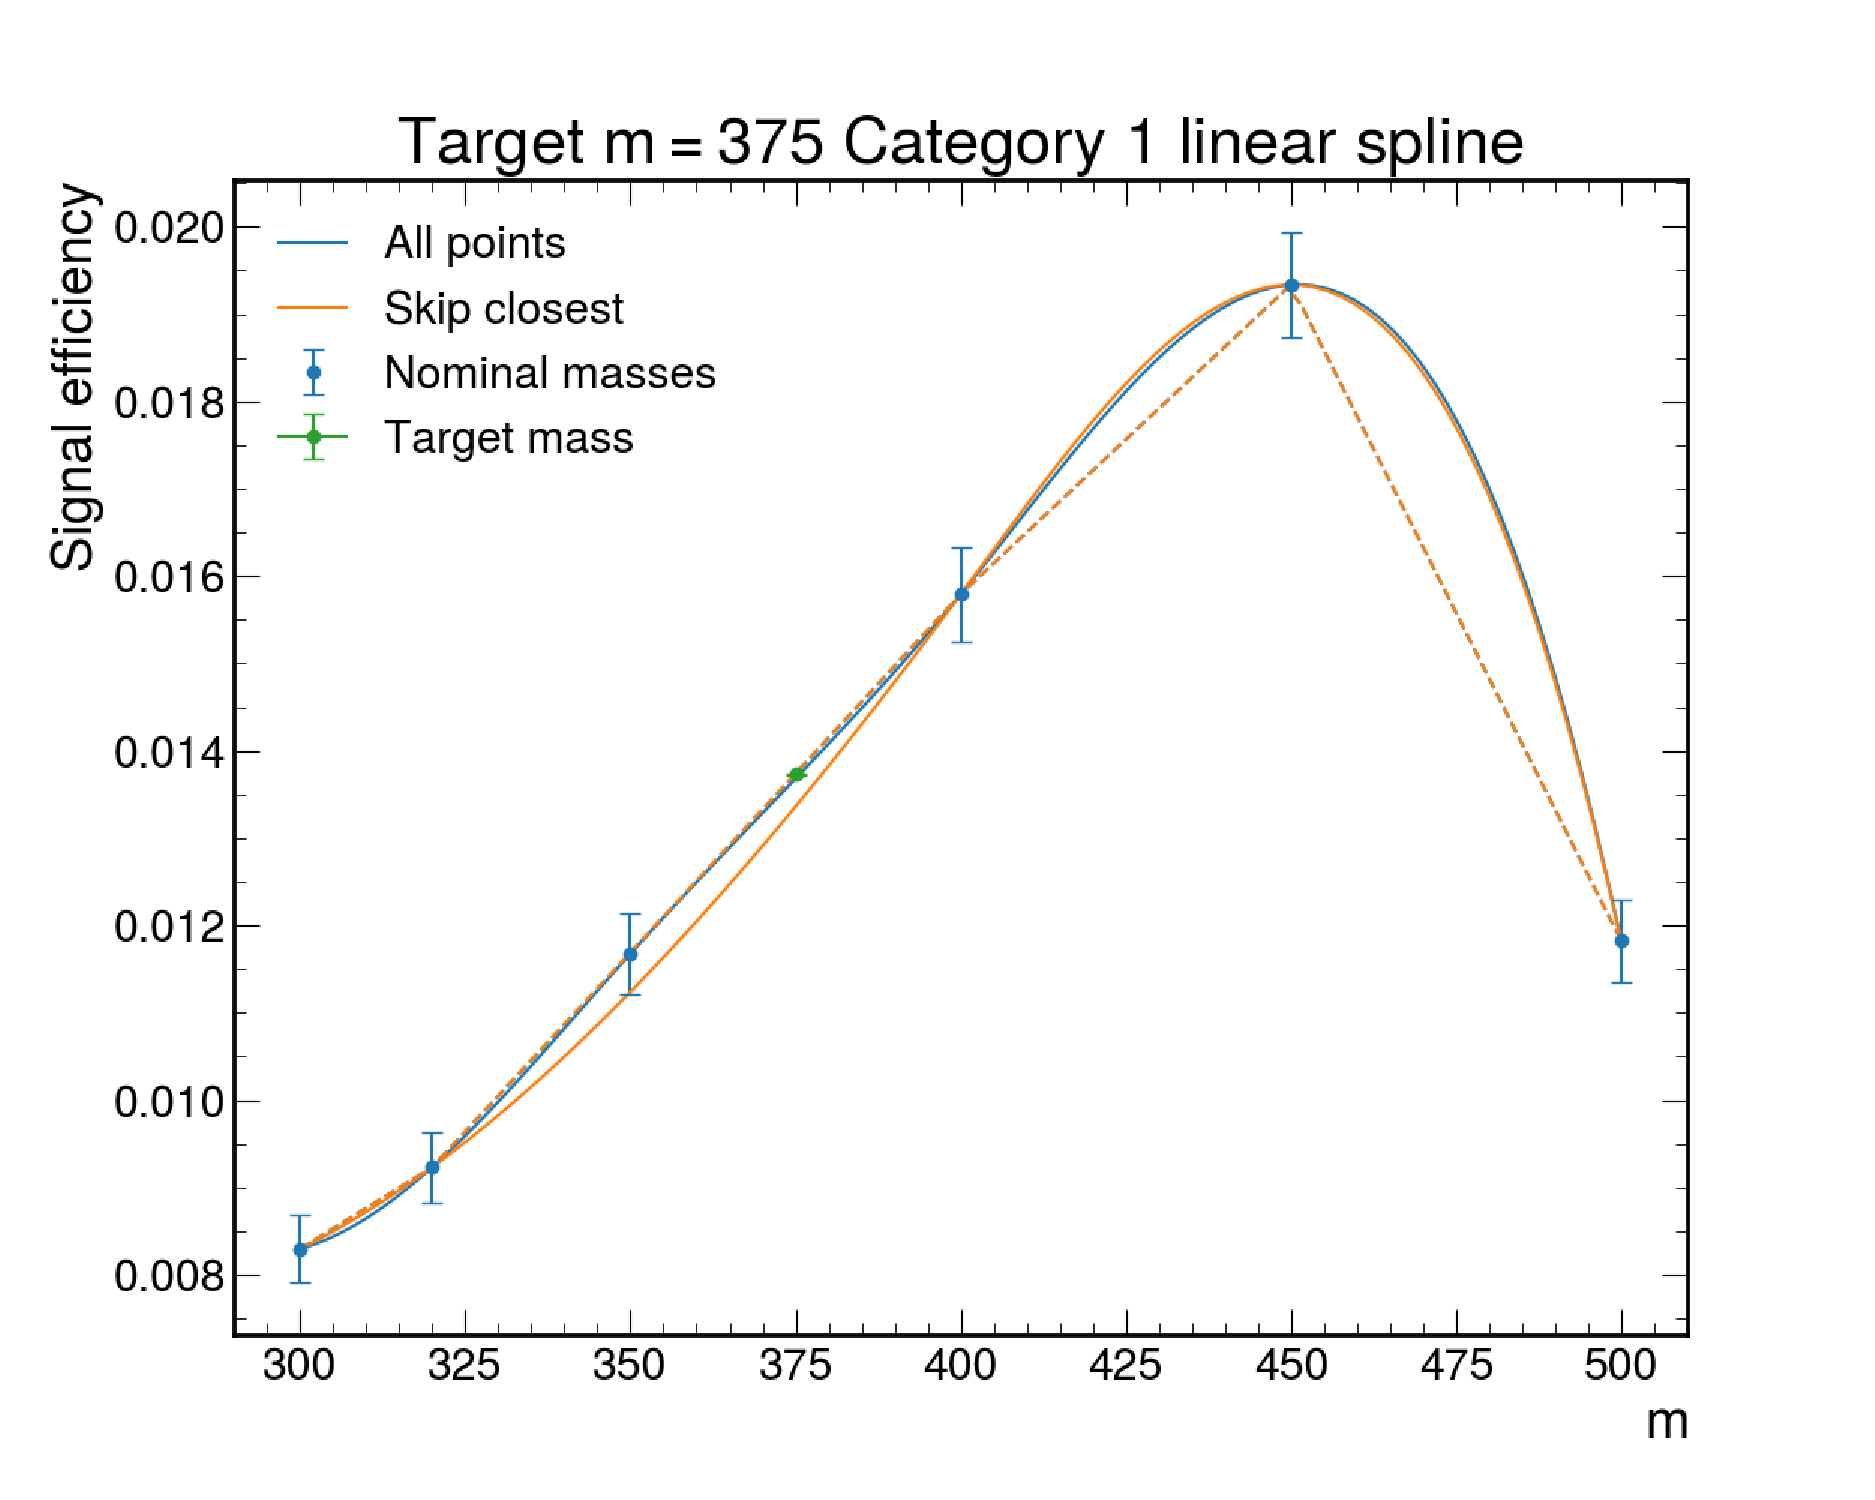
\includegraphics[width=0.7\textwidth]{Figures/Dihiggs/signal/sigeff_interpolation/graviton_375_2018_cat1_interpolation.pdf}
  \caption[Signal Efficiency Splines for $\mX=375$\GeV in the \XTwoHH Search]{Splines used to estimate the signal efficiency for $\mX=375$ in the \XTwoHH search in 2018 for category 0 (top) and category 1 (bottom). In the plots, $m$ refers to $\mX$. The solid and dashed lines are cubic and linear splines respectively and the spline type chosen to calculate the signal efficiency is specified in the plot title. The uncertainty in the interpolated signal efficiency (at $m_X=375$) is shown by the green error bar and is taken from the difference between the spline found when using all nominal mass points and the spline found when skipping the closest mass point.}\label{fig:graviton_example_splines1}
\end{figure}

\begin{figure}
  \centering
  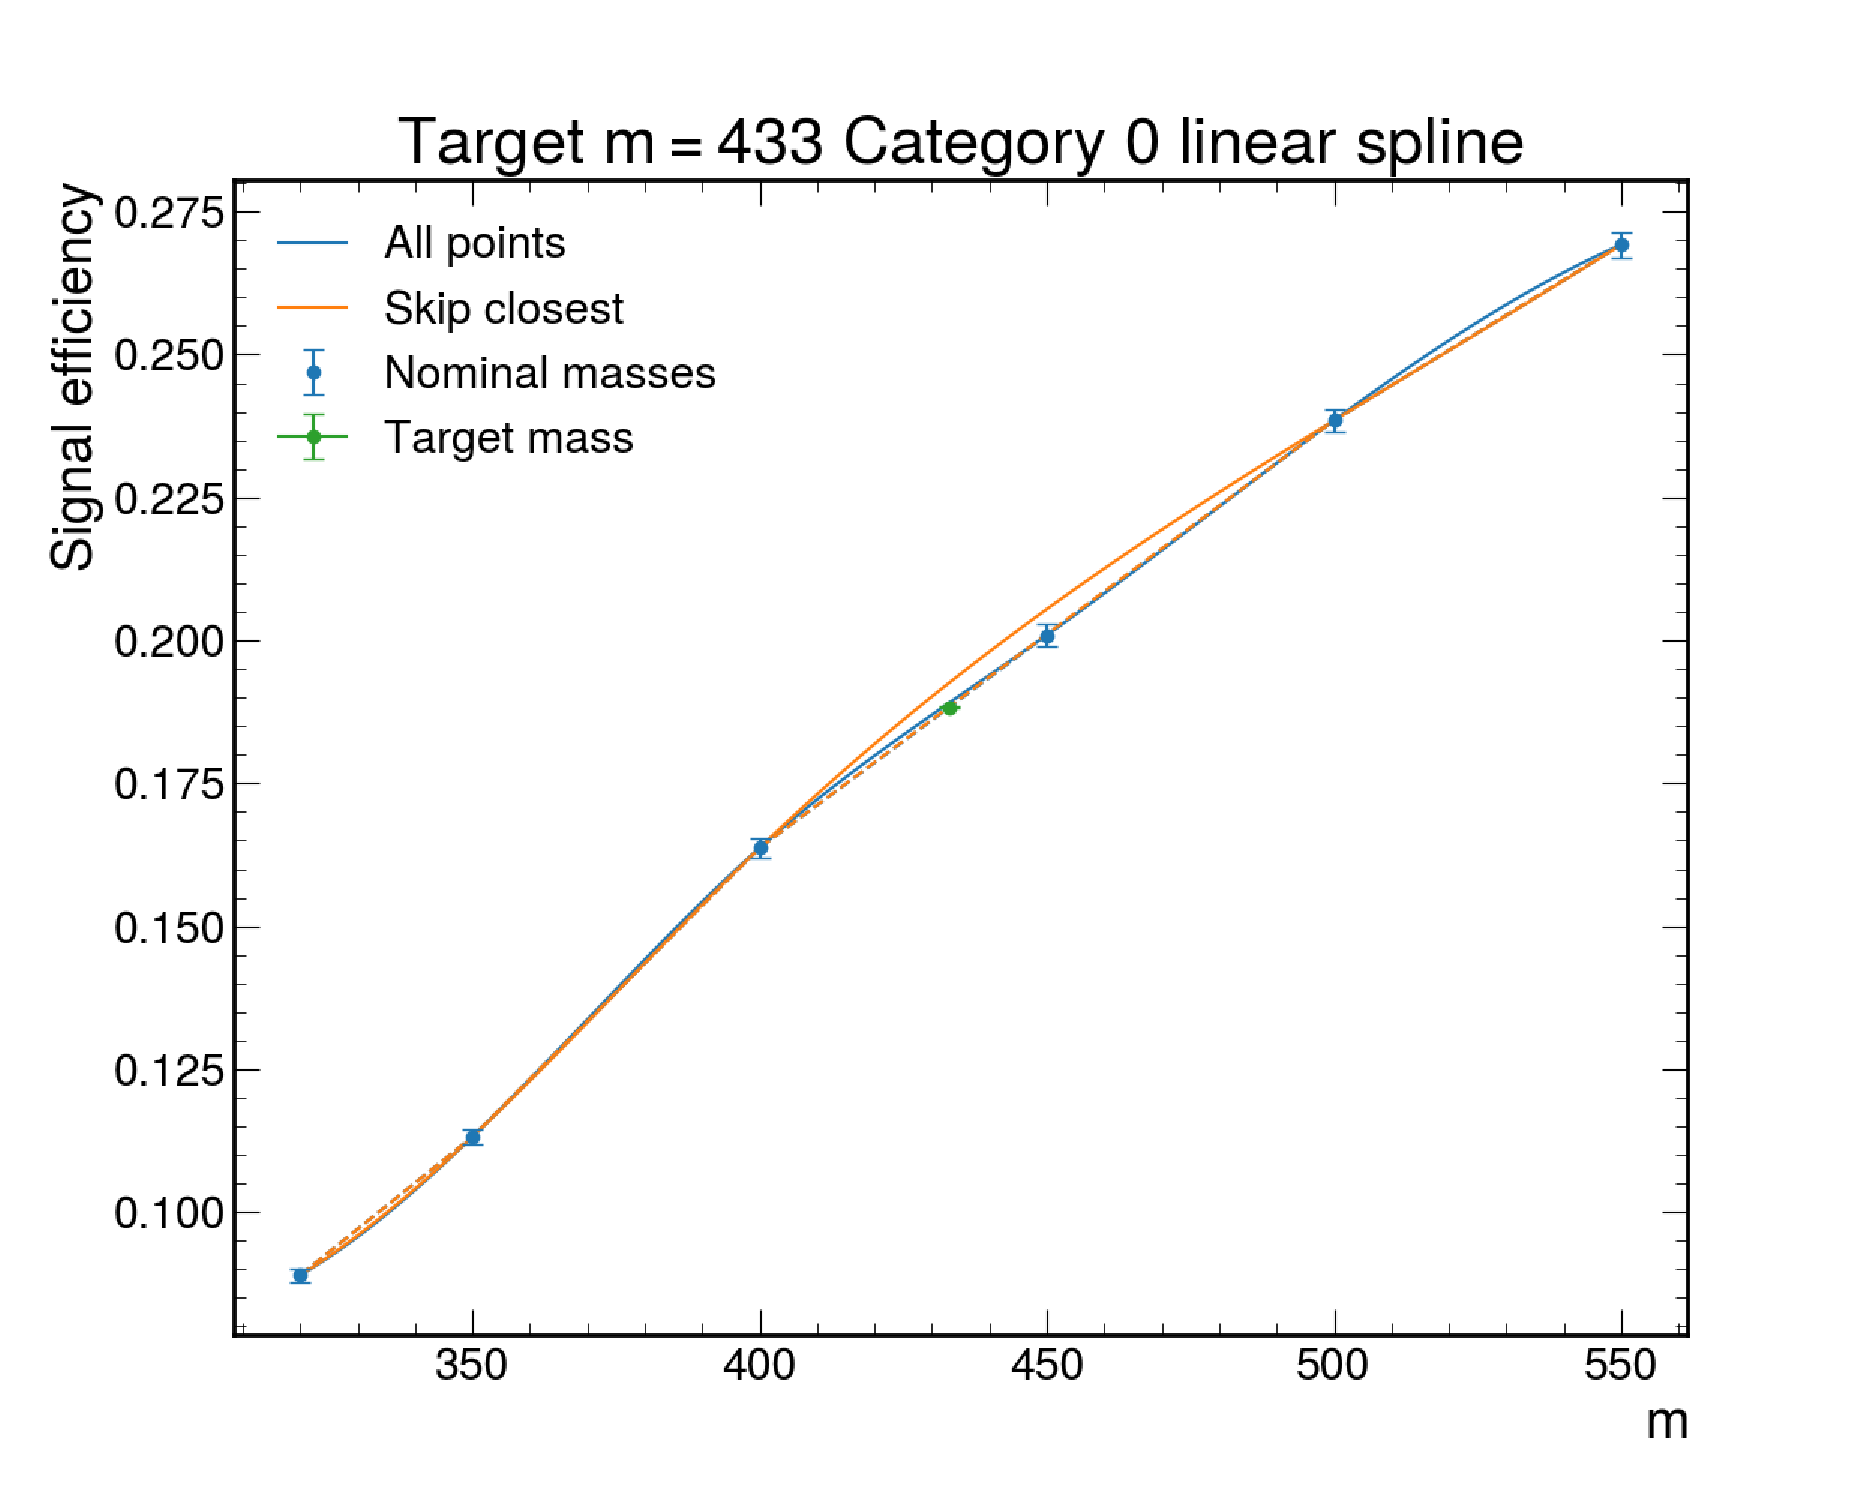
\includegraphics[width=0.7\textwidth]{Figures/Dihiggs/signal/sigeff_interpolation/graviton_433_2018_cat0_interpolation.pdf} \\
  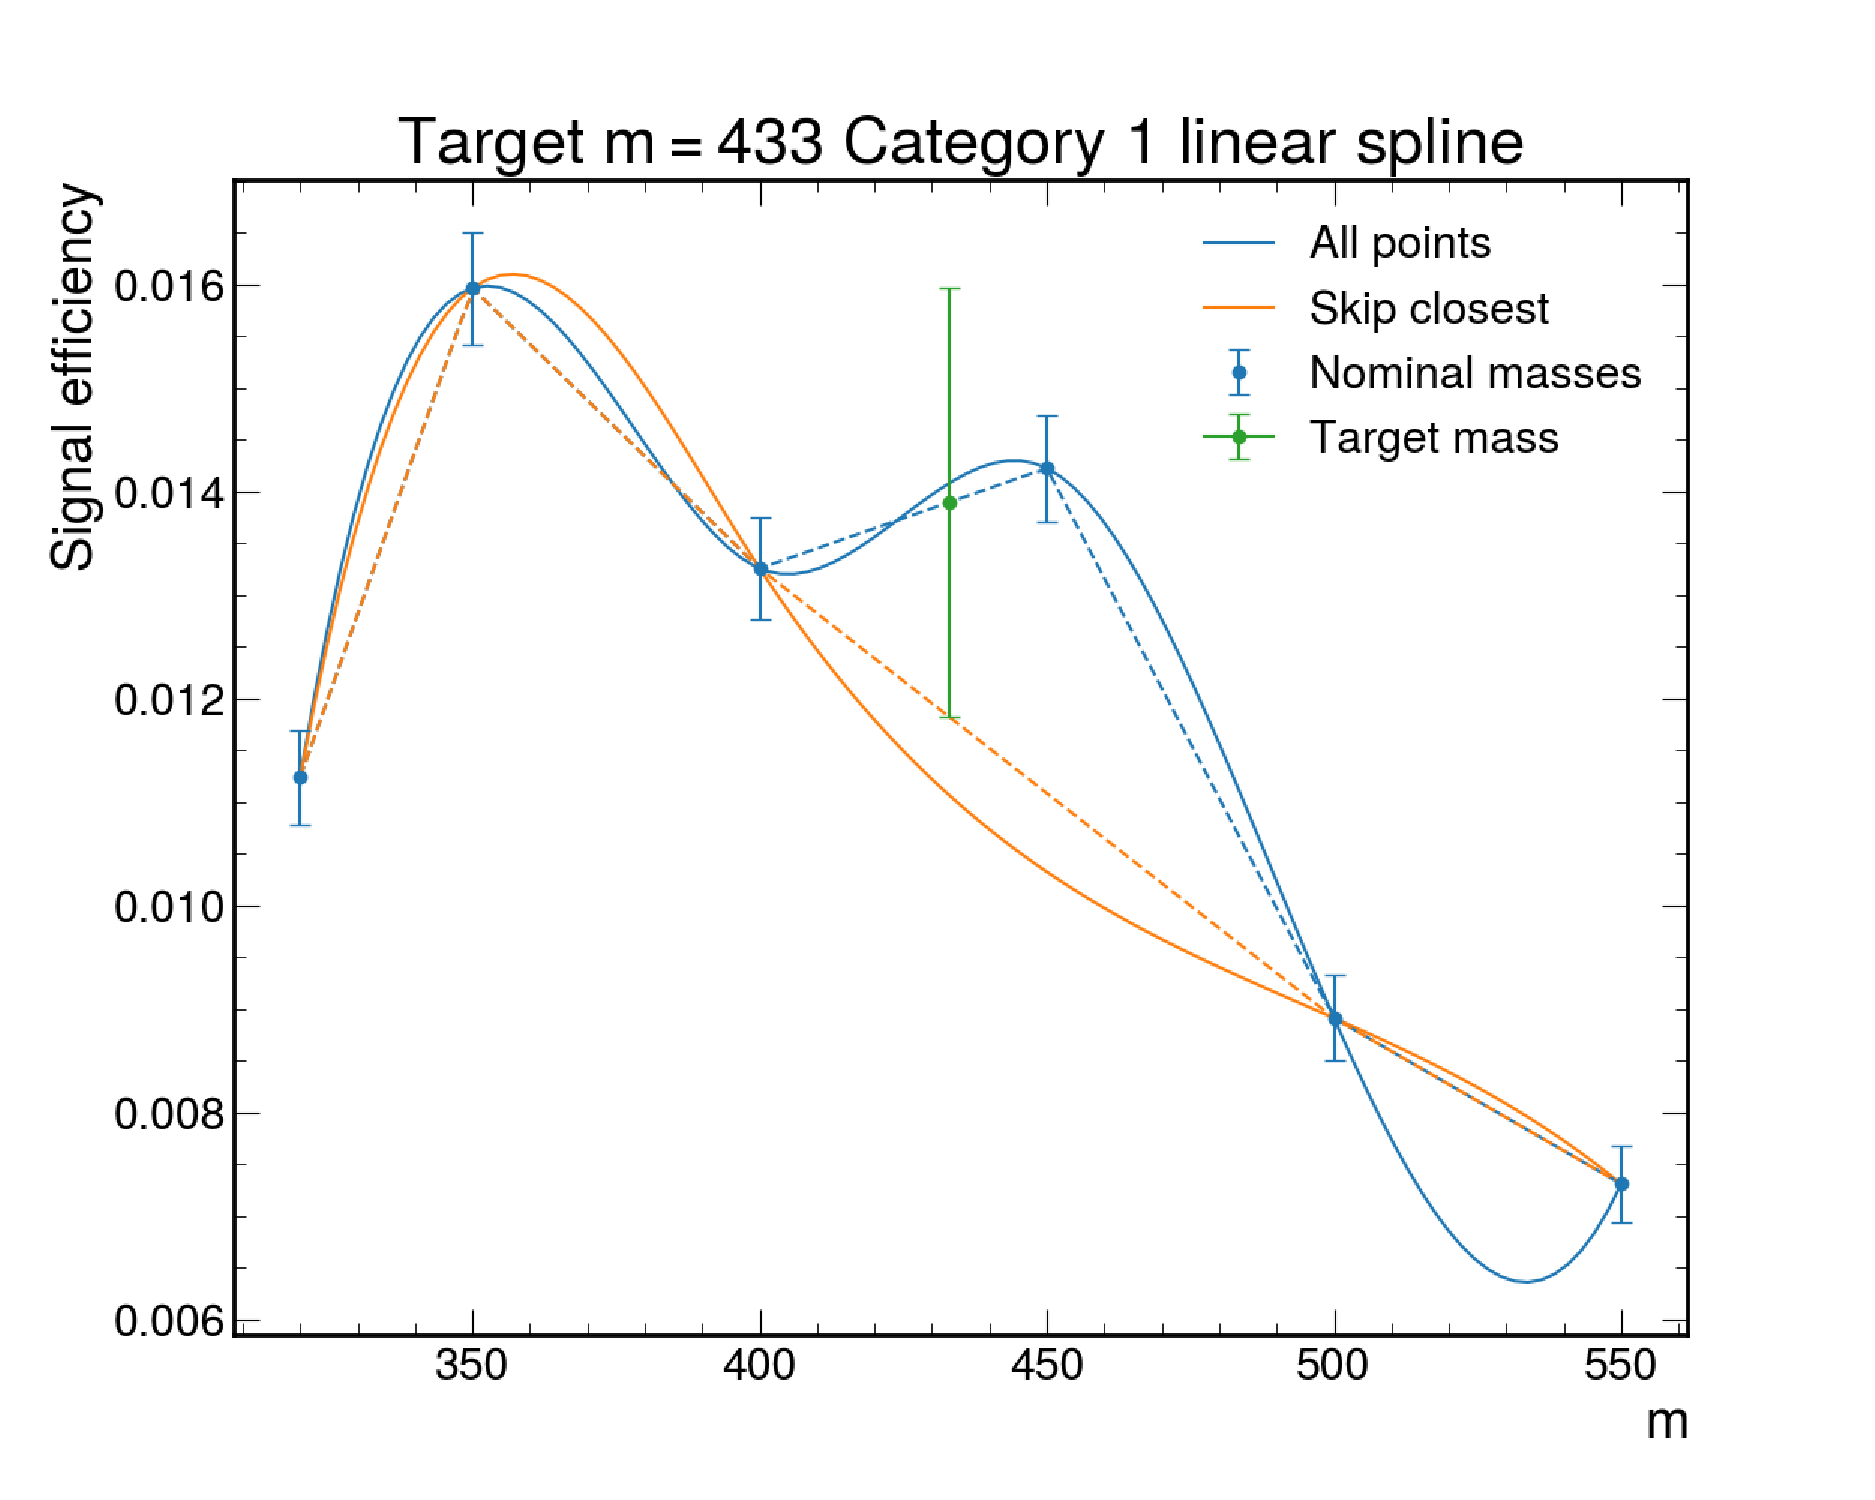
\includegraphics[width=0.7\textwidth]{Figures/Dihiggs/signal/sigeff_interpolation/graviton_433_2018_cat1_interpolation.pdf}
  \caption[Signal Efficiency Splines for $\mX=433$\GeV in the \XTwoHH Search]{Splines used to estimate the signal efficiency for $\mX=433$ in the \XTwoHH search in 2018 for category 0 (top) and category 1 (bottom). In the plots, $m$ refers to $\mX$. The solid and dashed lines are cubic and linear splines respectively and the spline type chosen to calculate the signal efficiency is specified in the plot title. The uncertainty in the interpolated signal efficiency (at $m_X=$) is shown by the green error bar and is taken from the difference between the spline found when using all nominal mass points and the spline found when skipping the closest mass point.}\label{fig:graviton_example_splines2}
\end{figure}

\Cref{fig:graviton_shape_change} shows how the shape parameters of the DCB change at the nominal mass points as a function of \mX in the \XTwoHH search when selecting $\tilde{f}(\vec{x};\mX)$ in the range 0.99--1.0. In these plots, the dependence on $\hat{m}_{\gamma\gamma}$ is shown via $\Delta\mgg = \hat{m}_{\gamma\gamma}-125\GeV$. The $\Delta\mgg$, $\sigma$, and $\beta_l$ shape parameters are seen to change significantly enough between mass points to justify the use of interpolation methods. The approach is the same as for $\epsilon$, except that only linear splines are used, and no systematic uncertainty is assigned to the interpolated shape parameters. The values of $\beta_r$, $m_l$, and $m_r$, show smaller dependence on \mX, and are therefore fixed to the values found at the closest nominal mass point. 

\begin{figure}
  \centering
  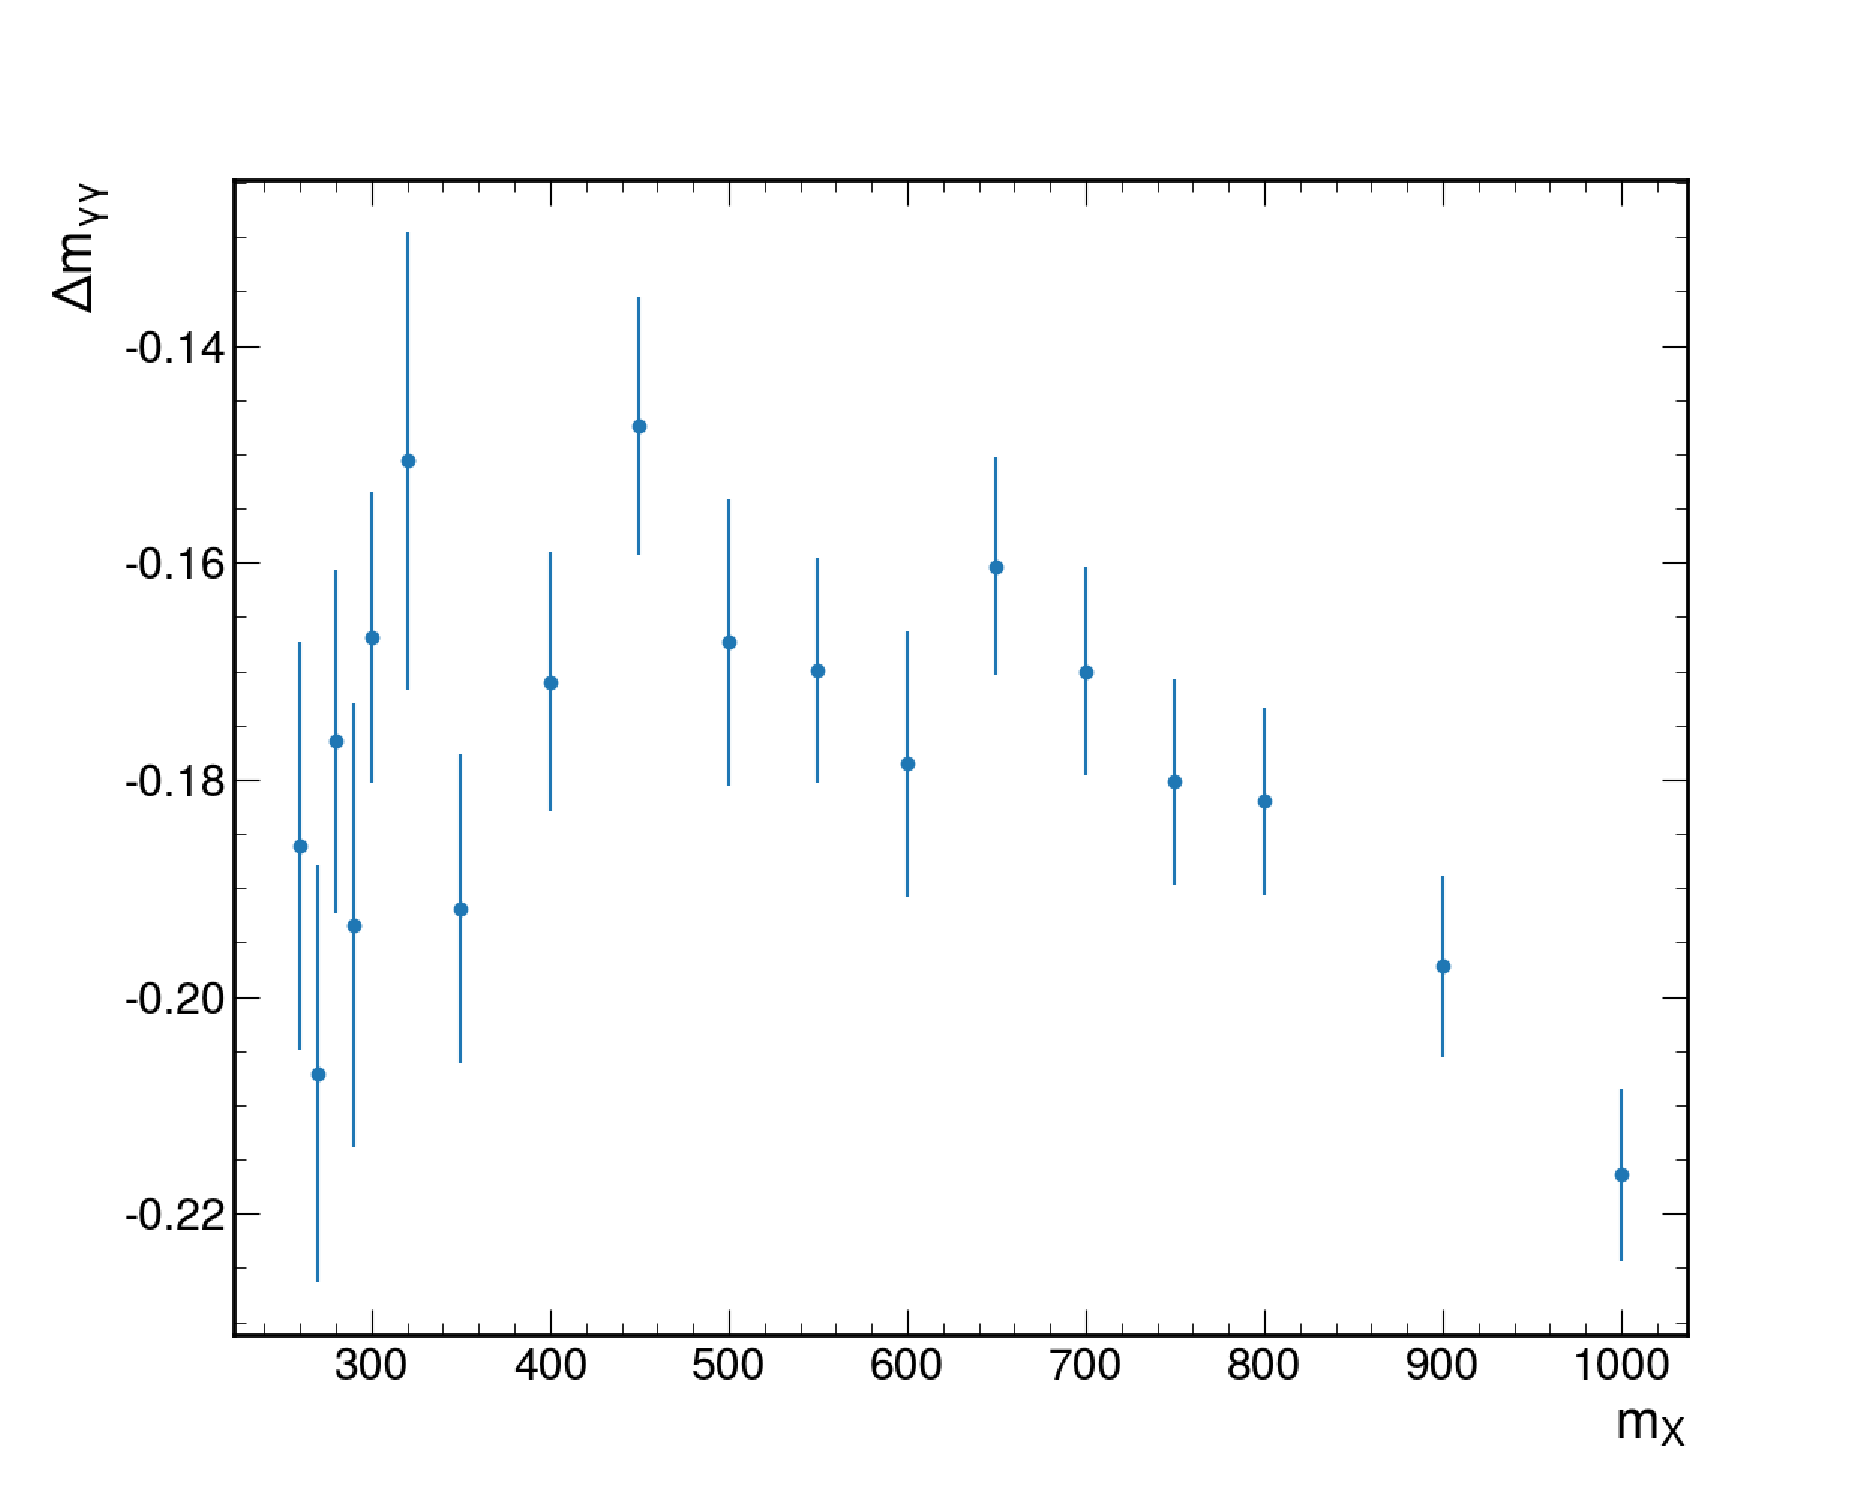
\includegraphics[width=0.49\textwidth]{Figures/Dihiggs/signal/shape_change/graviton_dm.pdf}
  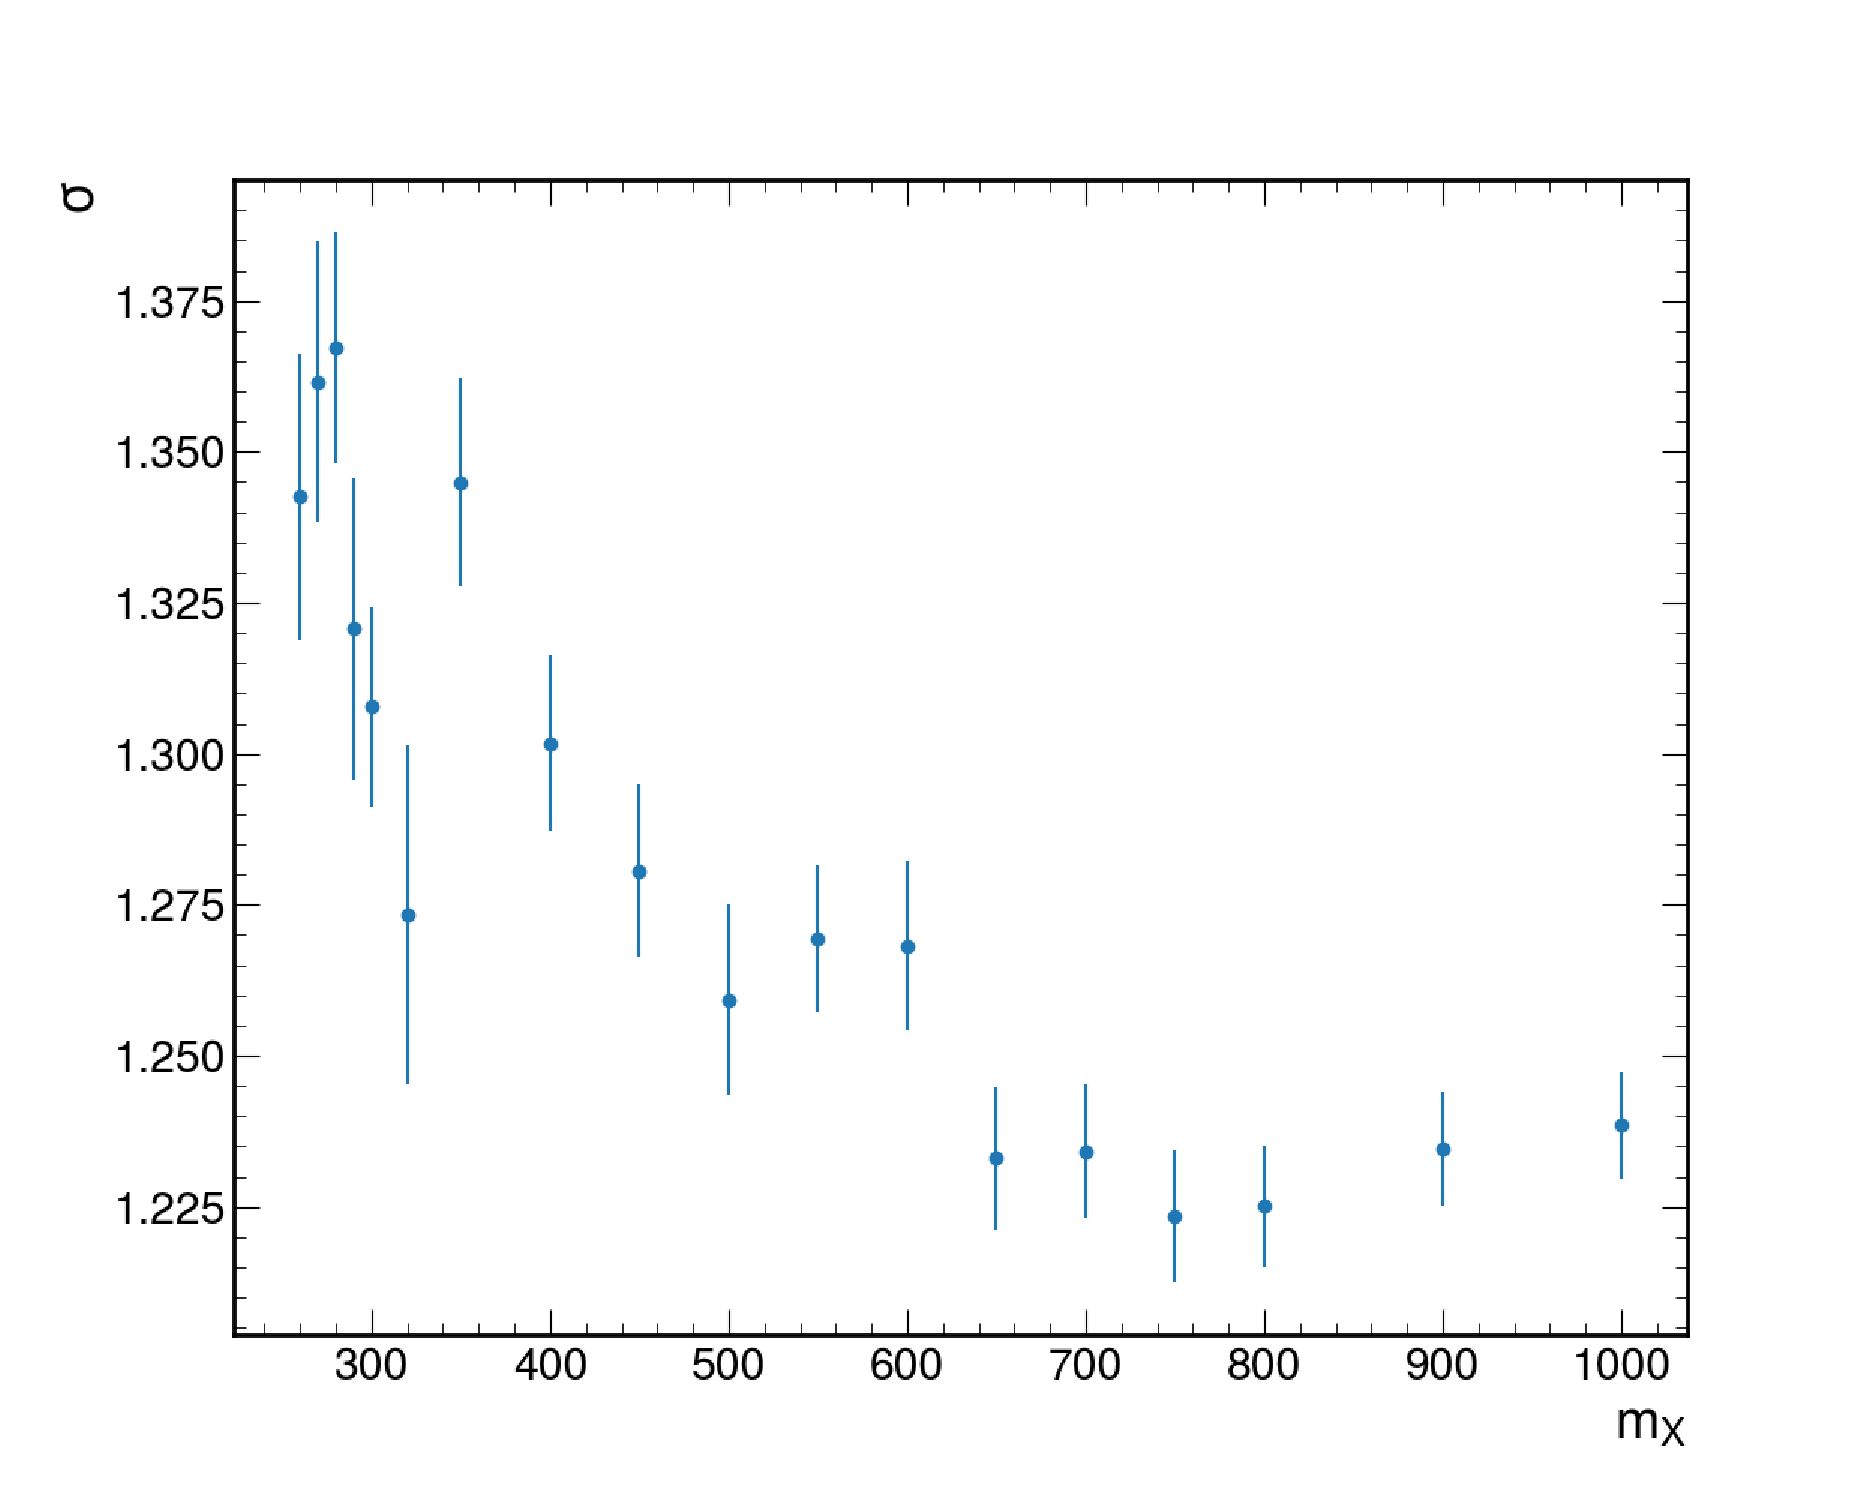
\includegraphics[width=0.49\textwidth]{Figures/Dihiggs/signal/shape_change/graviton_sigma.pdf} \\
  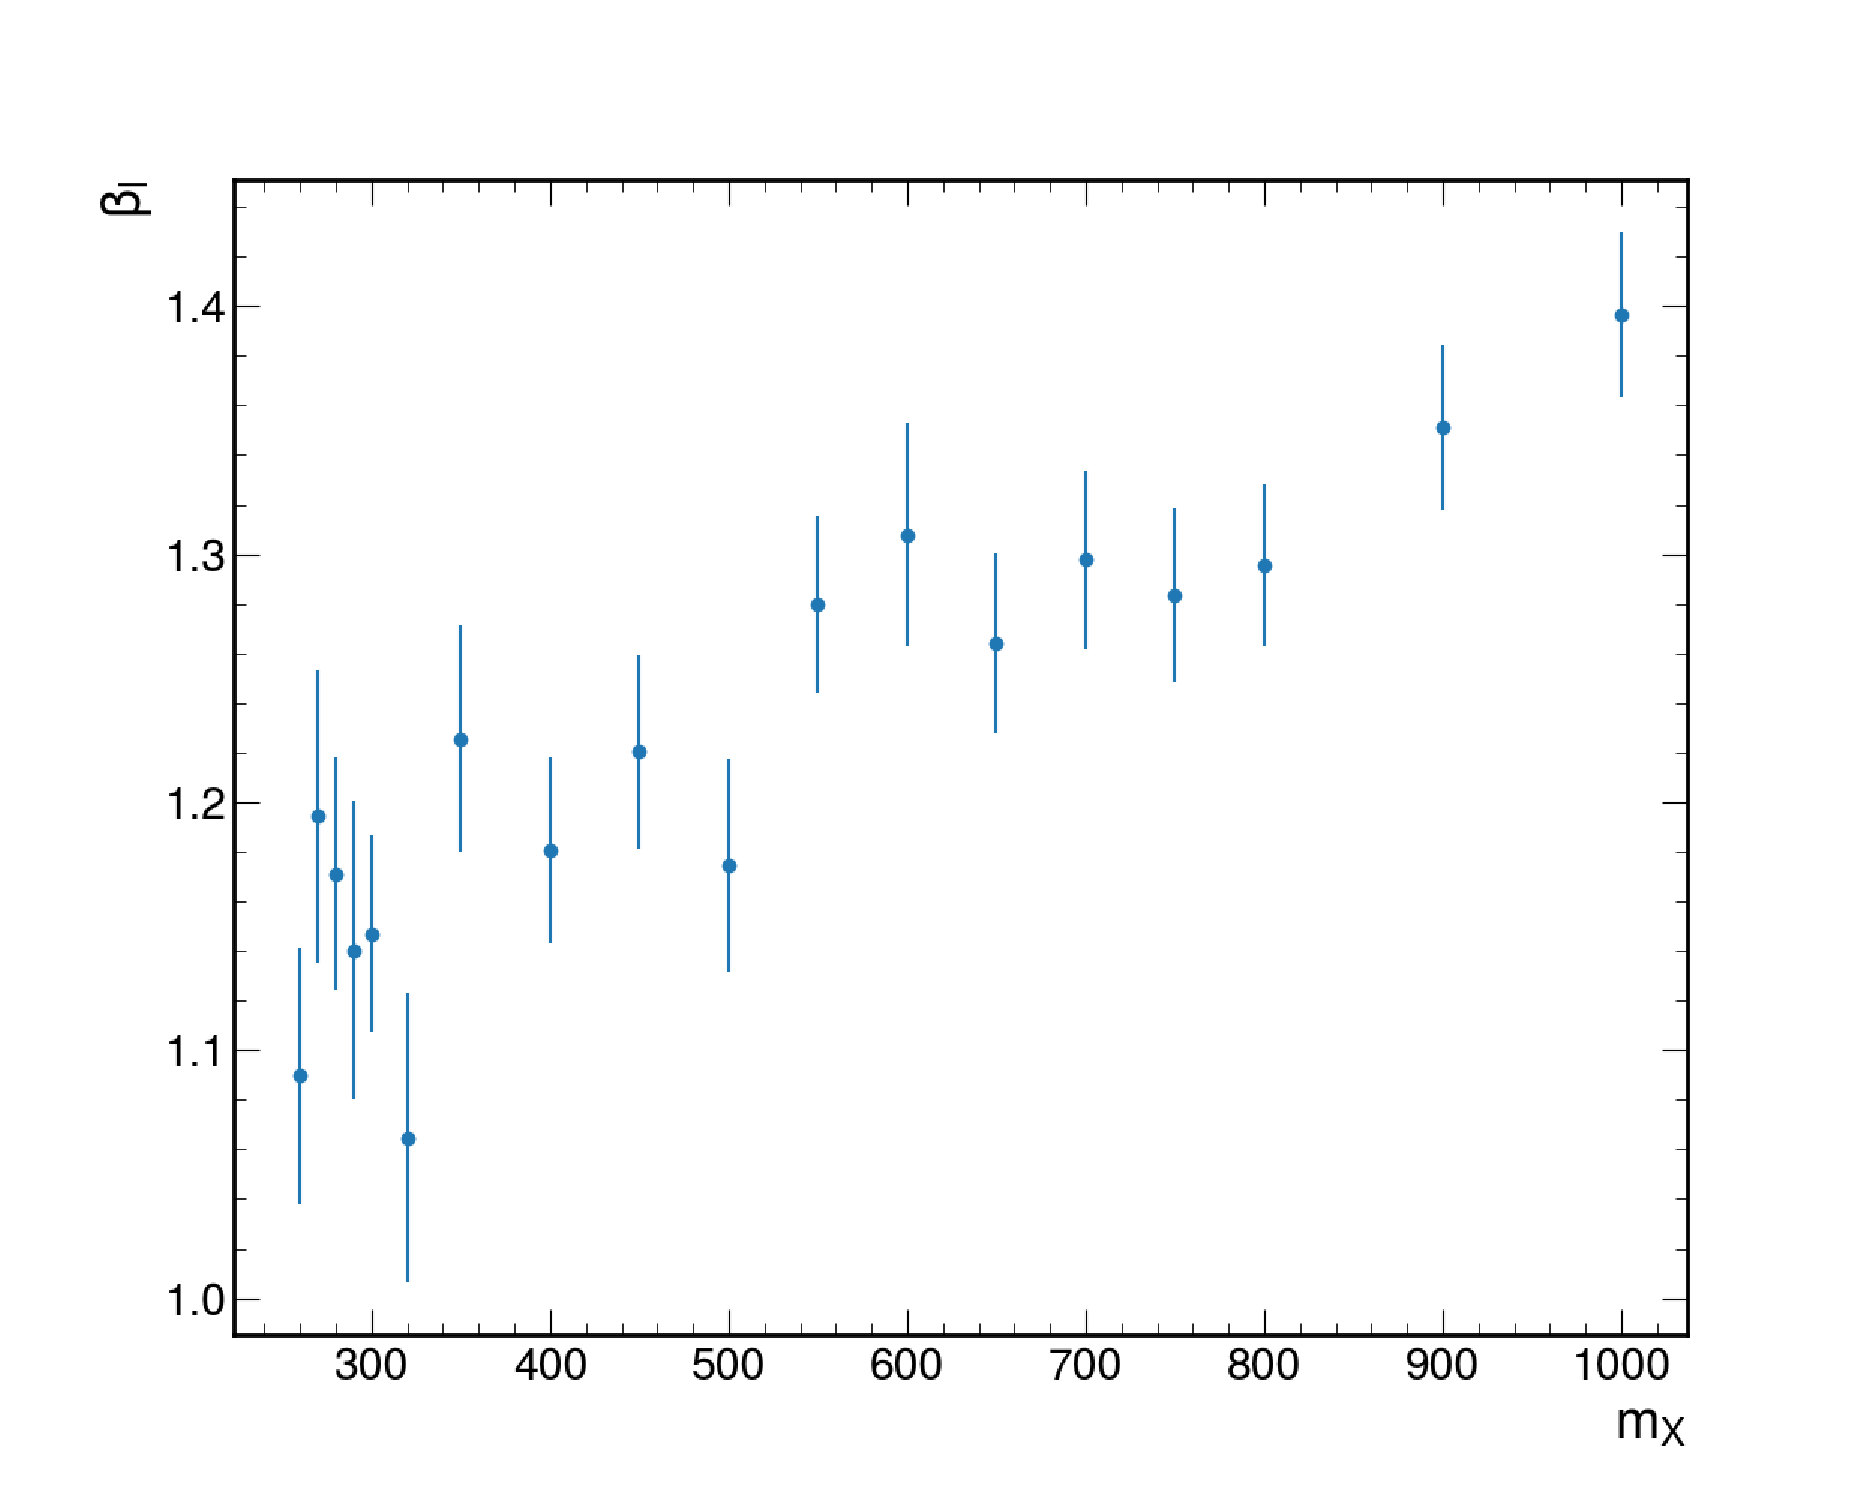
\includegraphics[width=0.49\textwidth]{Figures/Dihiggs/signal/shape_change/graviton_bl.pdf}
  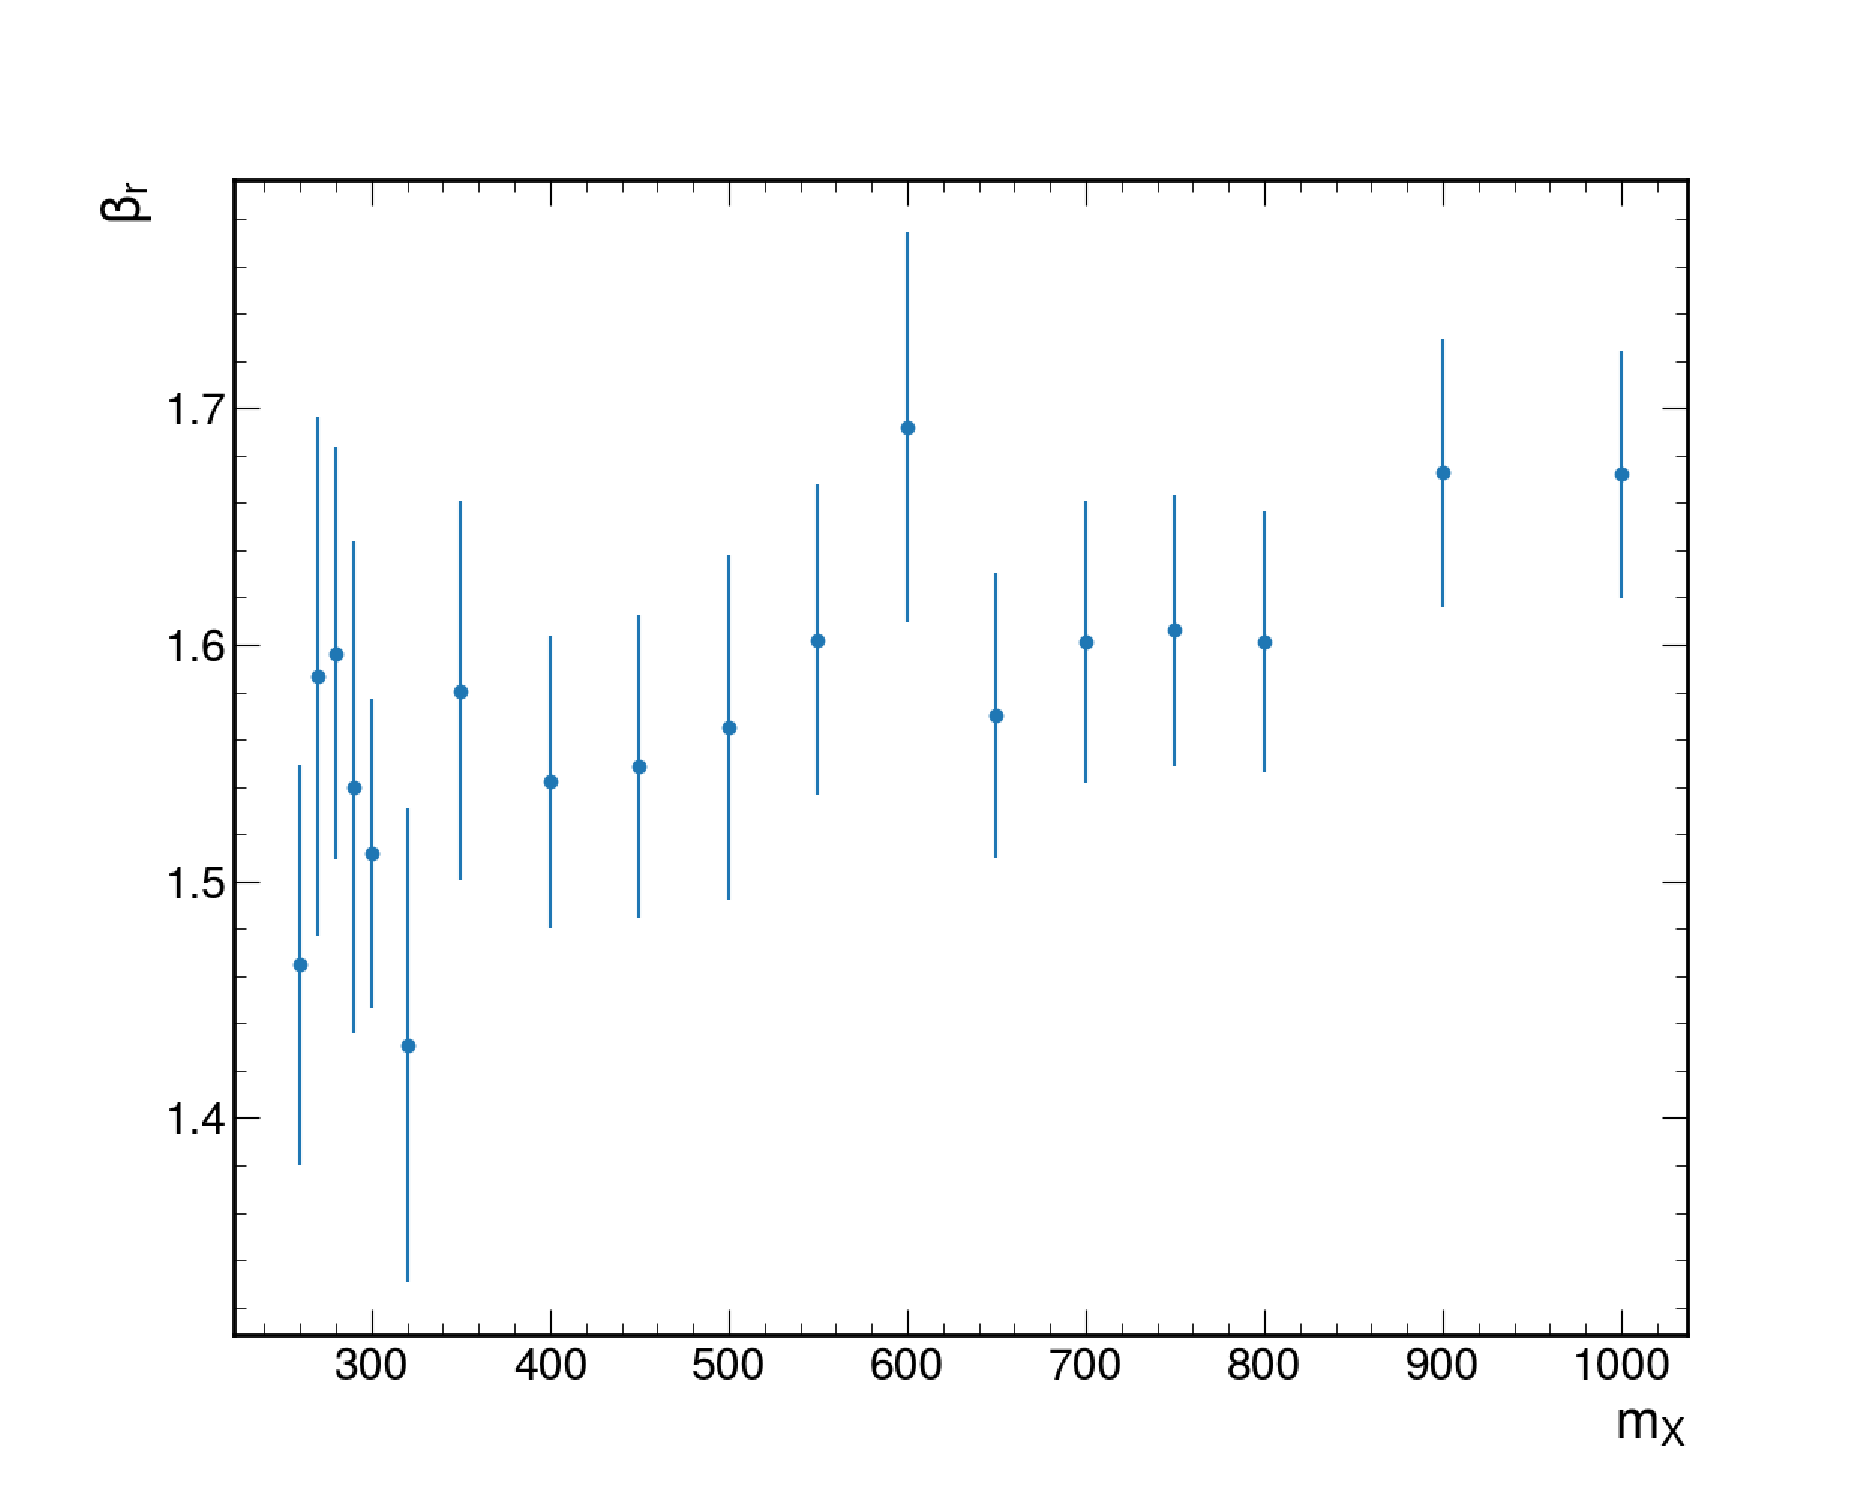
\includegraphics[width=0.49\textwidth]{Figures/Dihiggs/signal/shape_change/graviton_br.pdf} \\
  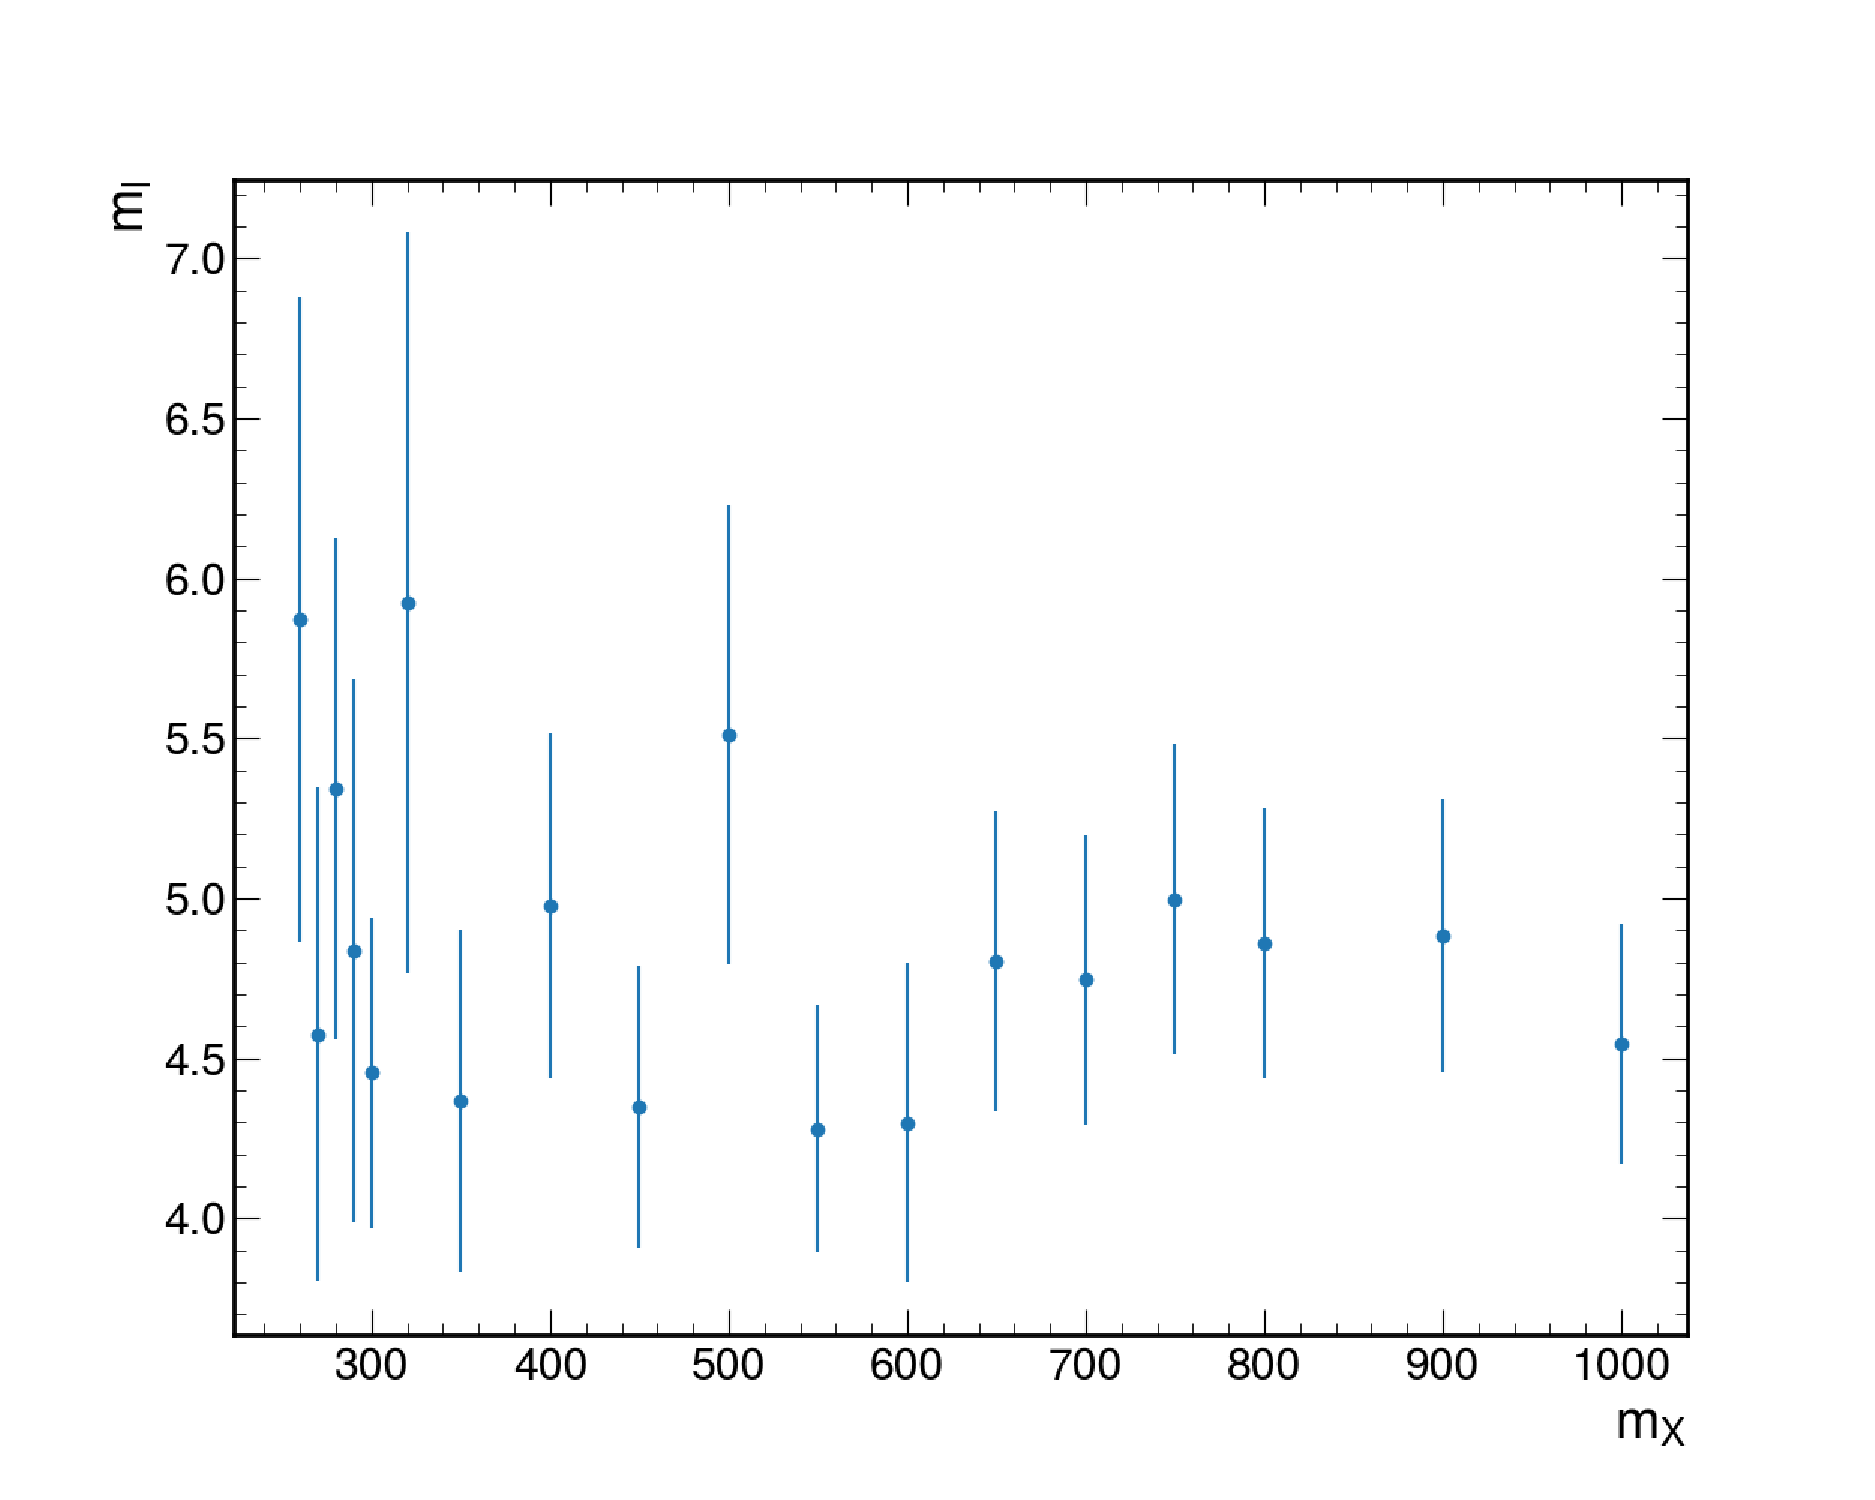
\includegraphics[width=0.49\textwidth]{Figures/Dihiggs/signal/shape_change/graviton_ml.pdf}
  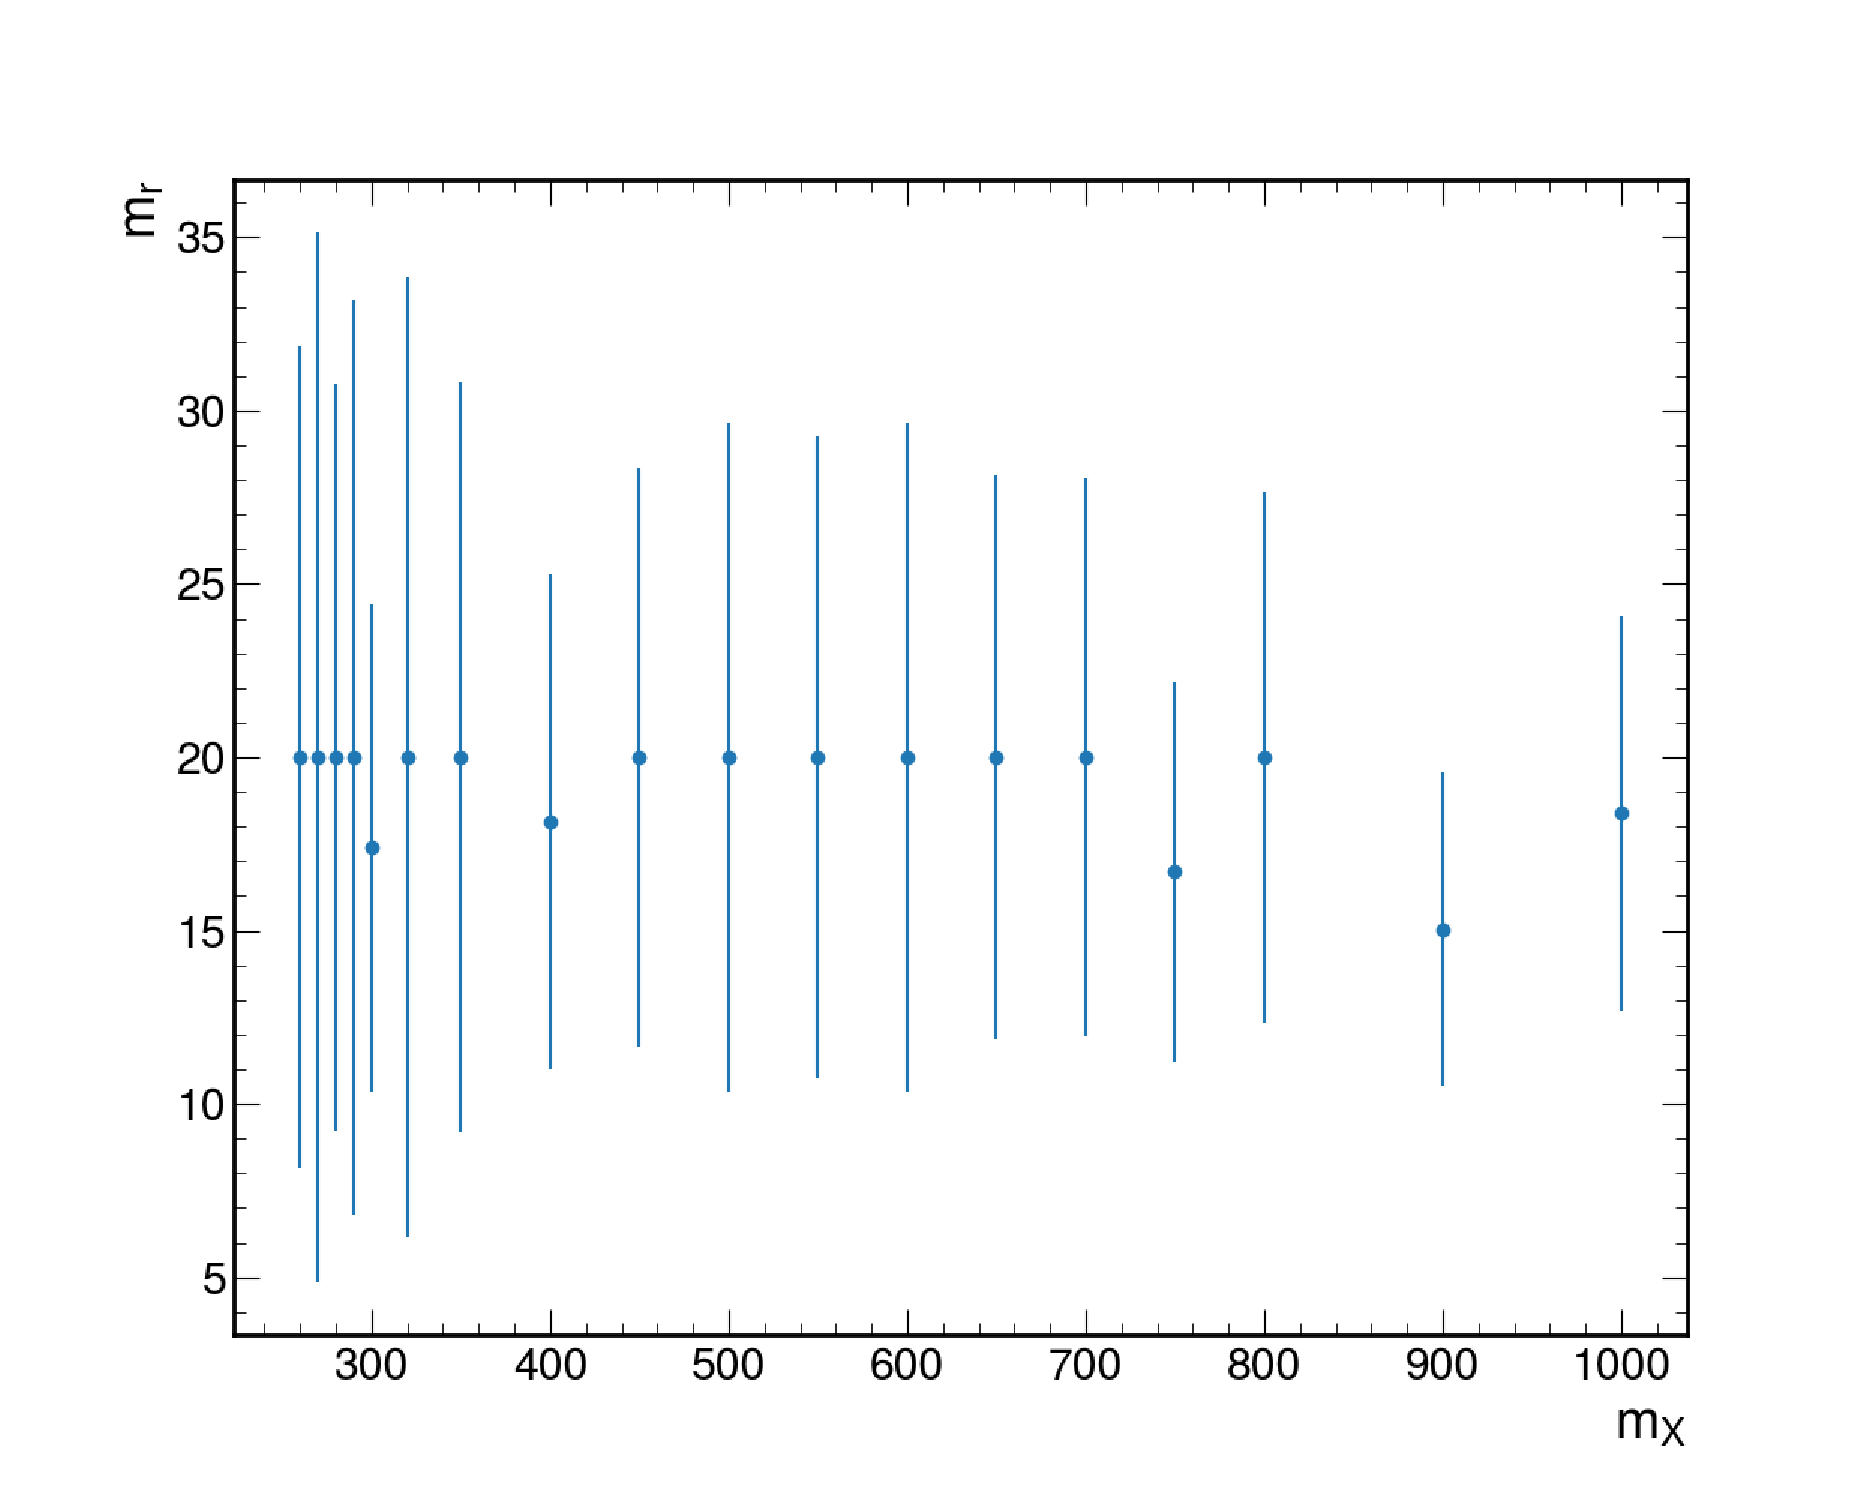
\includegraphics[width=0.49\textwidth]{Figures/Dihiggs/signal/shape_change/graviton_mr.pdf} 
  \caption[DCB Shape Parameters as a Function of \mX in the \XTwoHH Search]{Shape parameters from DCB fits to simulated \XTwoHH events, as a function of \mX. For each fit, a requirement of $\tilde{f}(\vec{x};m_X)>0.99$ is placed. The uncertainty in the shape parameters are indicated by the blue error bars.}\label{fig:graviton_shape_change}
\end{figure}

To validate the approach taken to determine the shape parameters, chosen nominal mass points are treated as intermediate mass points, and the interpolated shapes are compared to those found from a fit to the MC sample. These comparisons are shown in \cref{fig:shape_interpolation_check}. The goodness-of-fit using the interpolated shapes is still fair, validating the approach.

\begin{figure}
  \centering
  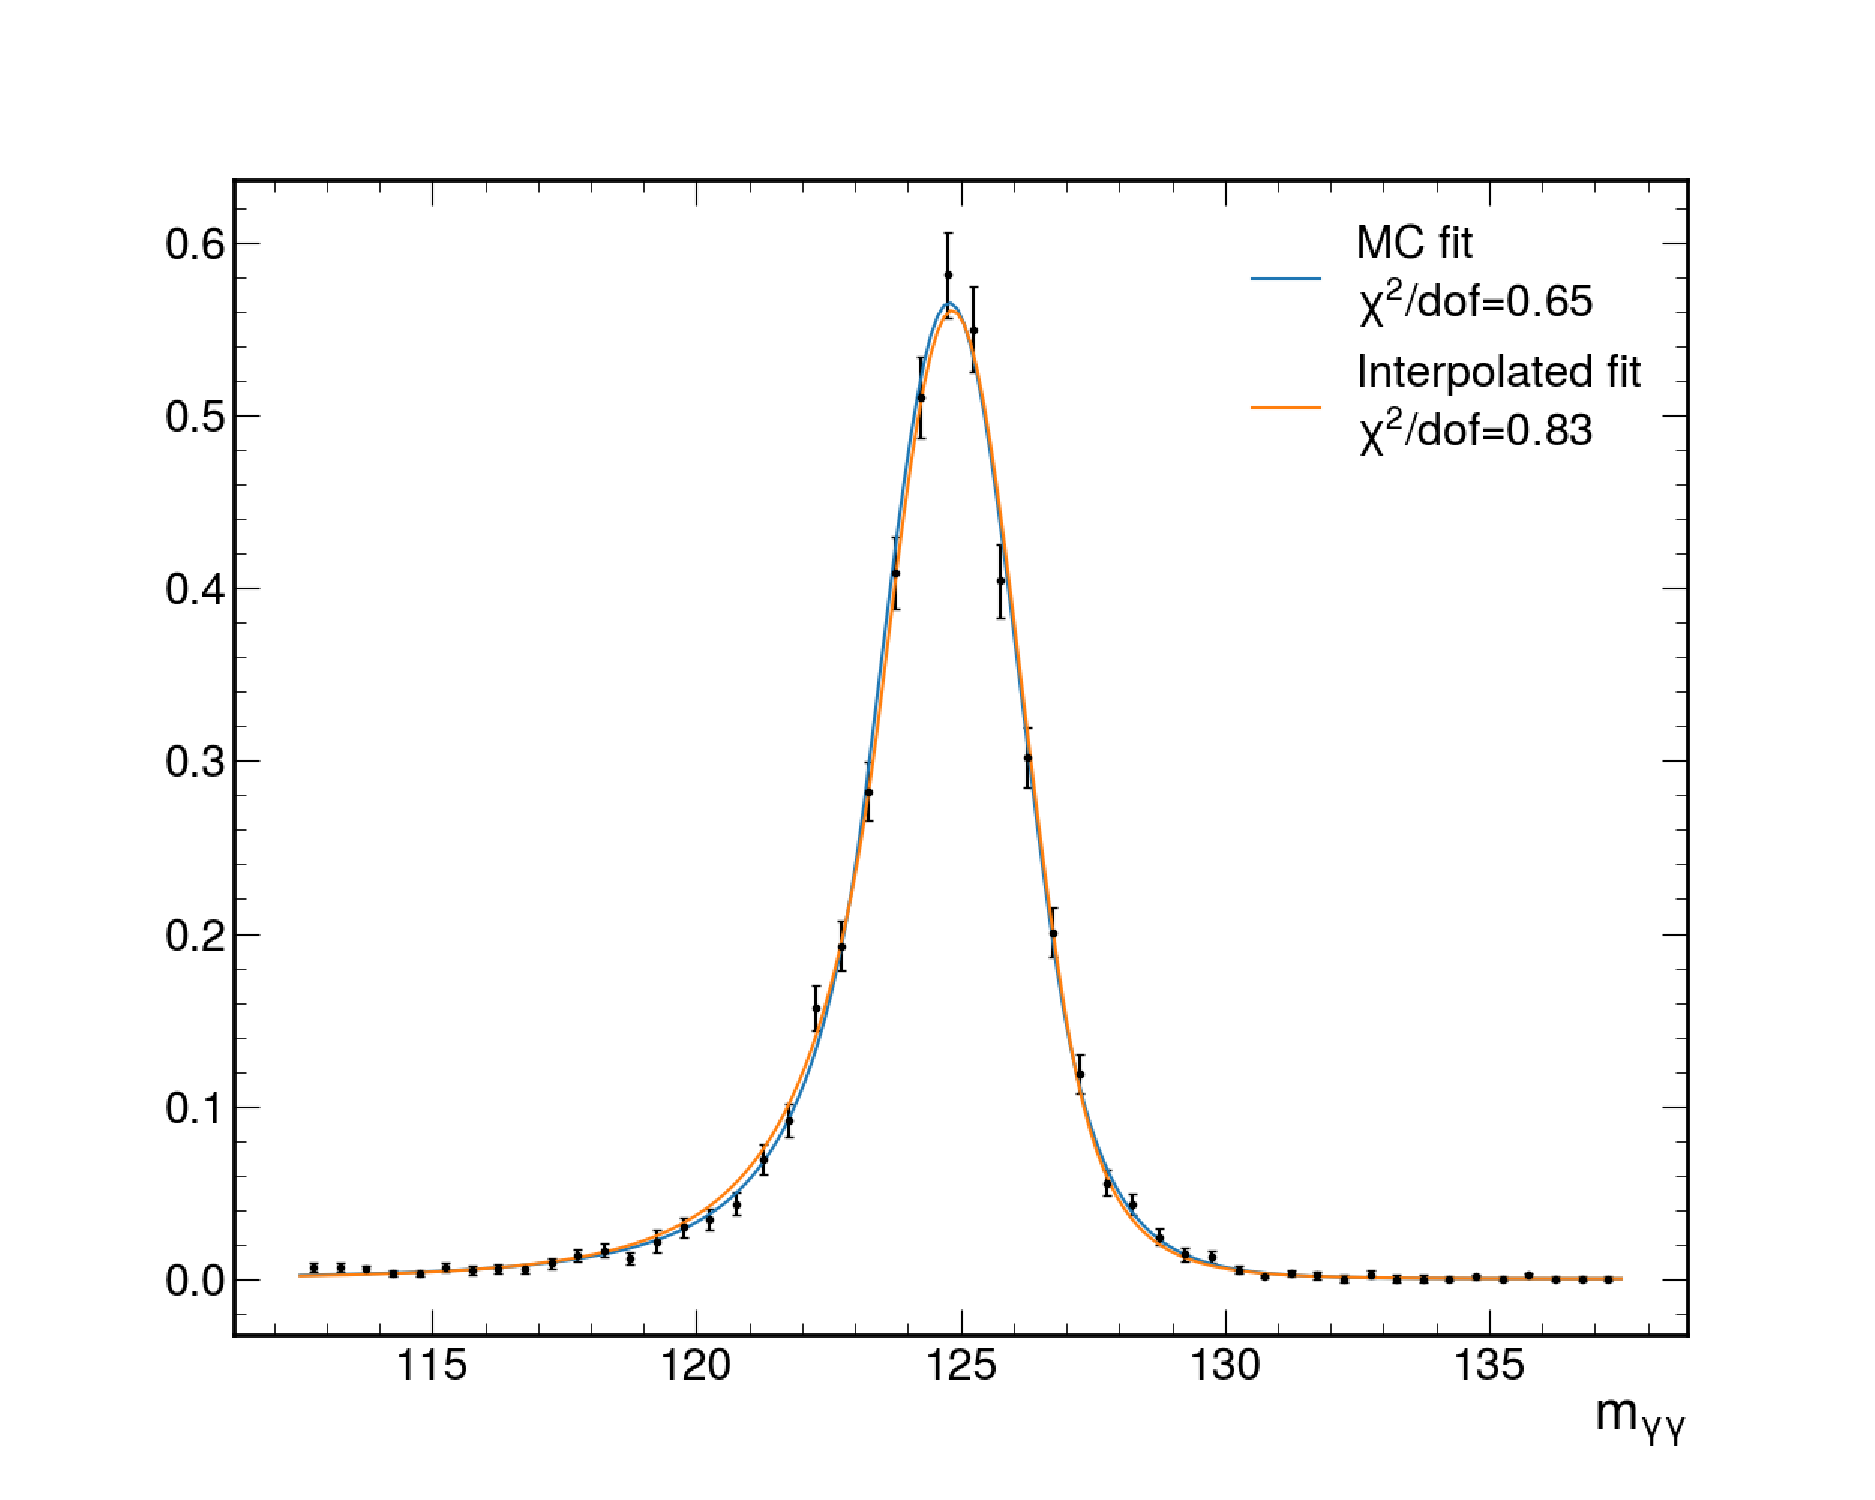
\includegraphics[width=0.49\textwidth]{Figures/Dihiggs/signal/interpolation_check/graviton/interpolation_check_270_125_2018_0.pdf}
  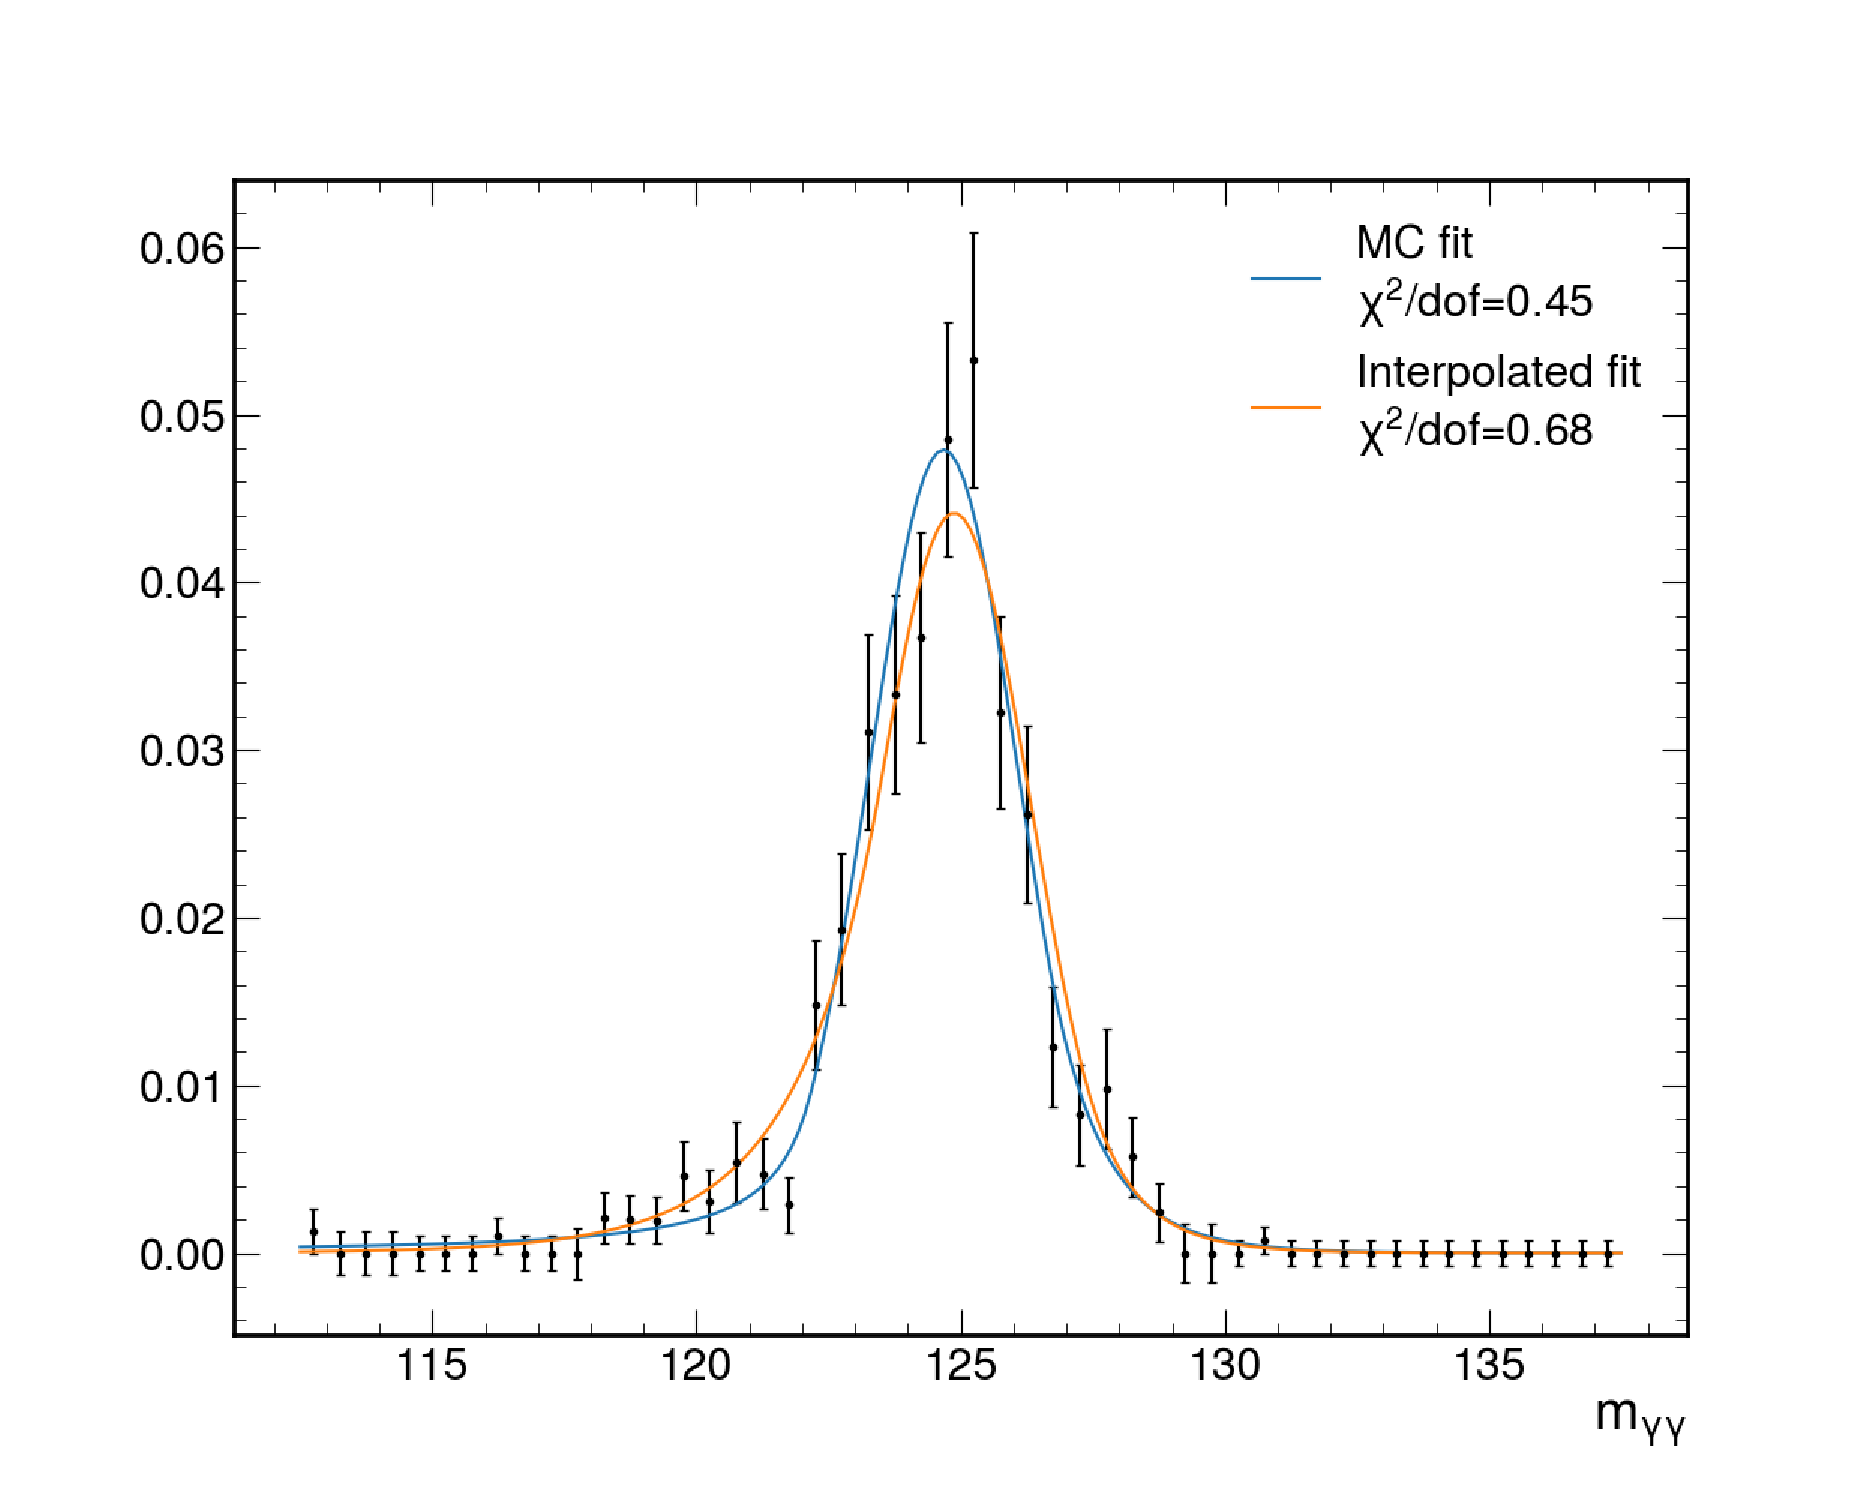
\includegraphics[width=0.49\textwidth]{Figures/Dihiggs/signal/interpolation_check/graviton/interpolation_check_270_125_2018_1.pdf} \\
  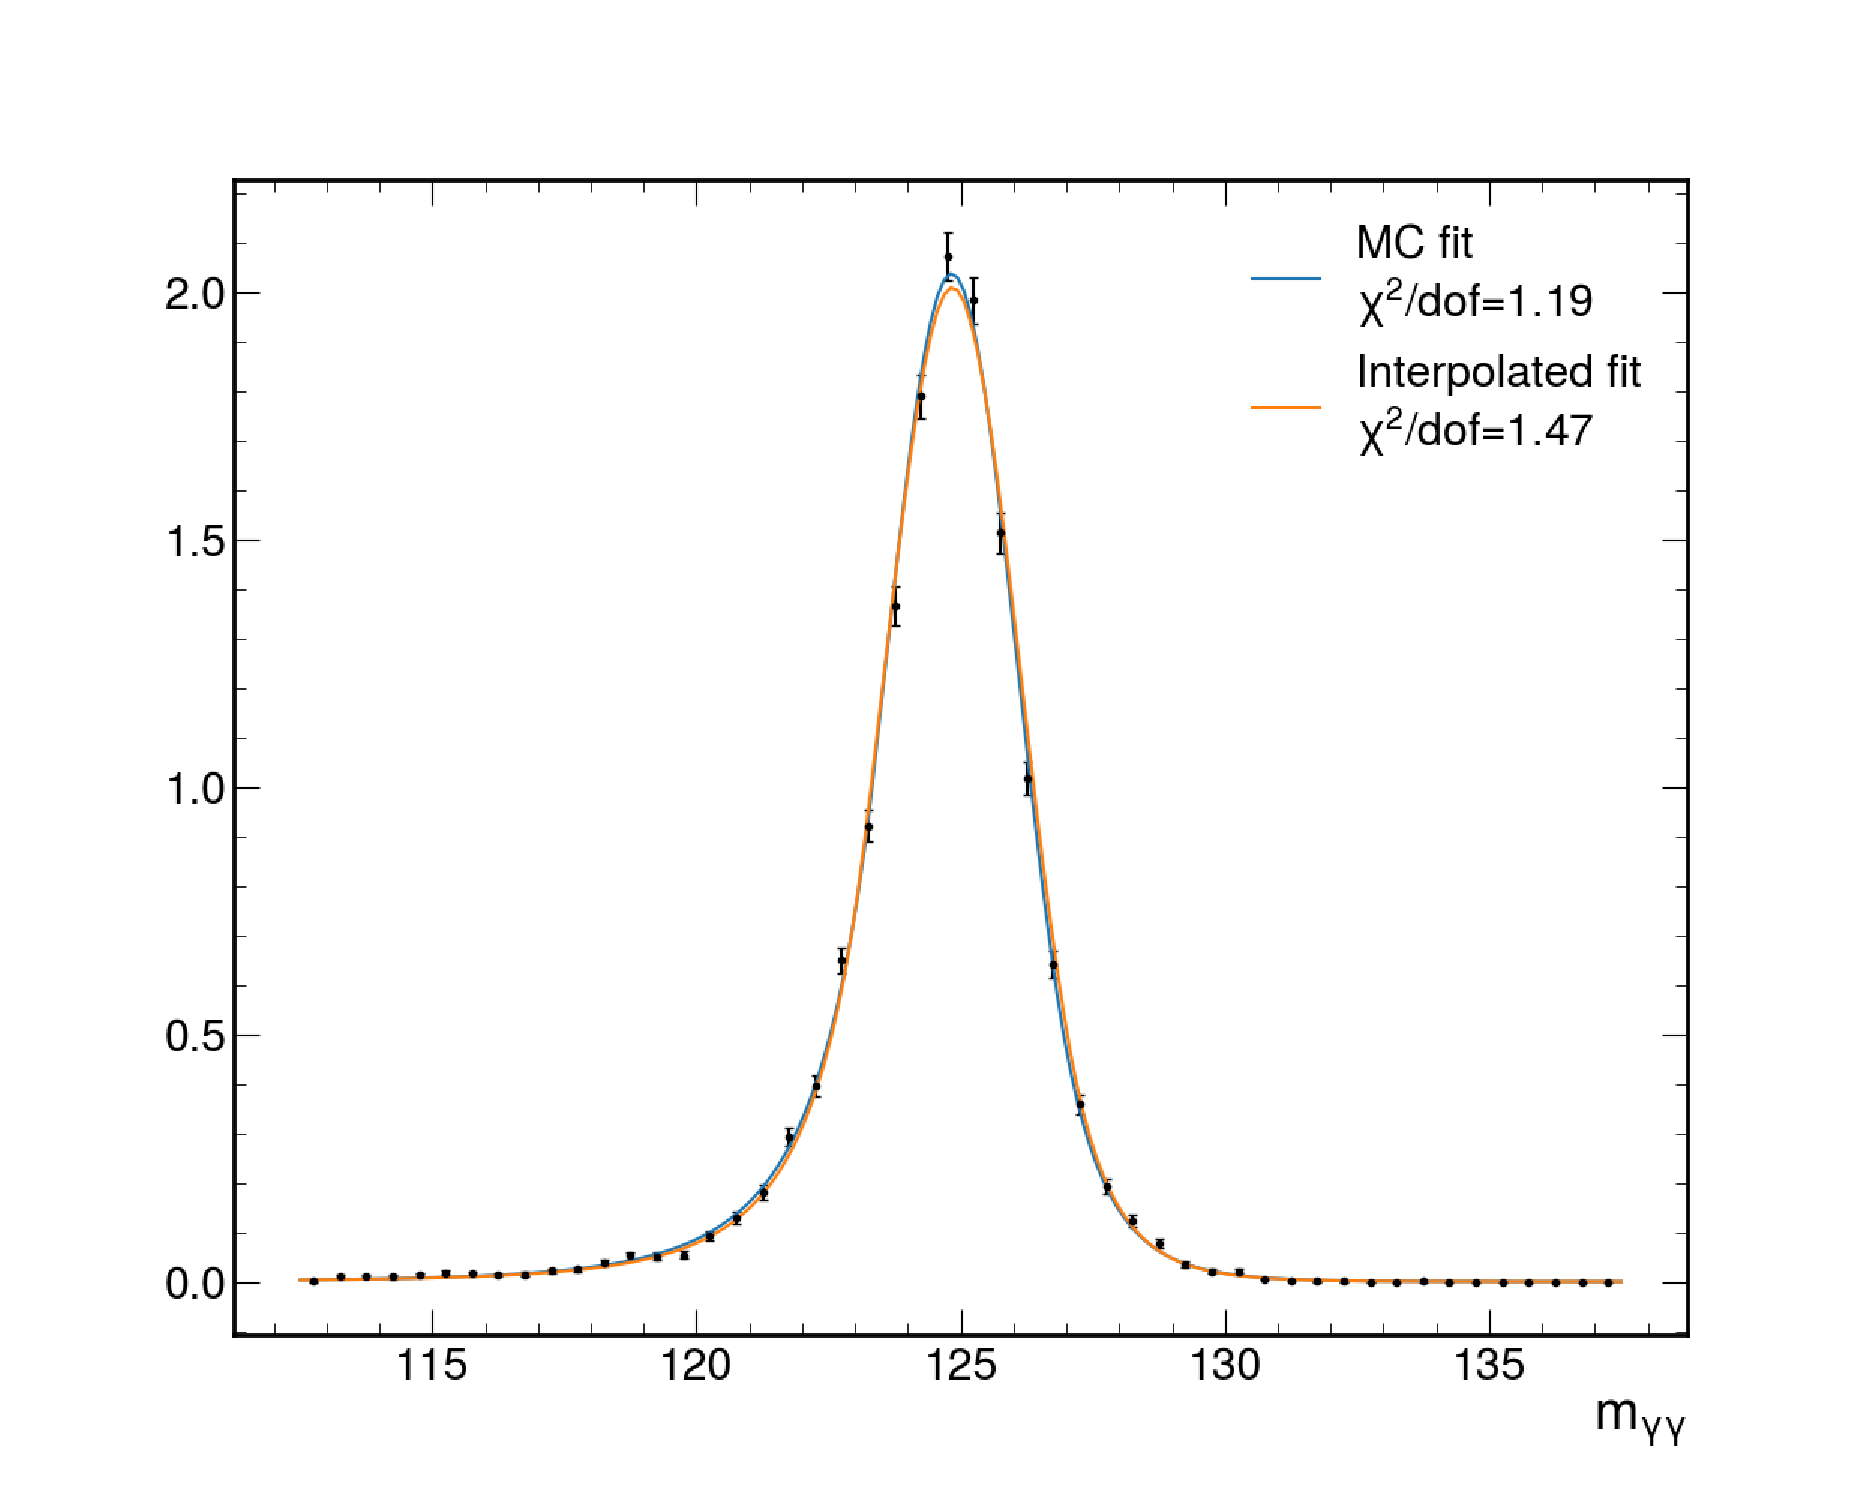
\includegraphics[width=0.49\textwidth]{Figures/Dihiggs/signal/interpolation_check/graviton/interpolation_check_500_125_2018_0.pdf}
  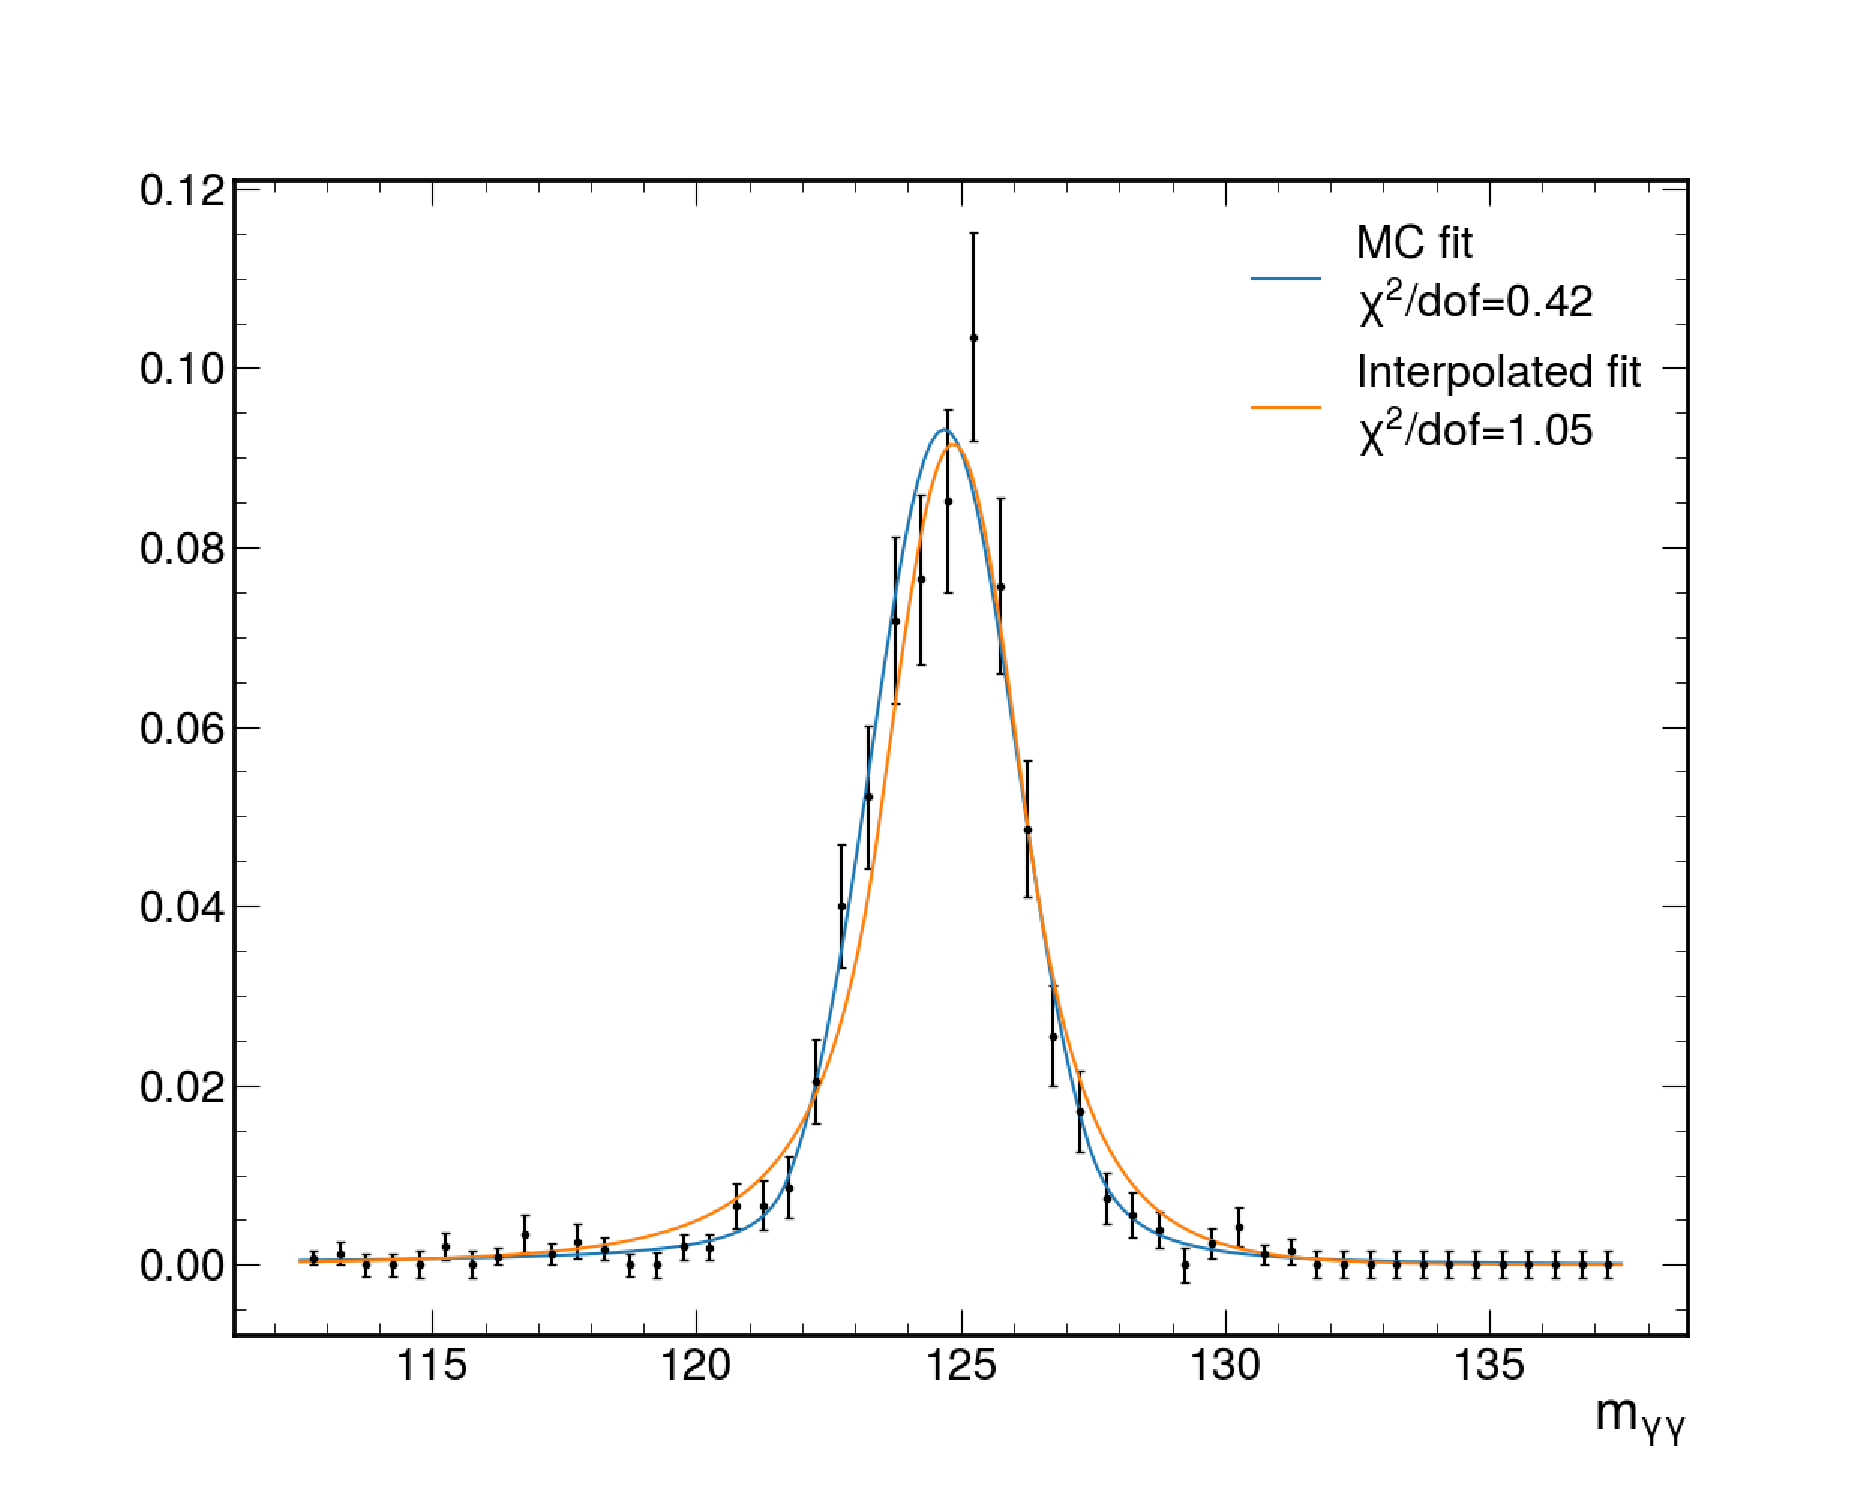
\includegraphics[width=0.49\textwidth]{Figures/Dihiggs/signal/interpolation_check/graviton/interpolation_check_500_125_2018_1.pdf} \\
  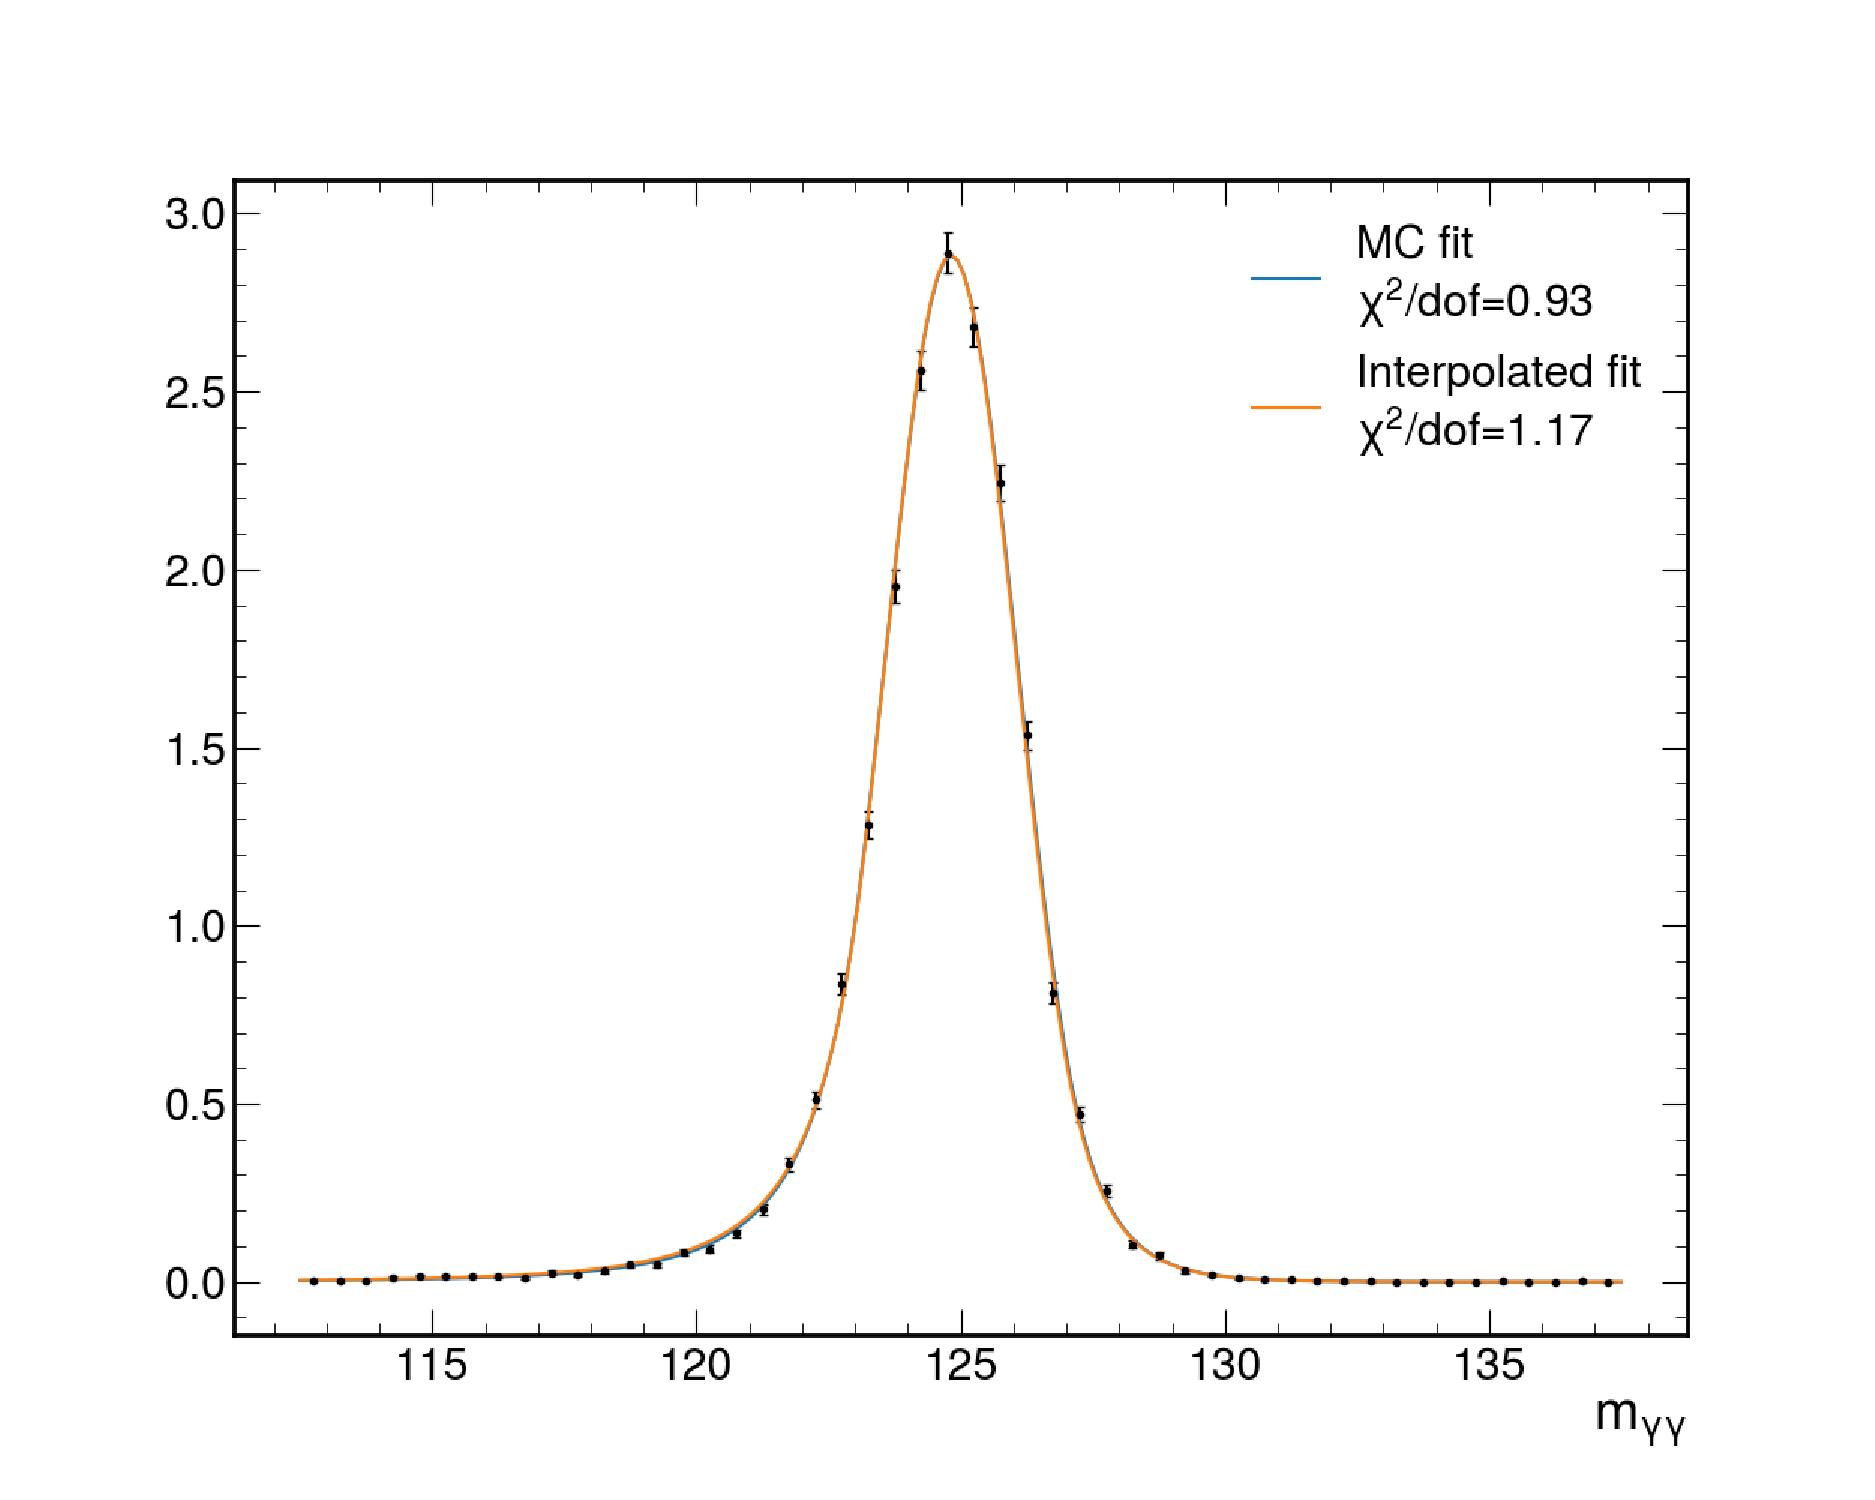
\includegraphics[width=0.49\textwidth]{Figures/Dihiggs/signal/interpolation_check/graviton/interpolation_check_700_125_2018_0.pdf}
  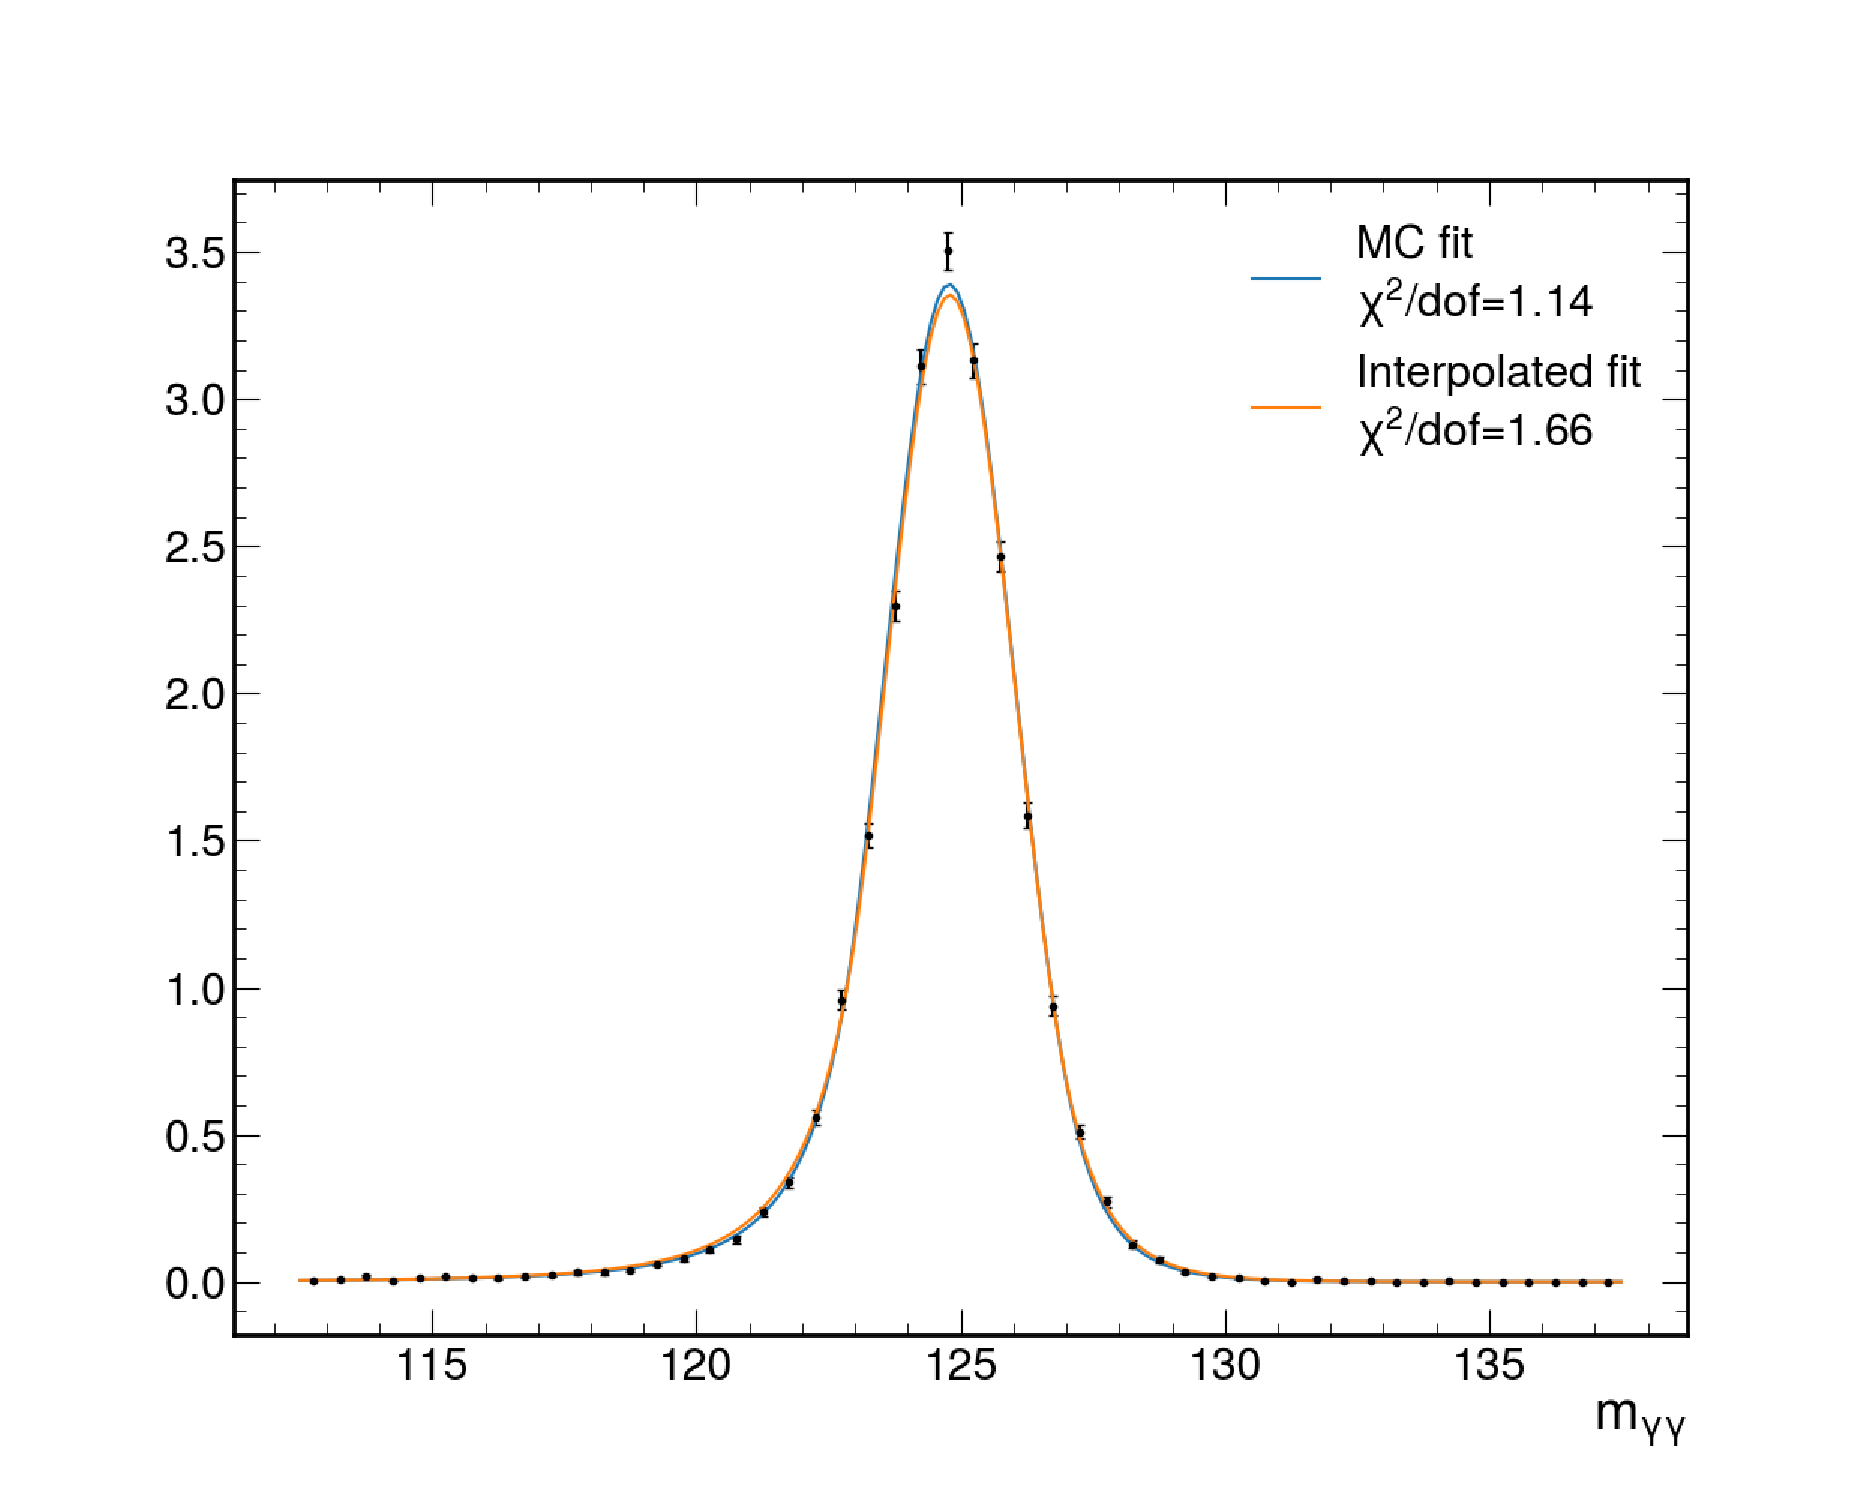
\includegraphics[width=0.49\textwidth]{Figures/Dihiggs/signal/interpolation_check/graviton/interpolation_check_900_125_2018_0.pdf} \\
  \caption[Validation of Shape Parameter Interpolation]{Comparisons between signal models derived via direct fits to MC events and derived via the interpolation procedure which uses fits to MC events at neighbouring mass points. All comparisons are for the \XTwoHH analysis in 2018. To isolate the comparison to the shape interpolation, the signal efficiency of the interpolated model is set to the value from the direct fit. The top and middle plots show the $\mX=270$ and 500\GeV mass points respectively where the left and right plots are for category 0 and category 1 respectively. The bottom-left and bottom-right plots are for category 0 for the $\mX=700$ and 900\GeV mass points respectively.}\label{fig:shape_interpolation_check}
\end{figure}

In the \XYH searches, $\epsilon$ and $\vec{\Psi}$ must be studied as a function of \mY as well. \Cref{fig:sigeff_change_2d} shows $\epsilon$ as a function of \mY when $\mX=1000$\GeV for the \XYttHgg and high-mass \XYggHtt searches, and \cref{fig:shape_change_y_gg_high_mass_my} similarly shows the dependence of the shape parameters on \mY in the high-mass \XYggHtt search. These figures lead to the same conclusions as for the \XHH searches. The parameters: $\epsilon$, $\Delta\mgg$, $\sigma$, and $\beta_l$ must be interpolated, now as functions of \mX and \mY, and the $\beta_r$, $m_l$ and $m_r$ parameters are taken from the closest nominal mass point. The 2D splines are implemented using the \SCIPY package~\cite{2020SciPy-NMeth} where the cubic spline uses techniques described in Ref.~\cite{ALFELD1984169}. To illustrate how these splines work in 2D, a linear and cubic spline for an arbitrary function is shown in \cref{fig:2d_interp_toy_example}. The choice of the type of spline, and the derivation of the systematic uncertainty, is the same as for the 1D splines. 

\begin{figure}
  \centering
  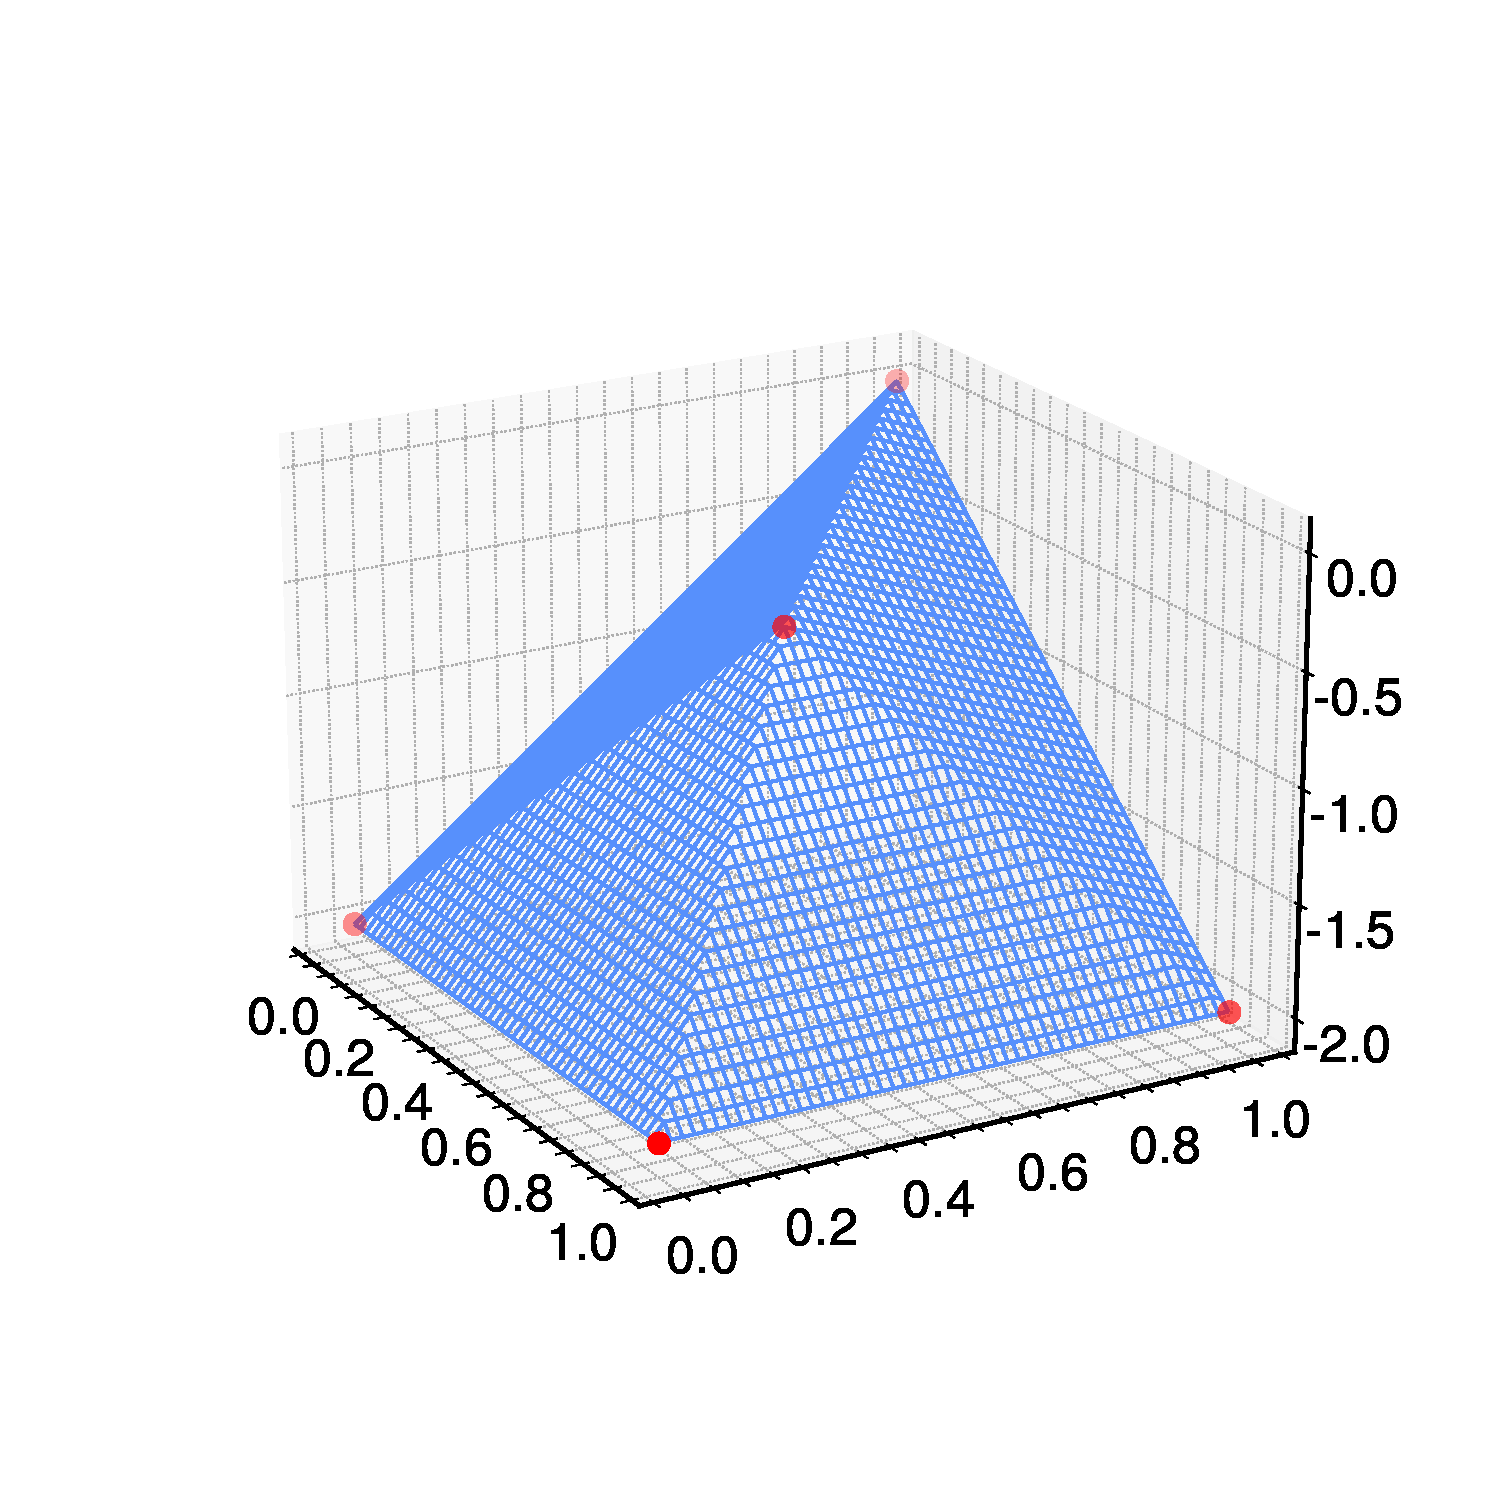
\includegraphics[width=0.49\textwidth]{Figures/Dihiggs/interp_toy_linear.pdf}
  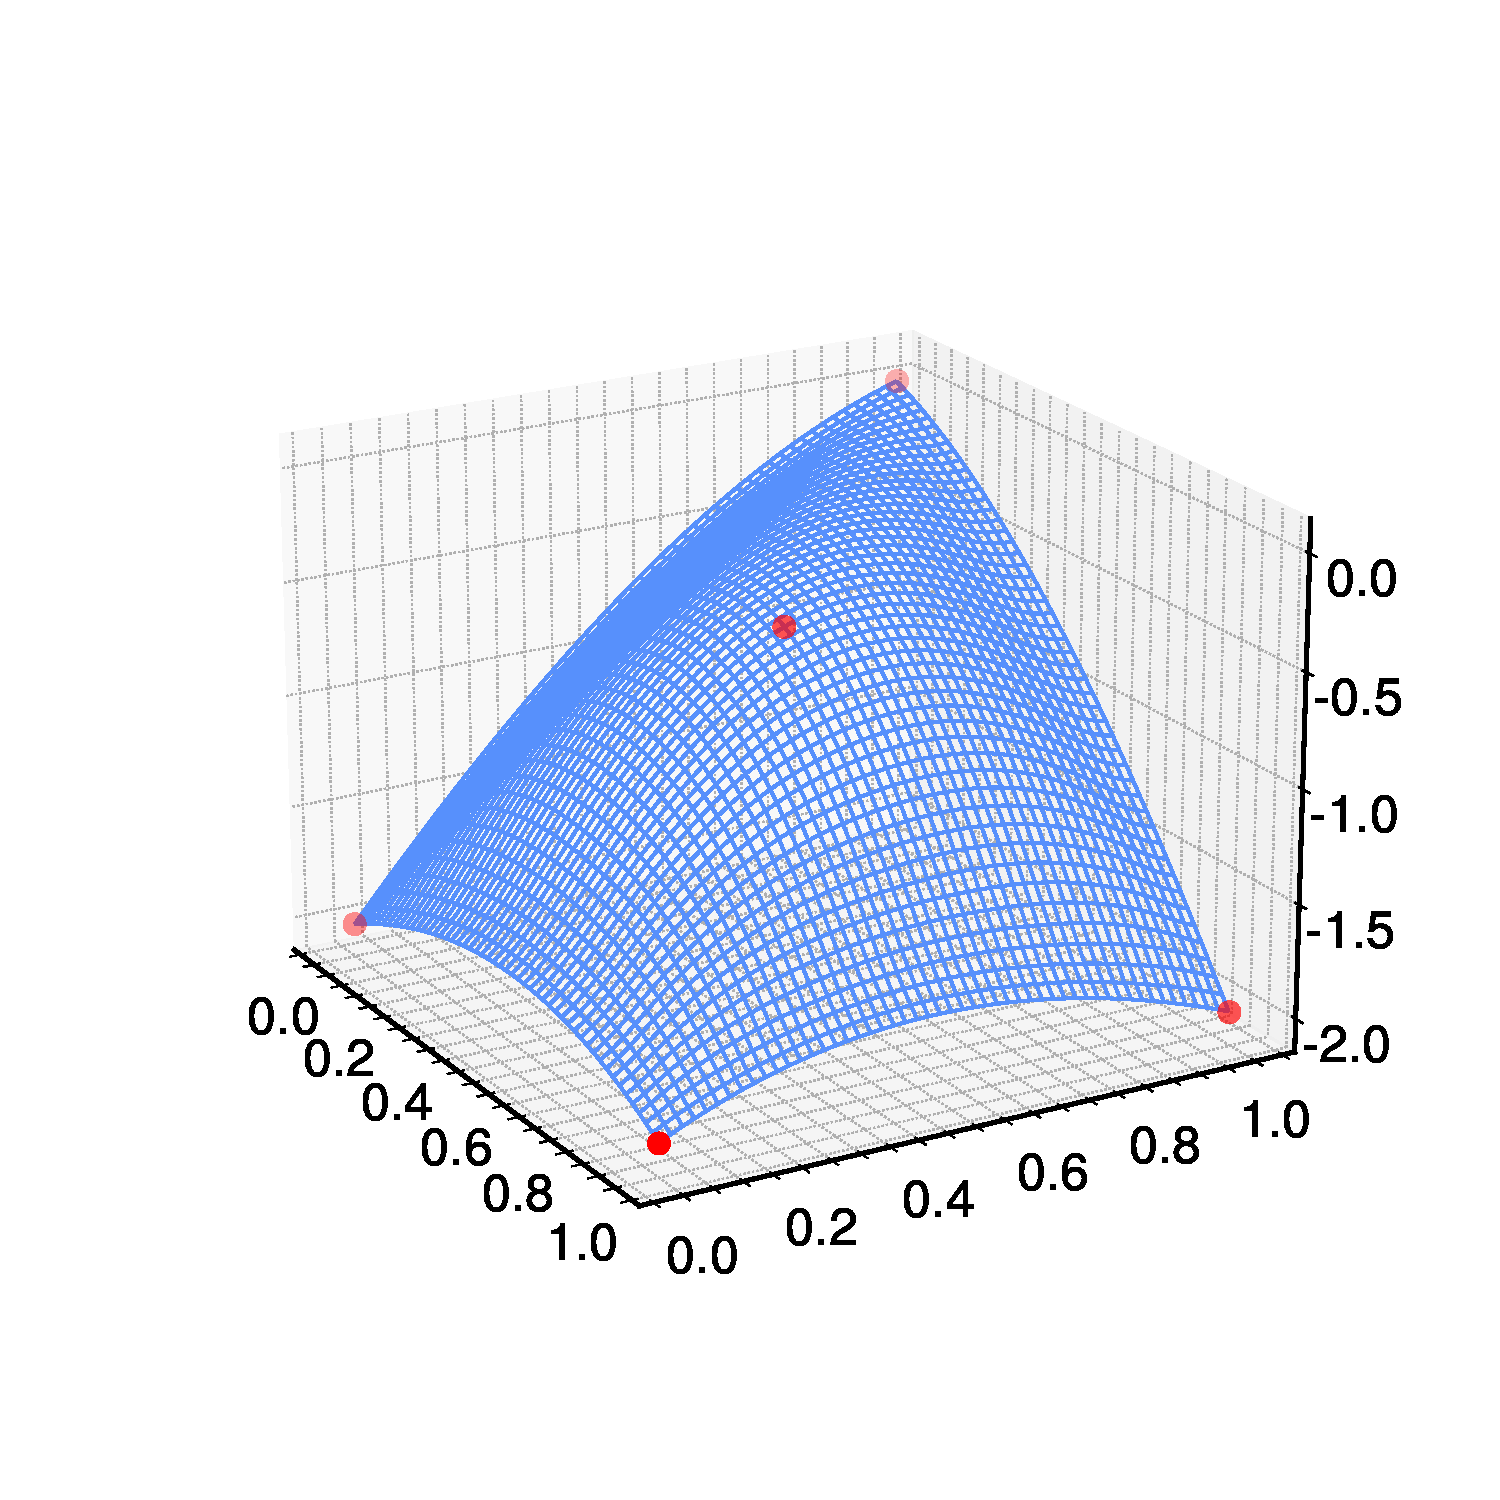
\includegraphics[width=0.49\textwidth]{Figures/Dihiggs/interp_toy_cubic.pdf}
  \caption[Toy Examples of Linear and Cubic Interpolation in 2D]{Examples of linear (left) and cubic (right) interpolation for an arbitrary function in two dimensions.}\label{fig:2d_interp_toy_example}
\end{figure}

\begin{figure}
  \centering
  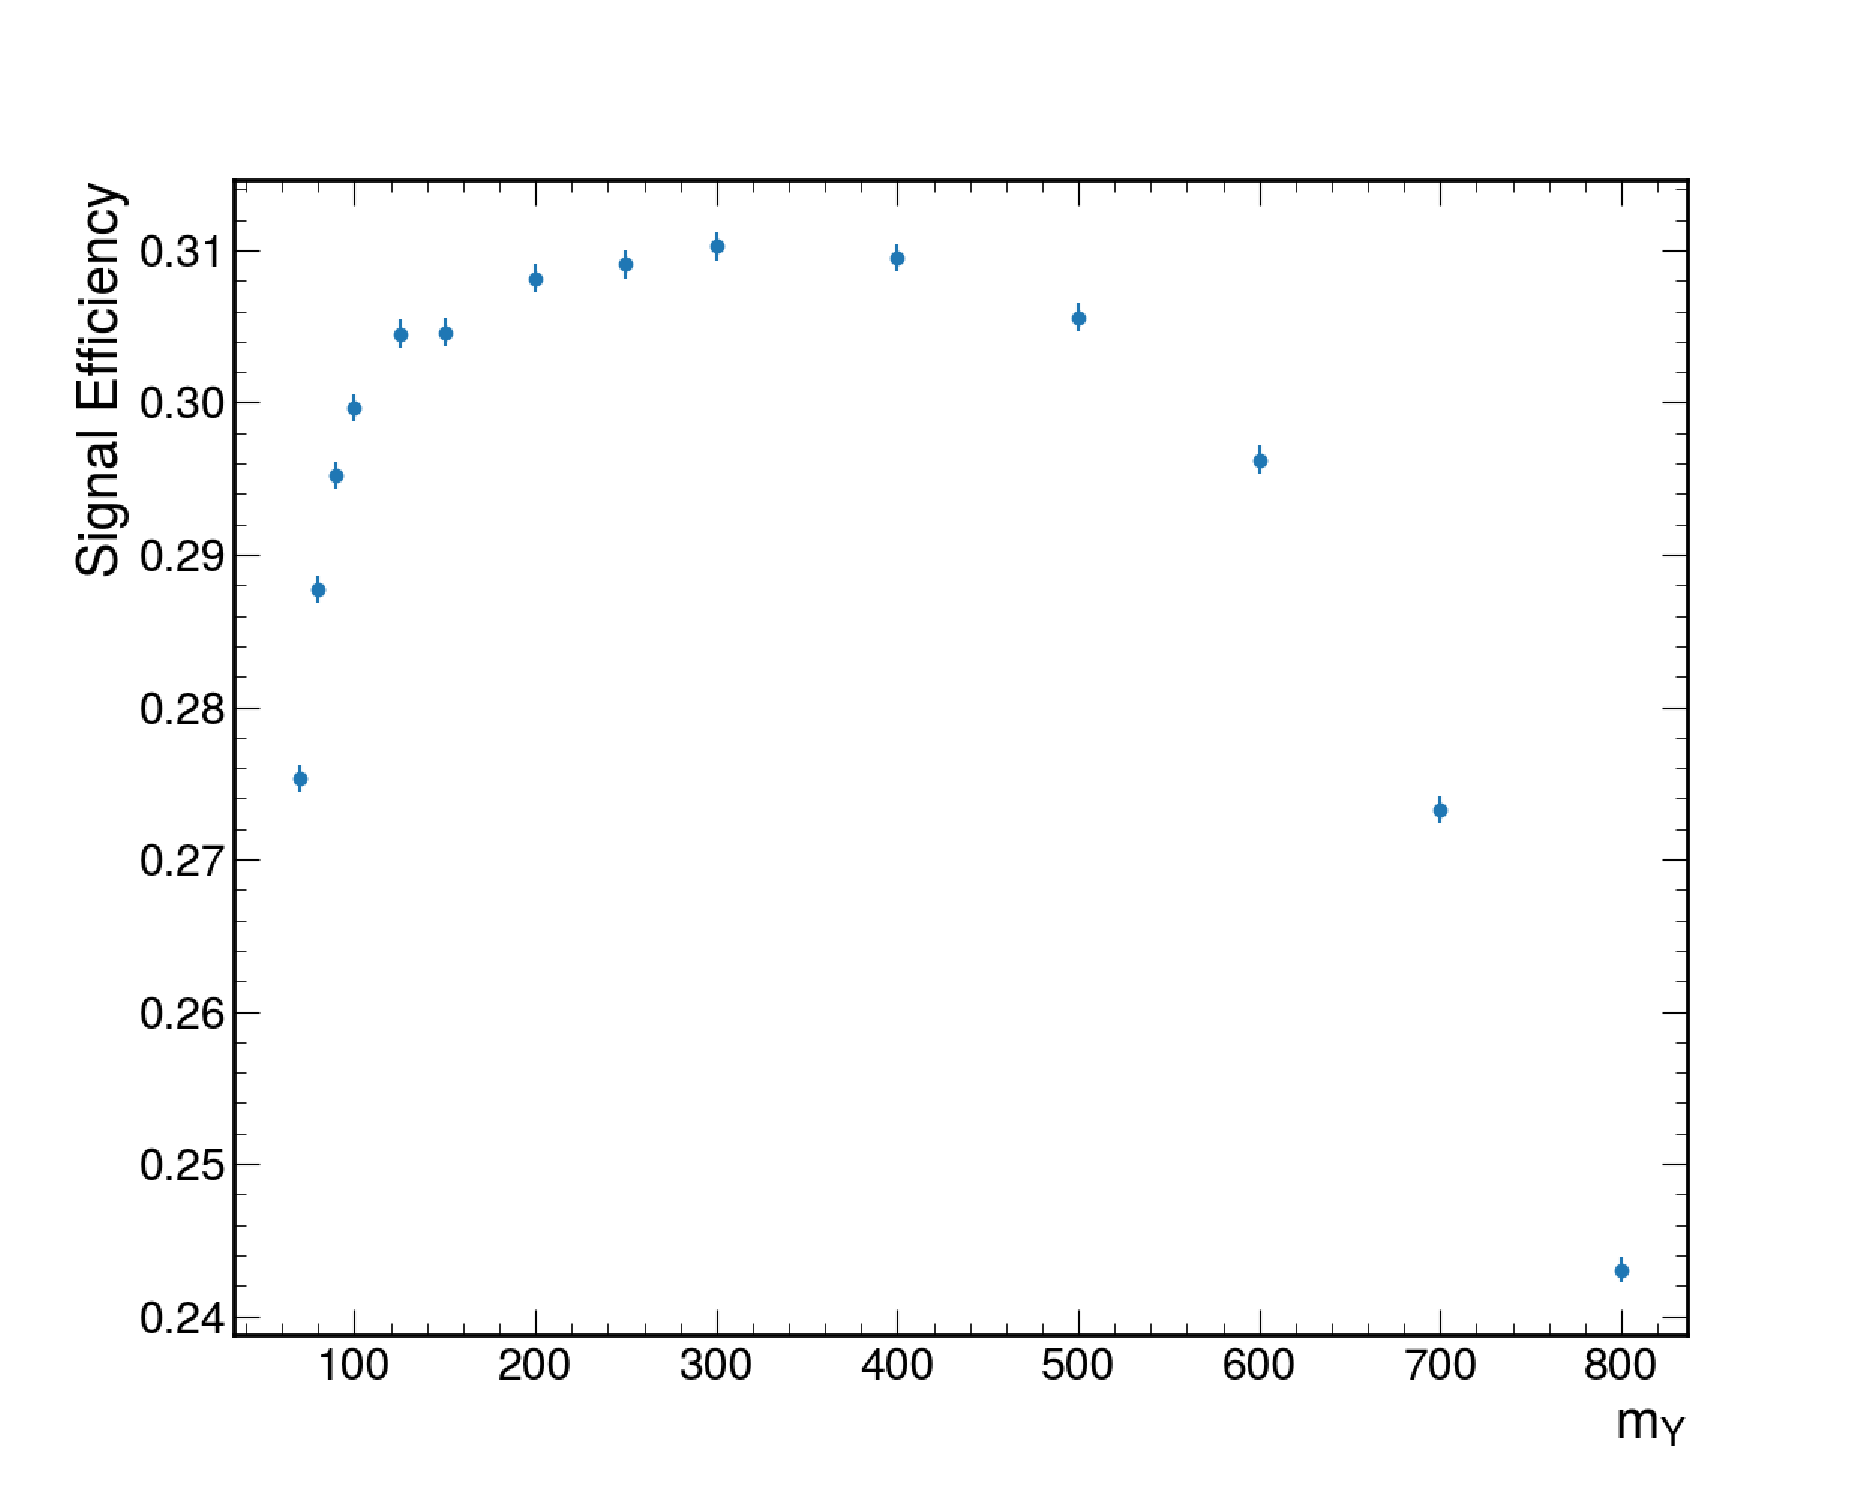
\includegraphics[width=0.49\textwidth]{Figures/Dihiggs/signal/shape_change/y_tautau_sigeff.pdf}
  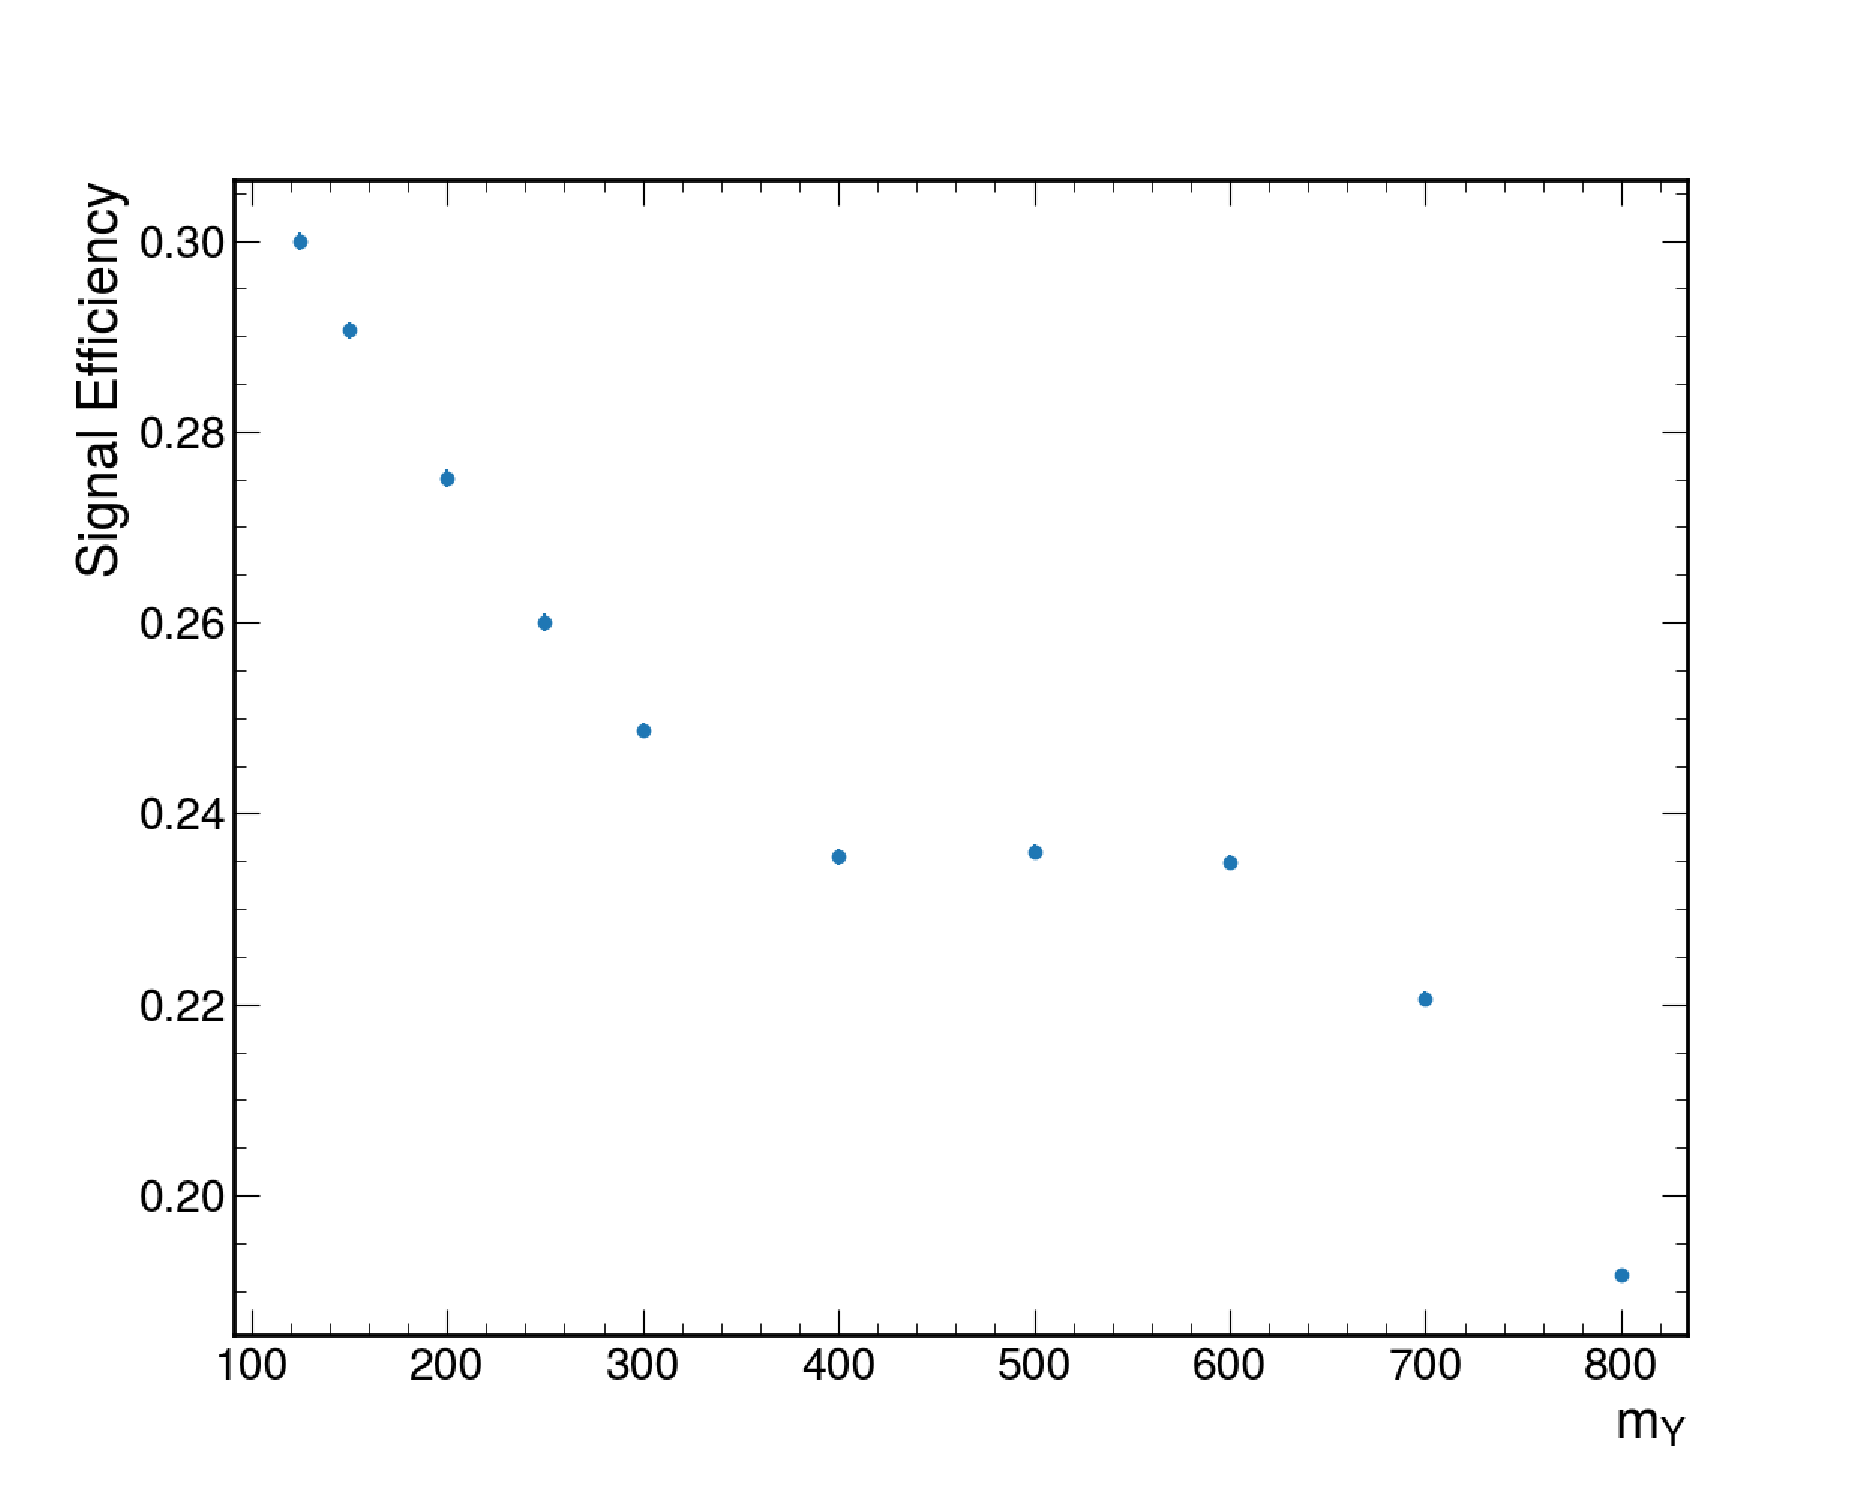
\includegraphics[width=0.49\textwidth]{Figures/Dihiggs/signal/shape_change/y_gg_high_mass_my_sigeff.pdf}
  \caption[Signal Efficiency as a Function of \mY in the \XYH Searches]{Signal efficiency as a function of \mY where $\mX=1000$\GeV for the \XYttHgg (left) and high-mass \XYttHgg (right) searches. These models are derived from MC across all years with a requirement on the pNN score of $\tilde{f}(\vec{x};m_X,m_Y)>0.99$ placed which is representative of the purest categories in the analysis.}\label{fig:sigeff_change_2d}
\end{figure}

\begin{figure}
  \centering
  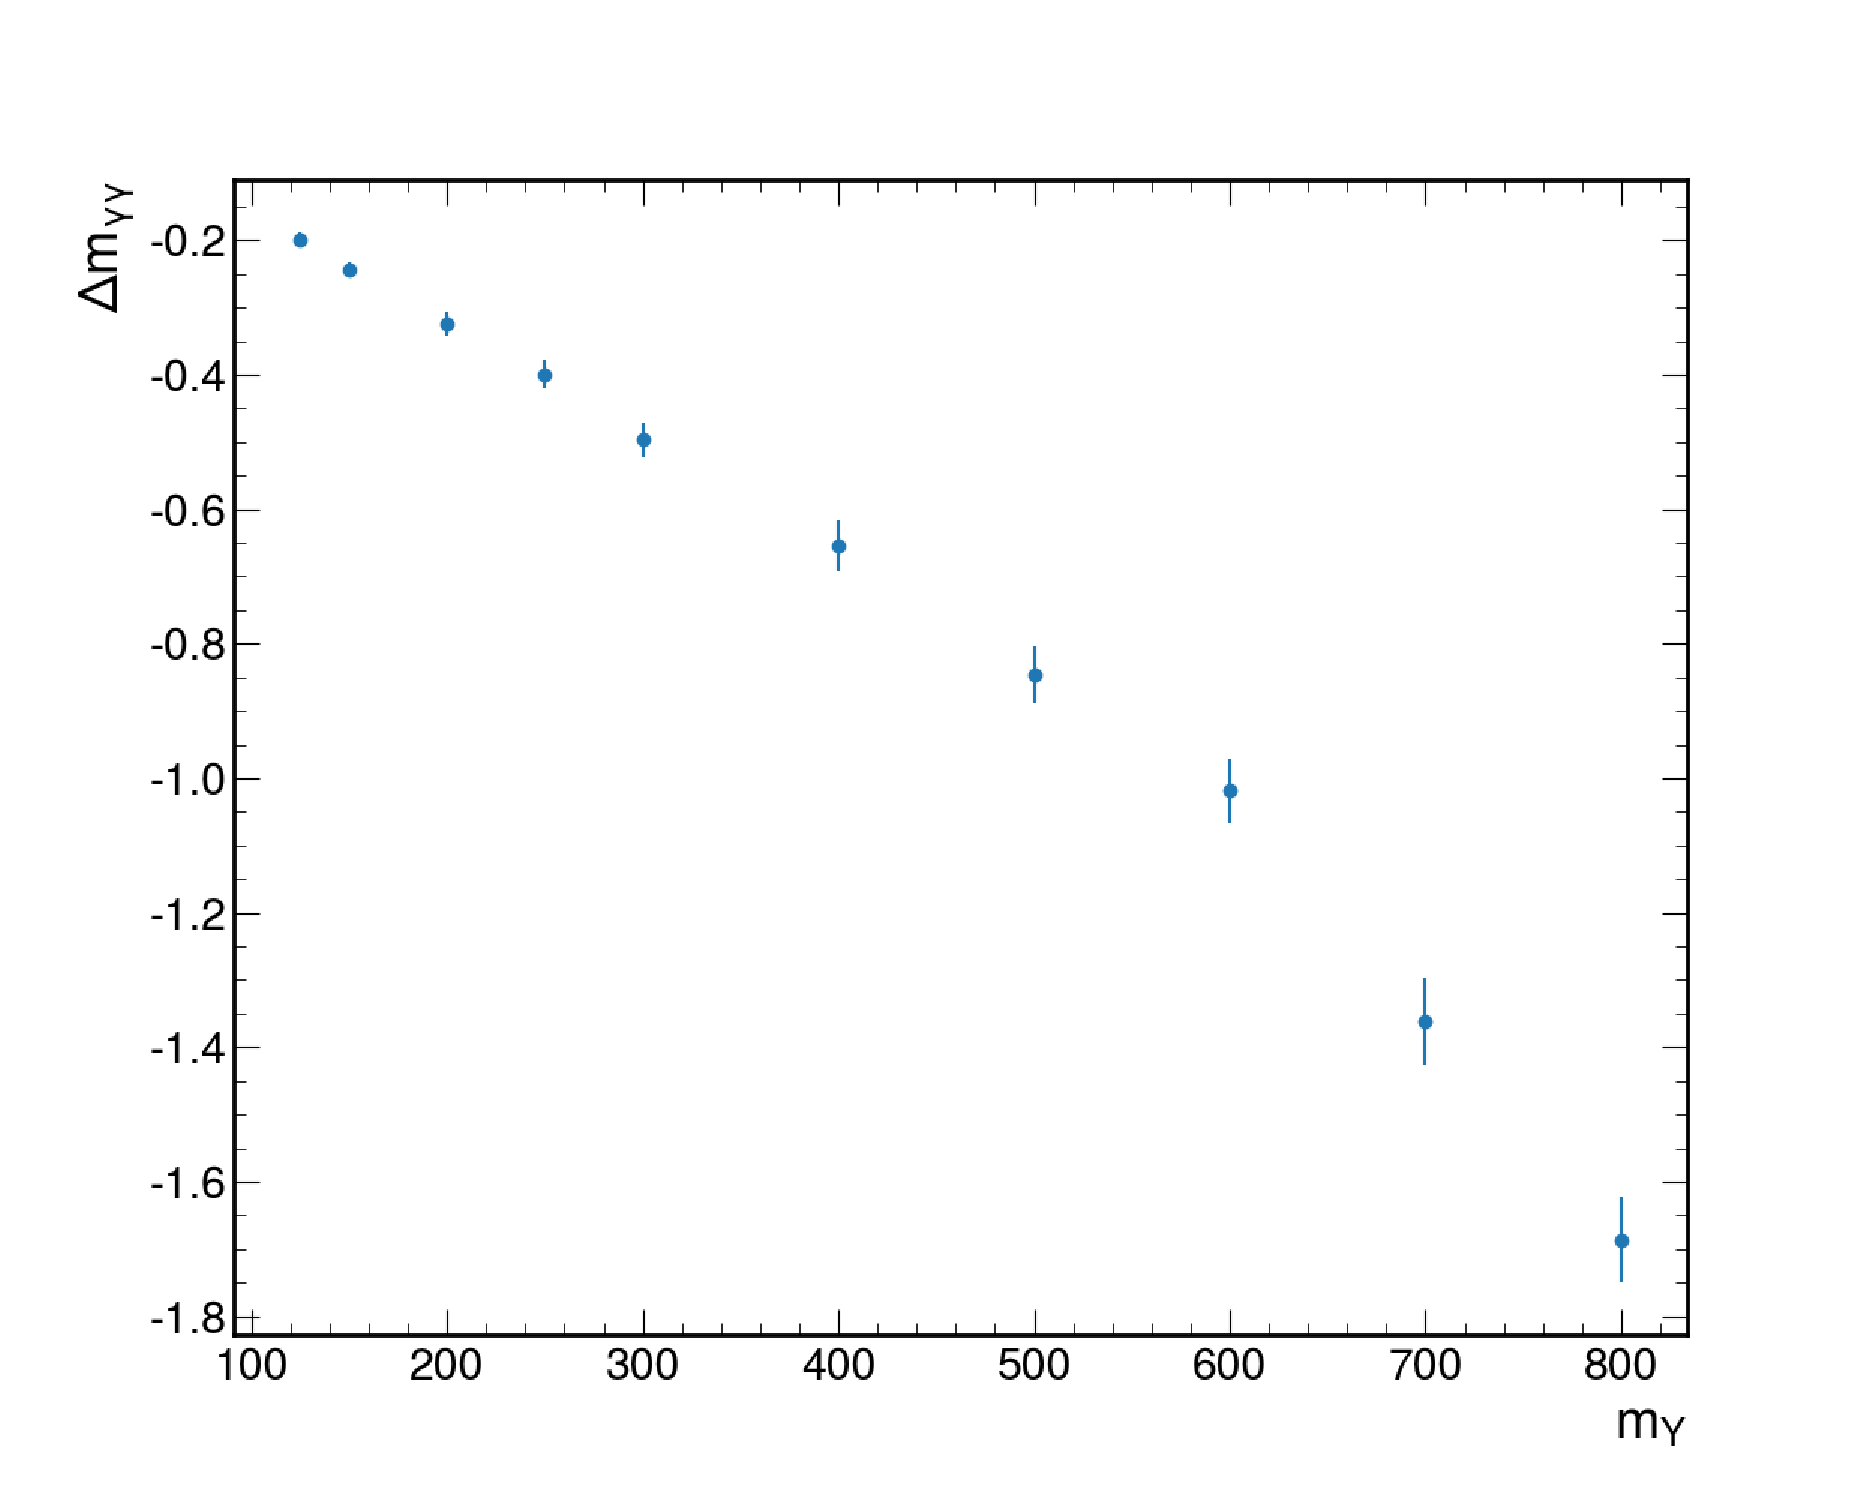
\includegraphics[width=0.49\textwidth]{Figures/Dihiggs/signal/shape_change/y_gg_high_mass_my_dm.pdf}
  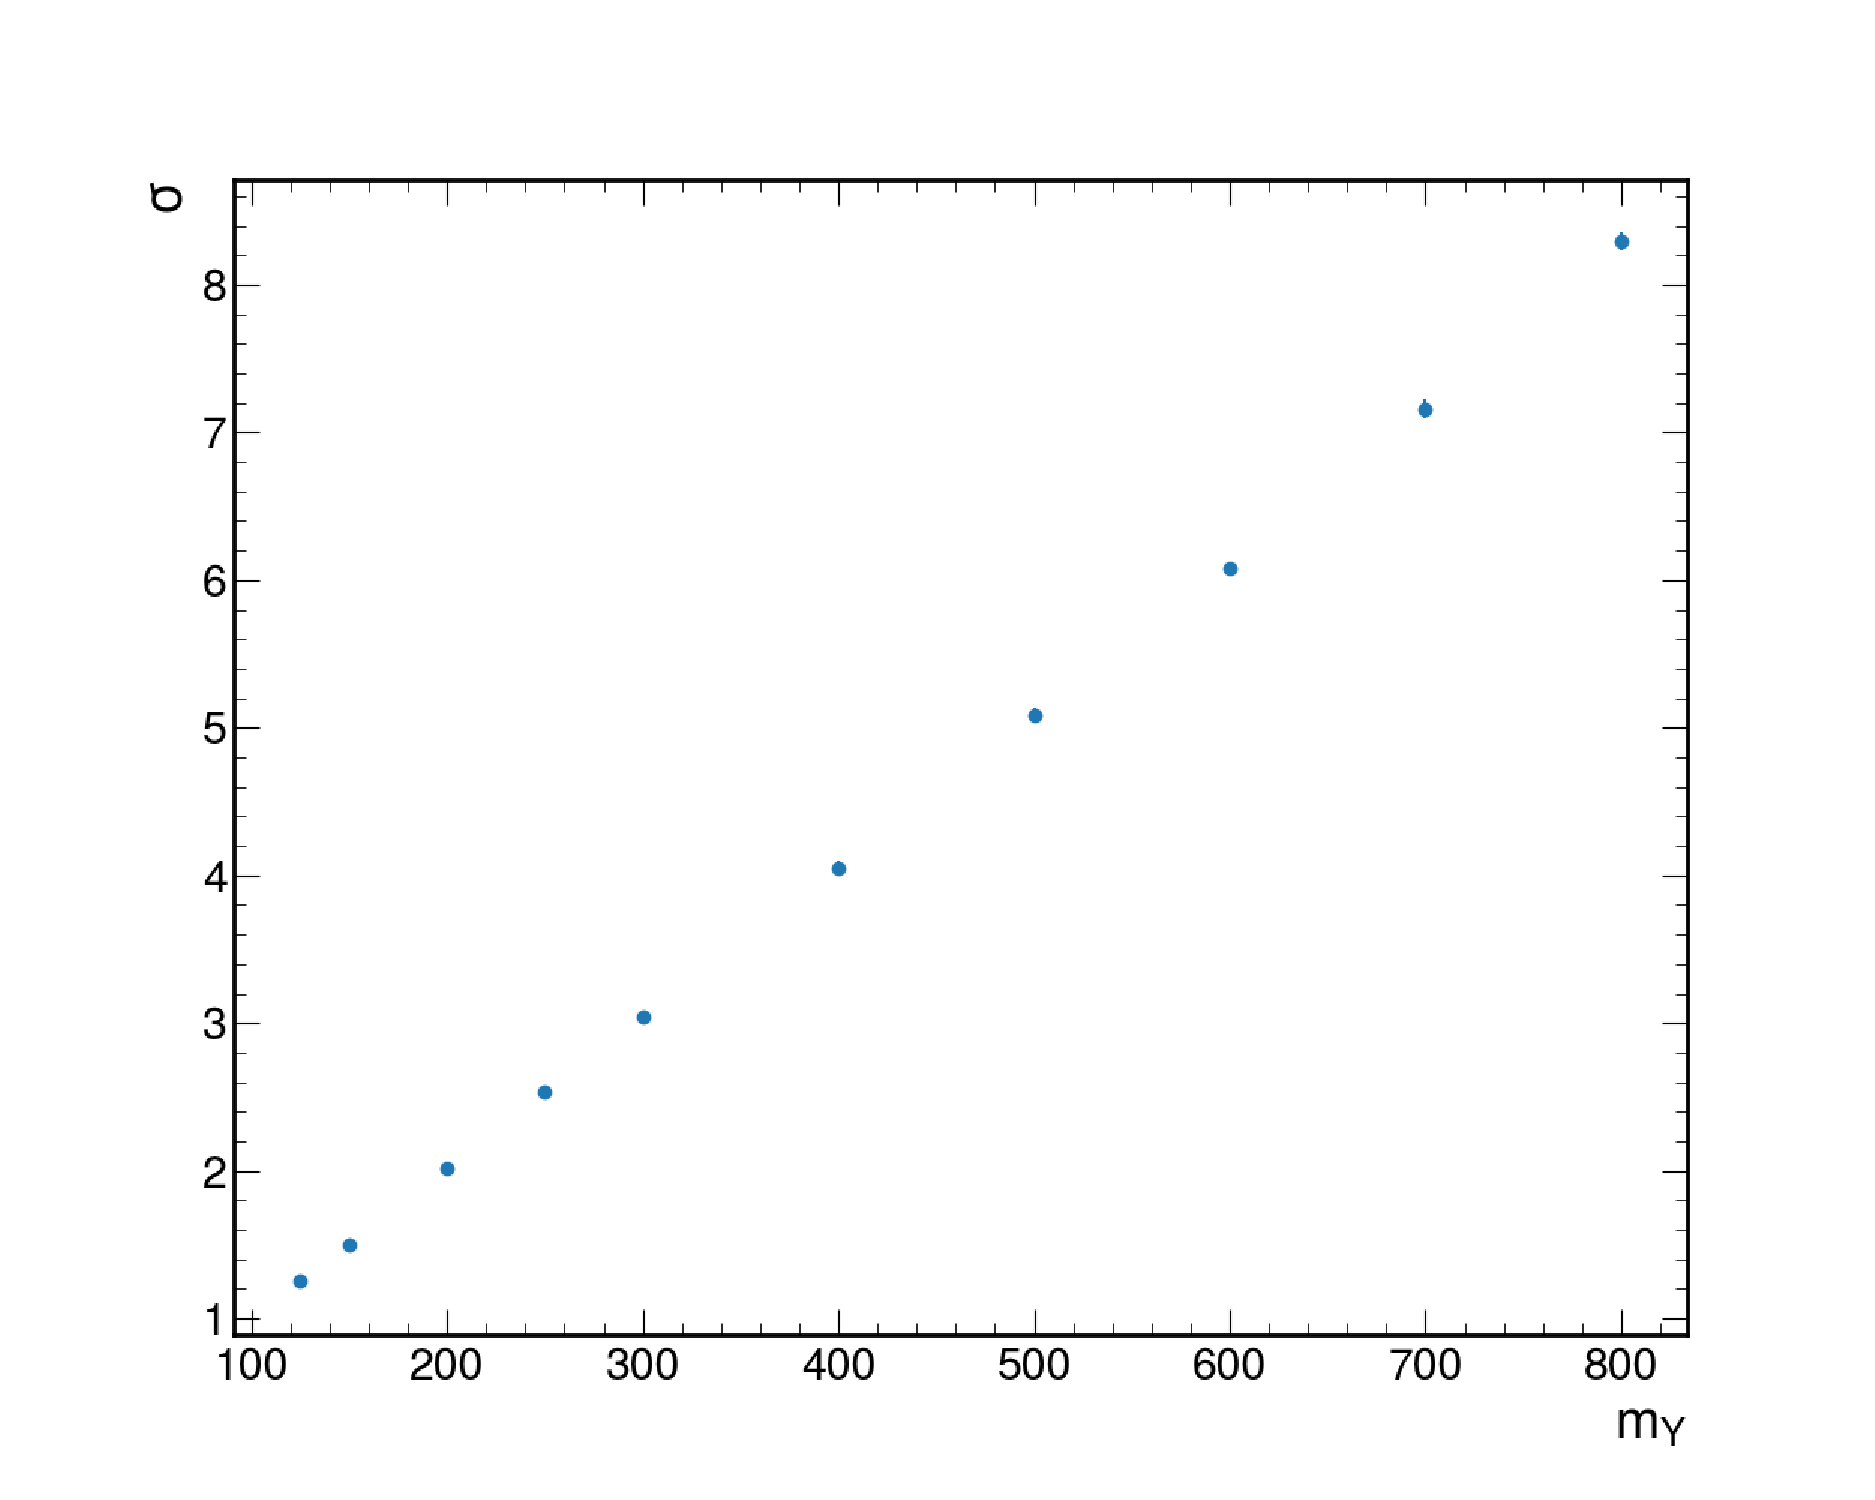
\includegraphics[width=0.49\textwidth]{Figures/Dihiggs/signal/shape_change/y_gg_high_mass_my_sigma.pdf} \\
  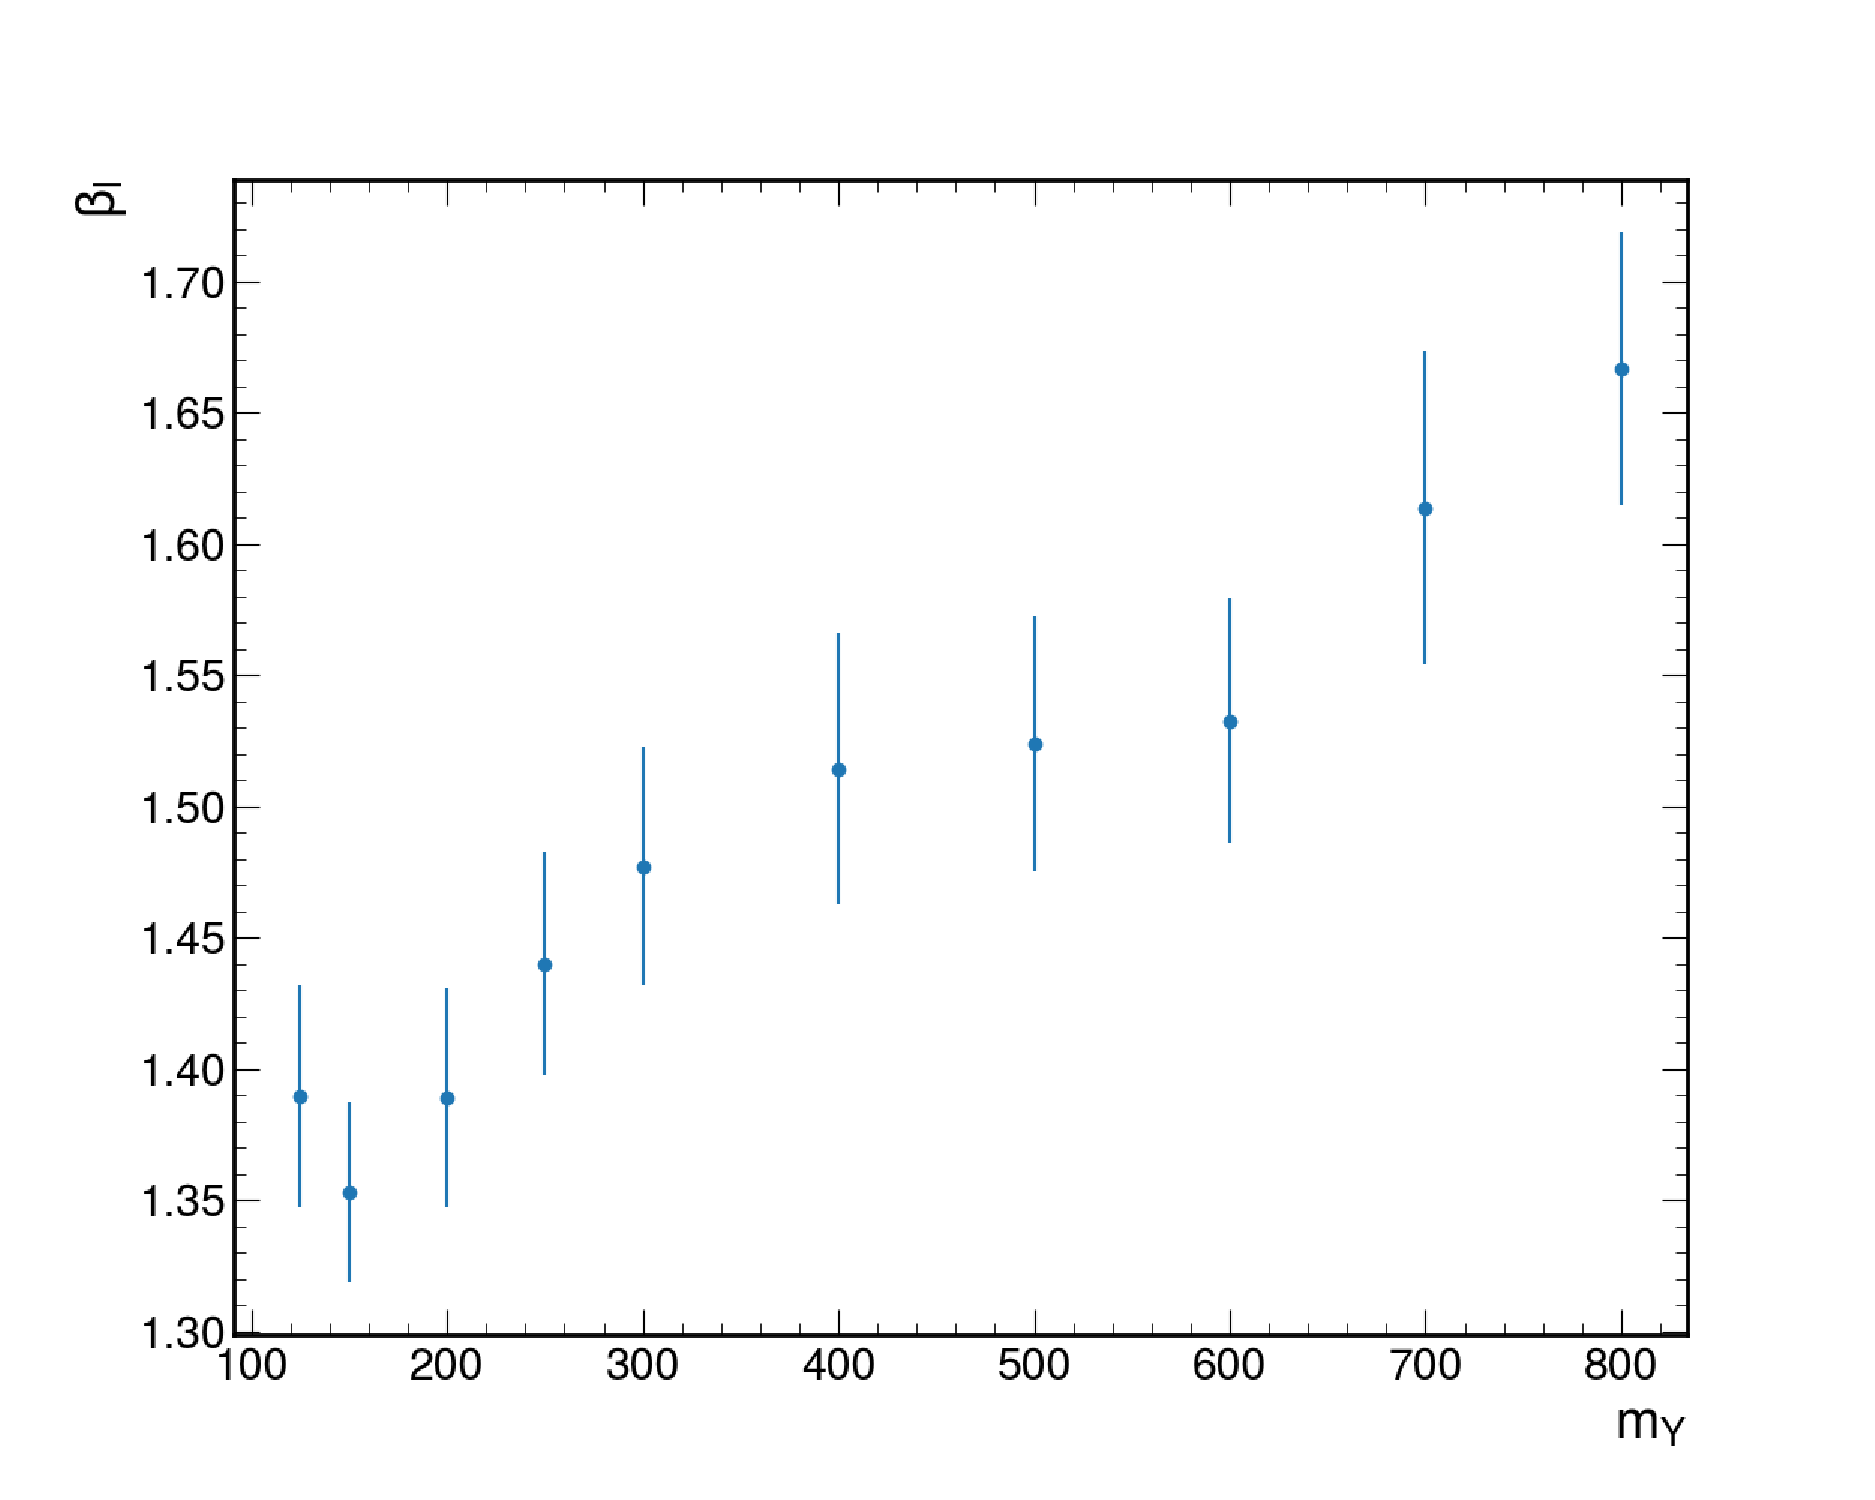
\includegraphics[width=0.49\textwidth]{Figures/Dihiggs/signal/shape_change/y_gg_high_mass_my_bl.pdf}
  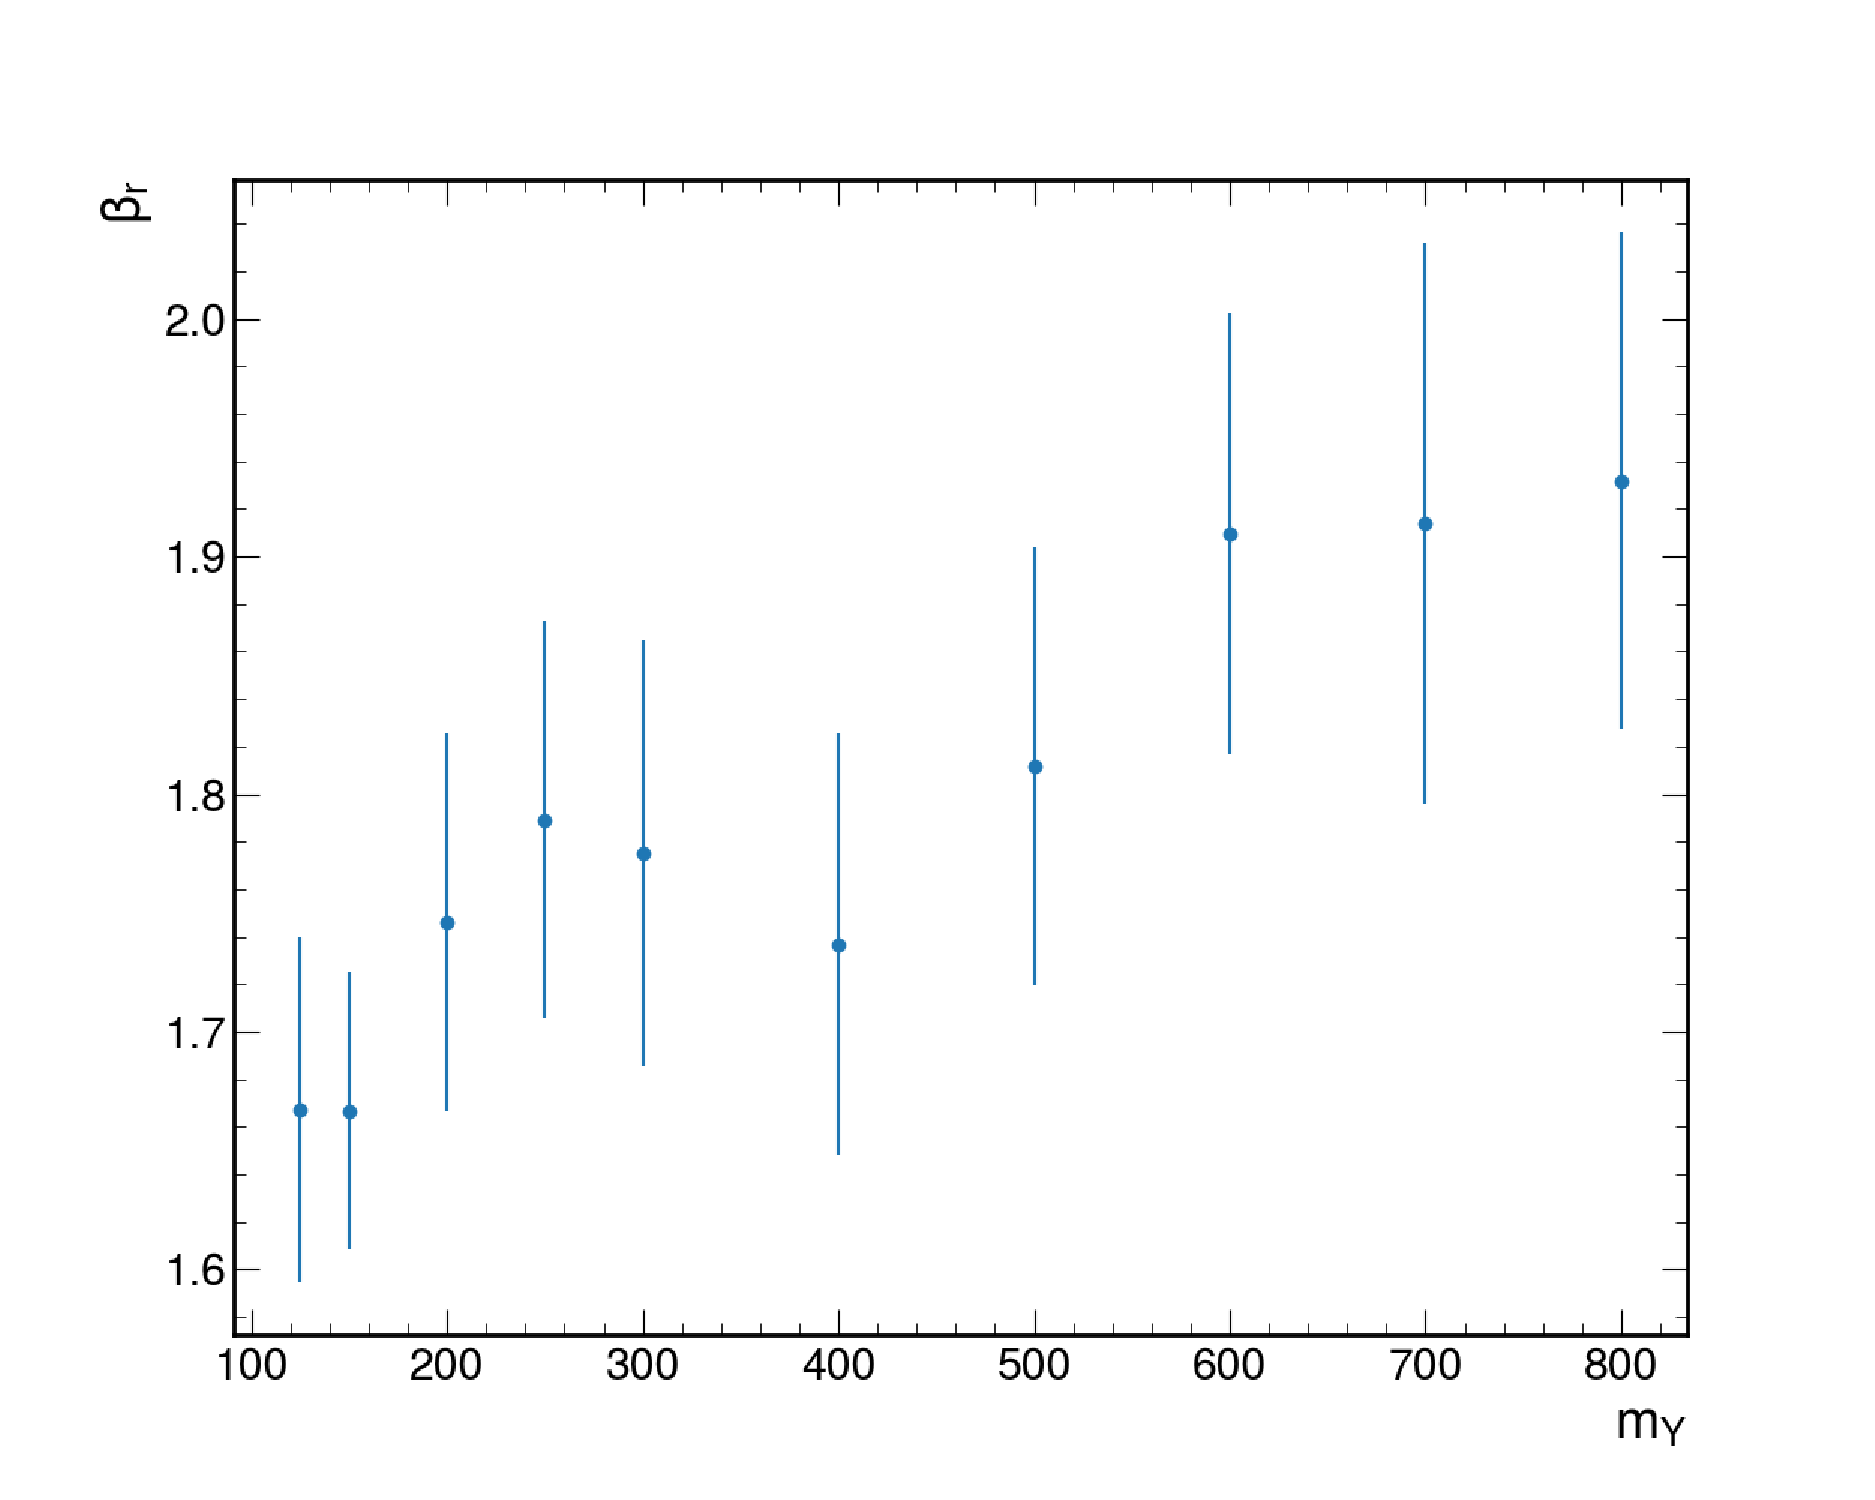
\includegraphics[width=0.49\textwidth]{Figures/Dihiggs/signal/shape_change/y_gg_high_mass_my_br.pdf} \\
  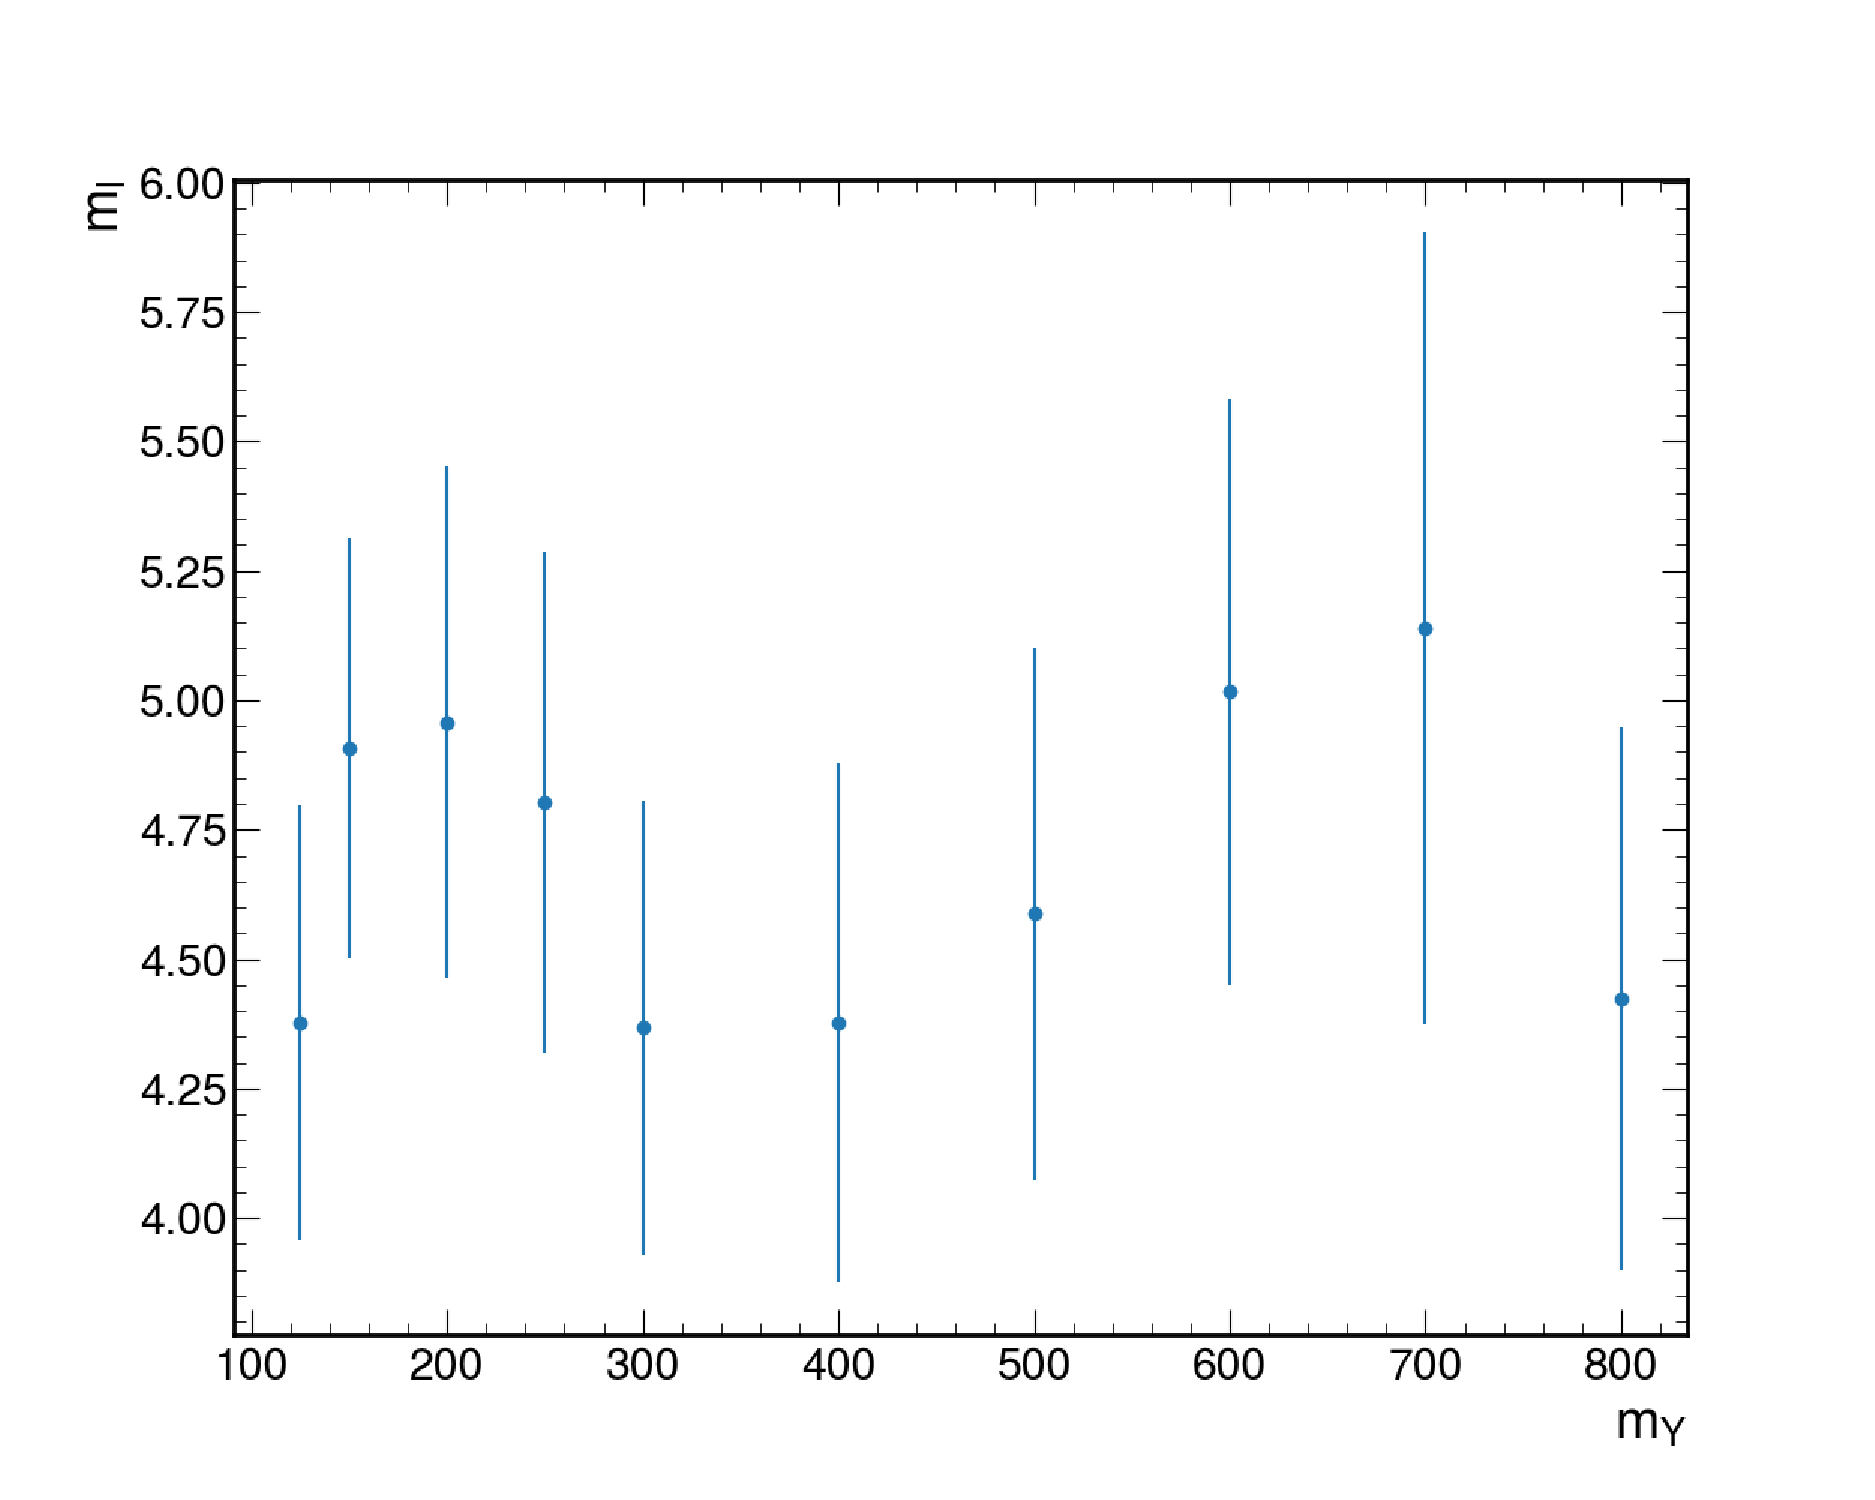
\includegraphics[width=0.49\textwidth]{Figures/Dihiggs/signal/shape_change/y_gg_high_mass_my_ml.pdf}
  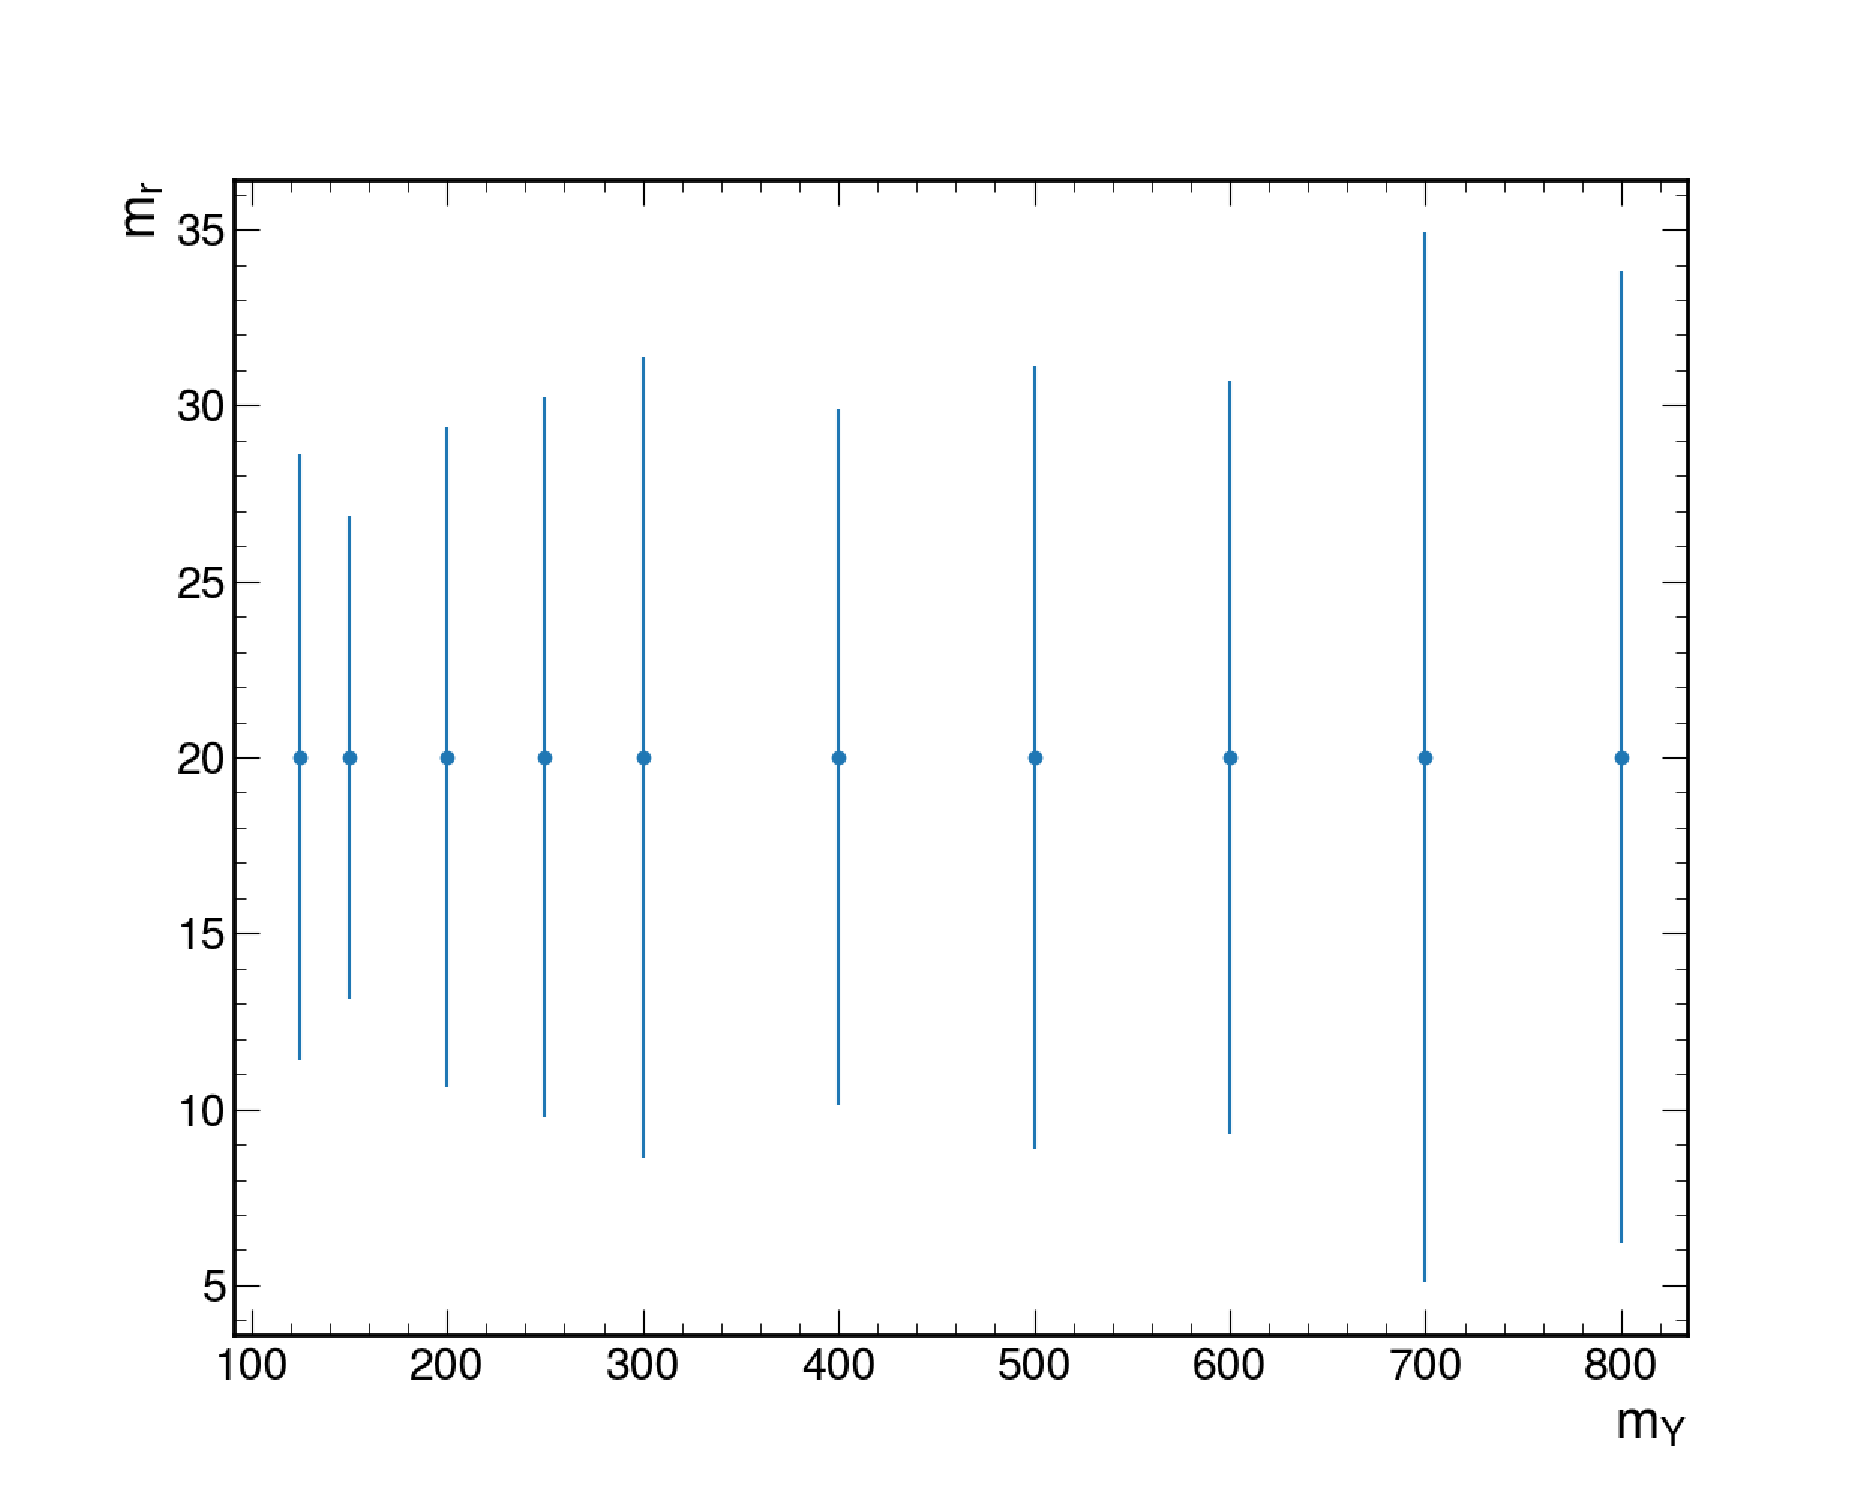
\includegraphics[width=0.49\textwidth]{Figures/Dihiggs/signal/shape_change/y_gg_high_mass_my_mr.pdf} 
  \caption[DCB Shape Parameters as a Function of \mY in the \XYH Searches]{Fitted shape parameters as a function of \mY for the \XYggHtt search where $\mY=1000$\GeV. These models are derived from MC across all years with a requirement on the pNN score of $\tilde{f}(\vec{x};m_X,m_Y)>0.99$ placed which is representative of the purest categories in the analysis.}\label{fig:shape_change_y_gg_high_mass_my}
\end{figure}

\subsection{Nonresonant Background}\label{sec:non_res_bkg_modelling}

The nonresonant background models are derived directly from data, where the sidebands regions, i.e.\ regions of \mgg well separated from the signal peak, are able to constrain the rate and shape of the background in the signal region. The methodology is outlined first for the \XHH and \XYttHgg searches and then the differences for the \XYggHtt searches are described. 

\subsubsection{\XHH and \XYttHgg Searches}

The distribution of \mgg in data and background MC after preselection for the \XHH and \XYttHgg searches is shown in \cref{fig:mgg_data_bkg_mc}. The nonresonant component of the background has a smoothly falling \mgg distribution. There is not a single, well-motivated analytical function to describe this distribution, so multiple \textit{families} of functions, listed in \cref{tab:bmodel_functions}, are considered. Within a family, there are functions of varying \textit{orders}, for example, for a sum of exponentials, the order corresponds to the number of exponentials in the sum. A higher order means more parameters in the function, and therefore greater freedom in the shape of the function. 

\begin{figure}
  \centering
  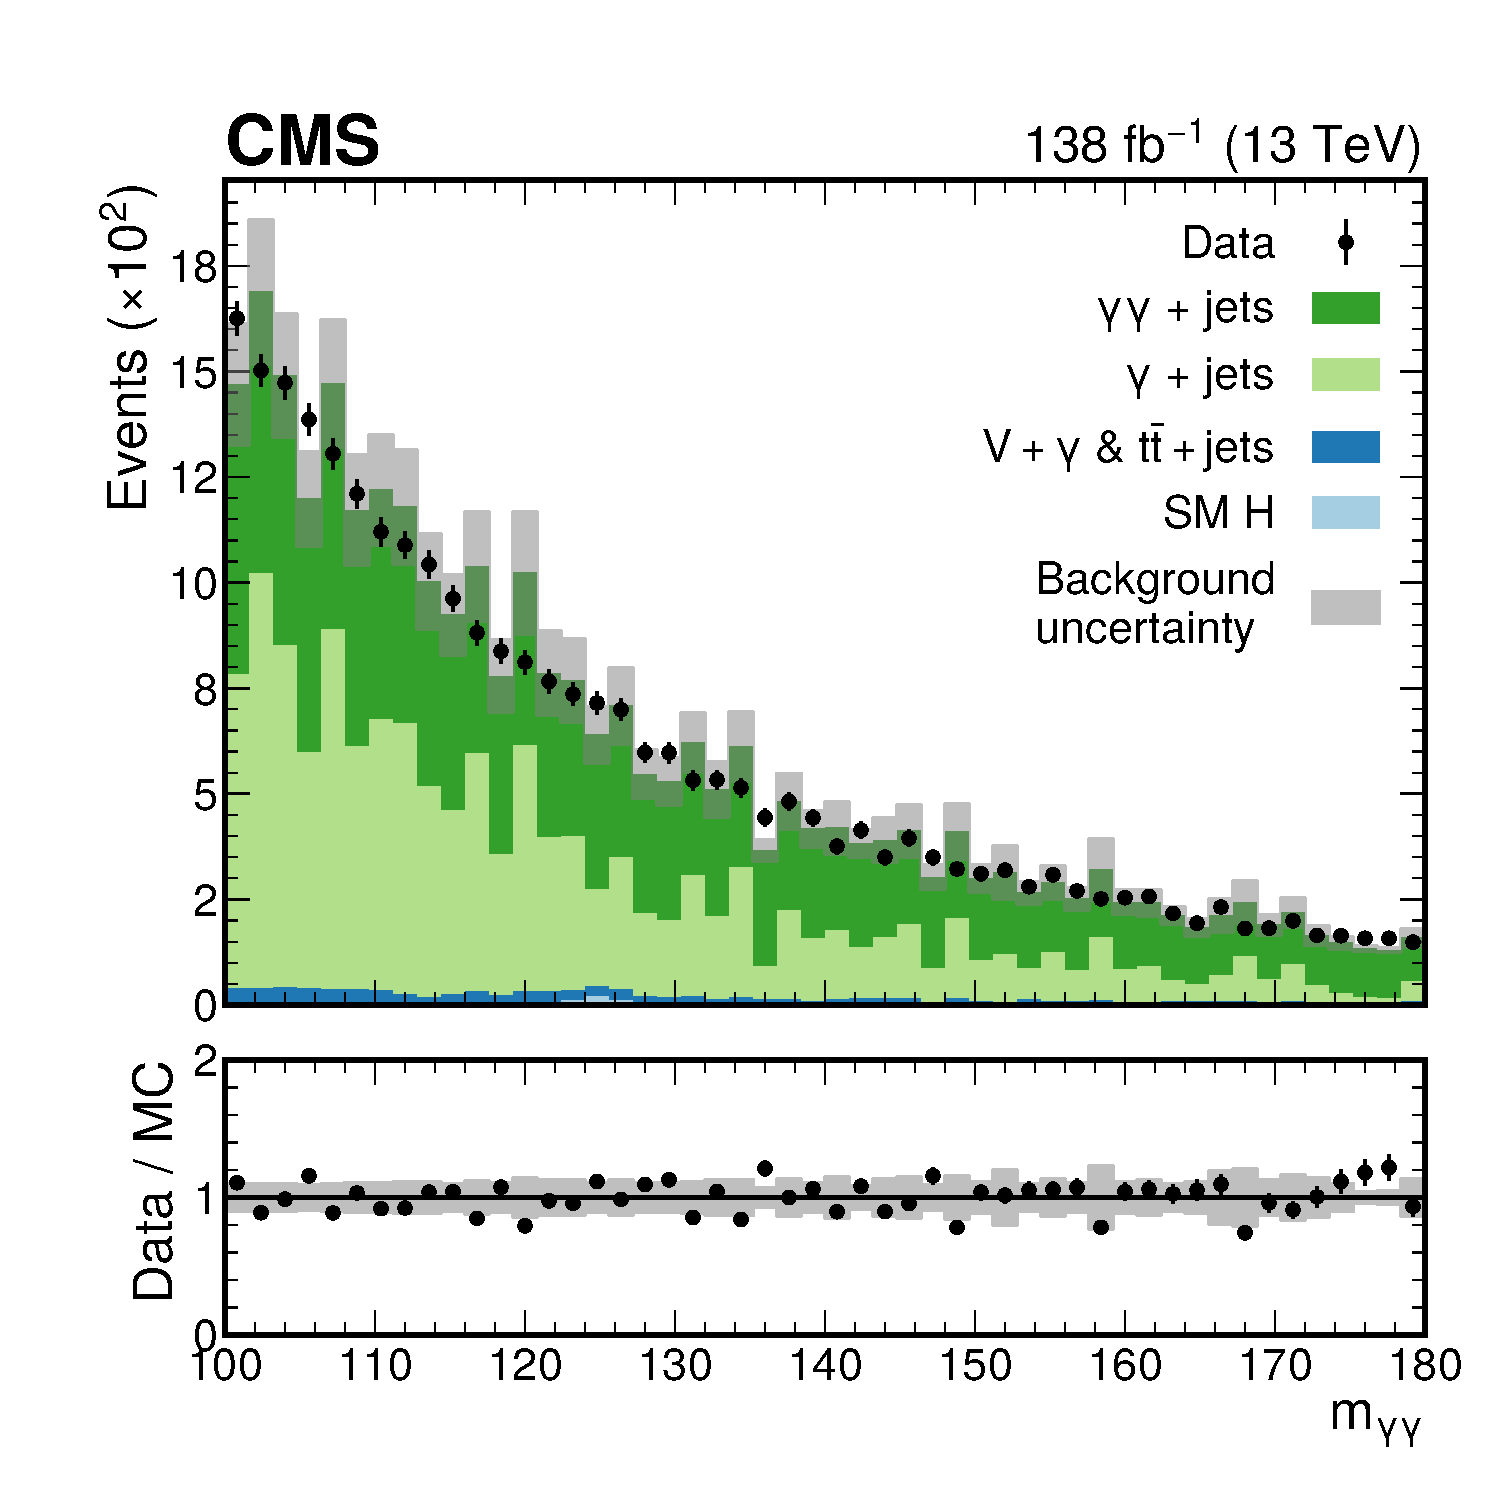
\includegraphics[width=0.6\textwidth]{Figures/Dihiggs/diphoton_mass.pdf}
  \caption[Distribution of \mgg in Data and Background MC After Preselection for the \XHH and \XYttHgg Searches]{Distribution of \mgg in data and background MC after preselection for the \XHH and \XYttHgg searches. The background MC is normalized to data and its statistical uncertainty is indicated by the grey shaded bands.}\label{fig:mgg_data_bkg_mc}
\end{figure}

\begin{table}
  \caption[Function Families Used to Model the Nonresonant Background in the \XHH and \XYttHgg Searches]{Function families considered for modelling the nonresonant background in the \XHH and \XYttHgg searches with the discrete profiling method. Each function is shown for order, $N$, and the free parameters of the functions are denoted $p_i$.}\label{tab:bmodel_functions}
  \centering
  \renewcommand{\arraystretch}{2}
  \begin{tabular}{cc}
    \toprule
    Name & Formula \\
    \midrule
    Sum of exponentials & $f_N(x) = \sum^N_{i=0} p_{2i} \exp(p_{2i+1}x)$ \\
    Sum of power laws & $f_N(x) = \sum^N_{i=0} p_{2i}x^{-p_{2i+1}}$ \\
    Bernstein polynomials & $f_N(x) = \sum^N_{i=0} p_i {N \choose i}x^i(1-x)^{N-i}$ \\
    Laurent series & $f_N(x) = \sum^N_{i=0} p_i x^{-4+g(i)}; \quad g(i) = \sum^i_{j=0} (-1)^j j$ \\
    Exponential of a polynomial & $ f_N(x) = \exp\left(\sum_{i=0}^N p_i x^i\right)$ \\
    \bottomrule
  \end{tabular}
\end{table}

If a function is chosen that does not accurately describe the underlying \mgg distribution, that choice could bias the final results. Therefore, an approach must be taken that introduces an uncertainty related to the choice of function. This is done by using the \textit{discrete profiling} method~\cite{Dauncey:2014xga}, where the choice of function is encoded as a discrete nuisance parameter which is profiled in the likelihood fit to data. This leads to an increased uncertainty on the parameter of interest that corresponds to the size of the impact that the discrete nuisance parameter has on the fit. 

Ideally, the discrete nuisance parameter could correspond to the choice between an infinite number of functions (beyond those listed in \cref{tab:bmodel_functions}) but this is practically impossible to achieve. Instead, a subset of functions, called an \textit{envelope}, is chosen that contains functions that fit well to the data, and have sufficiently different shapes such that a fit with the envelope is a good approximation of a fit with infinitely many functions.

Every analysis category has its own envelope of functions. The building of a category's envelope begins by performing a maximum likelihood fit with the lowest-order function of each family in \cref{tab:bmodel_functions} to the \mgg distribution in data in the analysis category. Only the sidebands of the \mgg distribution are used, which excludes the $115 < \mgg < 135$\GeV region, so that a signal peak at about 125\GeV will not influence the fit.  This procedure continues up to an order corresponding to 6 free parameters, or until an order is reached where a loose goodness-of-fit criteria, $p\text{-value}>0.01$, is satisfied, in which case the function is added to the envelope.

Starting from the functions that satisfy the loose goodness-of-fit criteria, further orders are added according to an F-test requirement~\cite{10.2307/2340521}. When adding a function of a higher order, the difference in $-2\ln\mathcal{L}$ between the two fits, $\Delta$, is used to calculate a p-value defined as:
\begin{equation}
  p = \int_\Delta^\infty \chi^2(x, m)\,dx
\end{equation}
where $\chi^2(x,m)$ is a $\chi^2$ distribution with $m$ degrees of freedom, and $m$ is the difference in the number of free parameters between the two orders. If the p-value is less than 0.05, the fit quality is deemed to have improved sufficiently enough, and the function is added to the envelope. If it is more than 0.05, the function is not added, and no more functions of that family are considered. This continues until a maximum order corresponding to 6 free parameters is reached.

The pdf of the nonresonant background in an analysis category is then given by:
\begin{equation}
  f(\mgg;\vec{\Psi}_1,\vec{\Psi}_2\cdots\vec{\Psi}_n,\nu) = \begin{cases}
    f_1(\mgg;\vec{\Psi}_1) & \text{if } \nu=1 \\
    f_2(\mgg;\vec{\Psi}_2) & \text{if } \nu=2 \\
    \vdots & \vdots \\
    f_n(\mgg;\vec{\Psi}_n) & \text{if } \nu=n 
  \end{cases} 
\end{equation}
where $\nu$ is the discrete nuisance parameter, and $f_i$ is the $i$th function of the envelope of $n$ functions. The expected number of nonresonant background events in an analysis category is left as a free parameter that is fit in data.

Examples of the envelope construction from the $(\mX,\mY)=(300,50)$\GeV mass point in the \XYttHgg search, are shown in \cref{fig:envelope_examples_ytt} for categories with 10, 20, 80 and 320 expected background events. In general, the envelopes contain a single function from each family, and do not contain functions with orders greater than 2. This is a consequence of the small number of expected background events in the analysis categories. To illustrate this point, an envelope is constructed for a category with the remaining events that pass preselection but not the pNN selection, and is also shown in \cref{fig:envelope_examples_ytt}. There, functions of up to order 4 are included. 

\begin{figure}
  \centering
  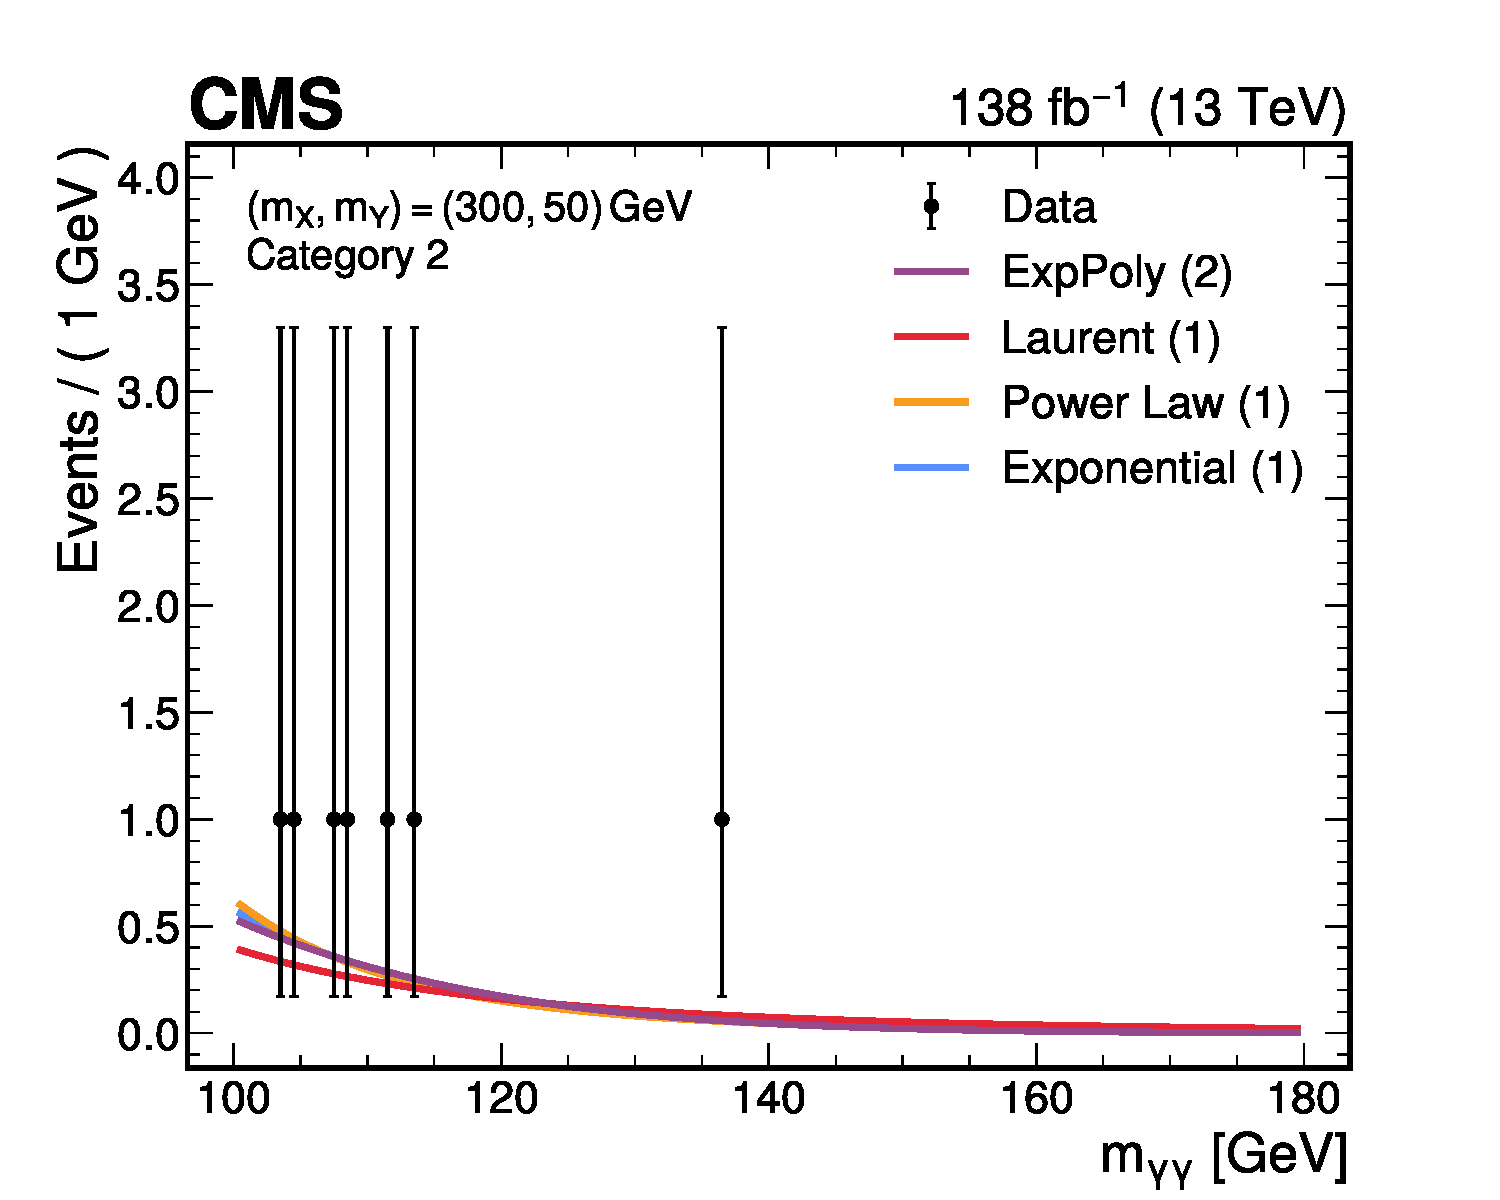
\includegraphics[width=.49\linewidth]{Figures/Dihiggs/background/envelope/y_tautau/bkgmodel_pdfs_ggttresmx300my50cat2.pdf}
  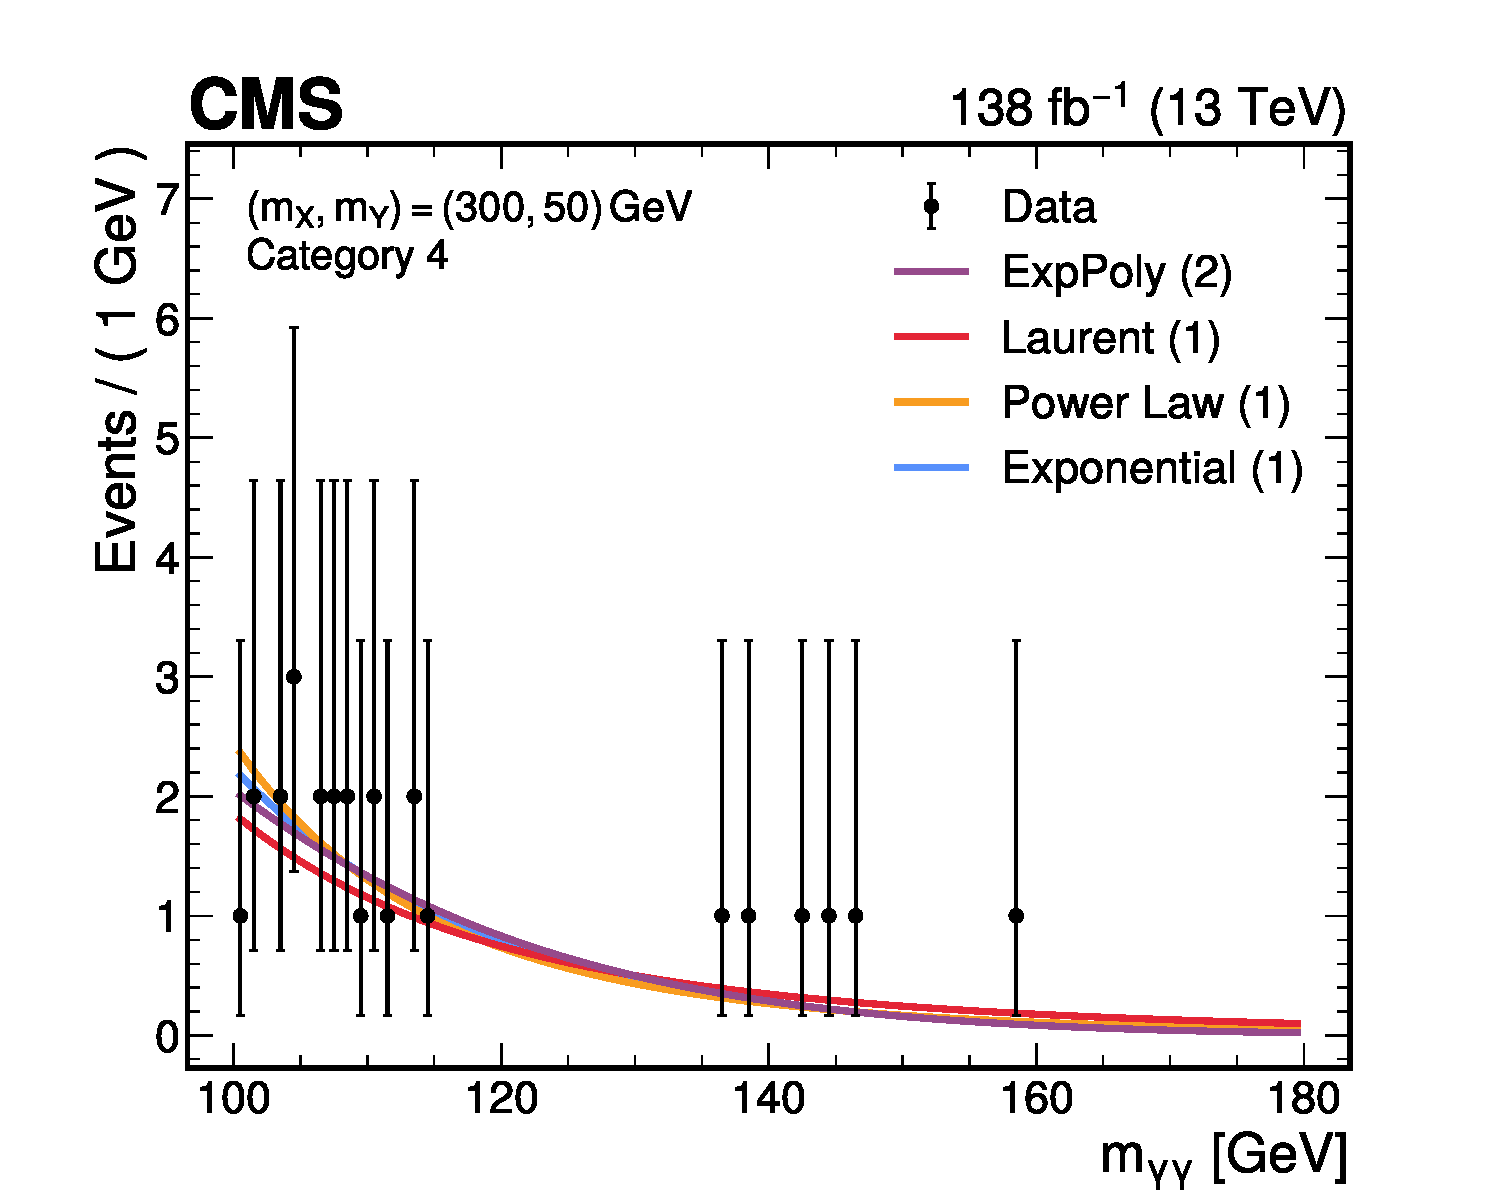
\includegraphics[width=.49\linewidth]{Figures/Dihiggs/background/envelope/y_tautau/bkgmodel_pdfs_ggttresmx300my50cat4.pdf}
  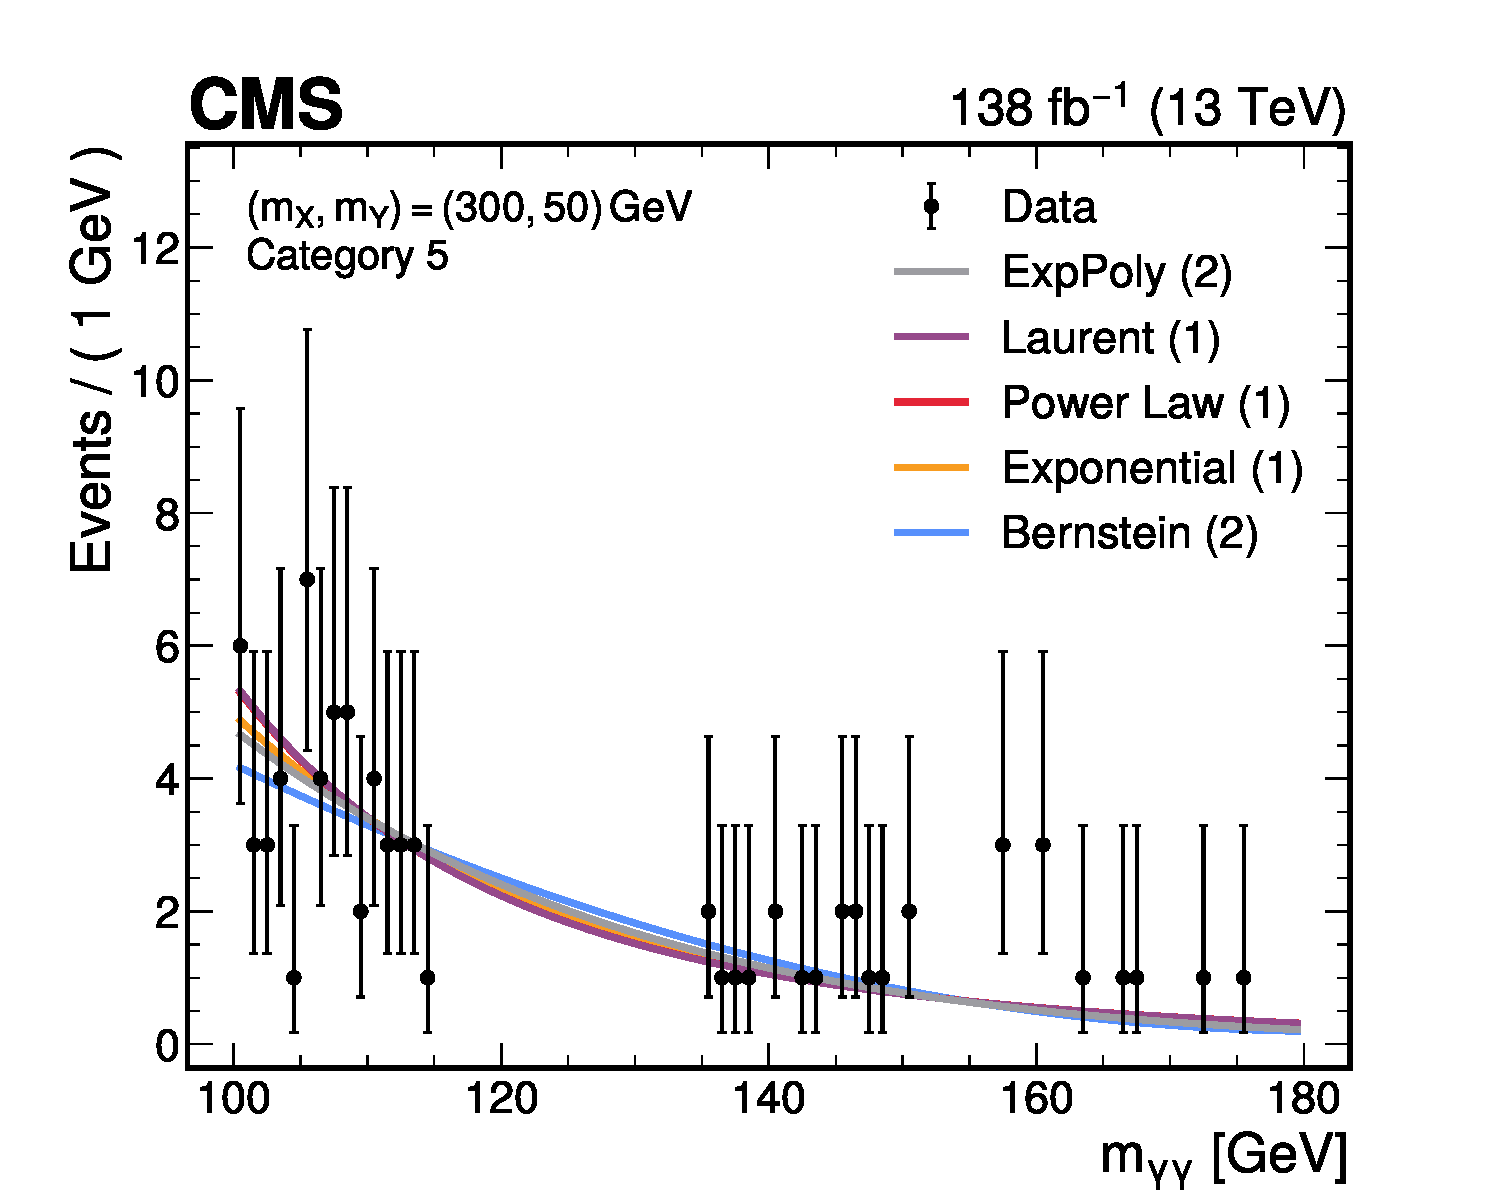
\includegraphics[width=.49\linewidth]{Figures/Dihiggs/background/envelope/y_tautau/bkgmodel_pdfs_ggttresmx300my50cat5.pdf}
  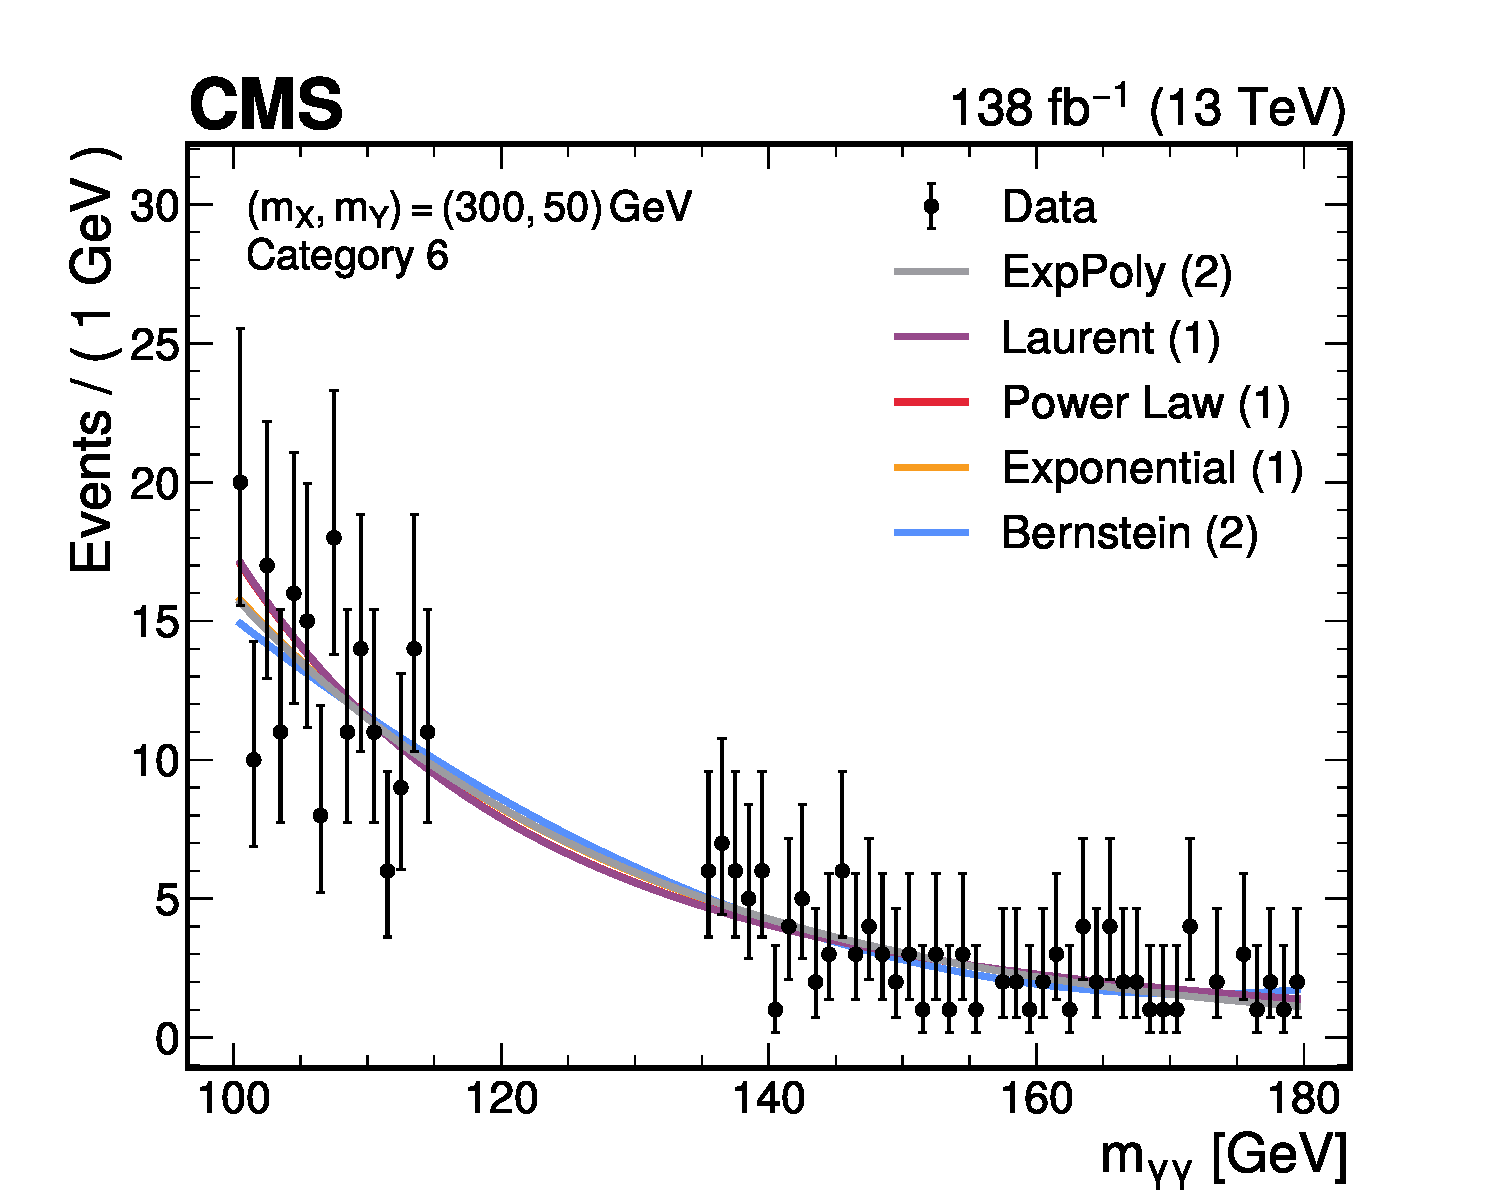
\includegraphics[width=.49\linewidth]{Figures/Dihiggs/background/envelope/y_tautau/bkgmodel_pdfs_ggttresmx300my50cat6.pdf}
  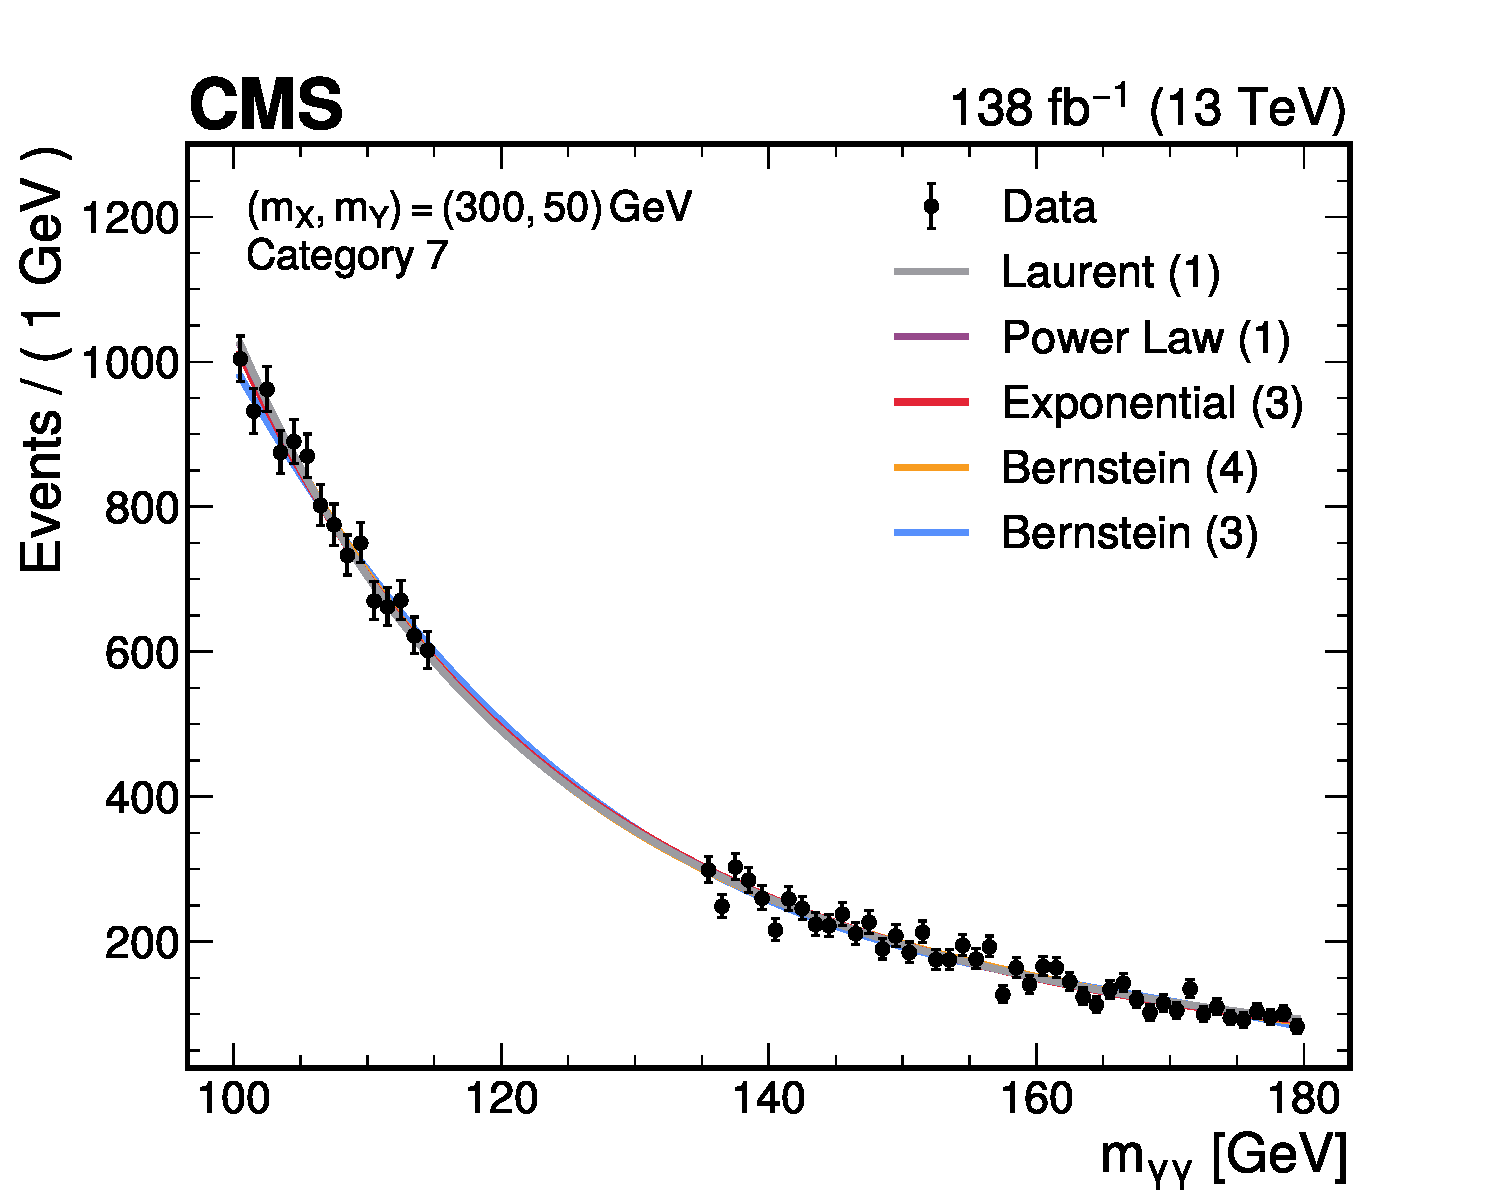
\includegraphics[width=.49\linewidth]{Figures/Dihiggs/background/envelope/y_tautau/bkgmodel_pdfs_ggttresmx300my50cat7.pdf}
  \caption[Envelope Construction for $(\mX,\mY)=(300,50)$\GeV in the \XYttHgg Search]{Envelope construction for the $(\mX,\mY)=(300,50)$\GeV mass point in the \XYttHgg search. Shown are the \mgg distributions in data in the sideband regions for categories 2, 4, 5 and 6 (top-left to middle-right) which are expected to have 10, 20, 80 and 320 background events respectively. An additional category (bottom) consisting of the events passing preselection but not passing the pNN selection, is also shown to illustrate how the envelope construction works in categories with more events. The functions entering the envelope are indicated in the legend and their fits to the \mgg distributions are shown in the plots.}\label{fig:envelope_examples_ytt}
\end{figure}

\subsubsection{\XYggHtt Searches}

The nonresonant background modelling in the \XYggHtt searches is done in a similar way to the \XHH and \XYttHgg searches, but with some differences. Firstly, the sidebands definition is changed to exclude a region of $\mY \pm (125\GeV/\mY)$, except for $\mY < 72$\GeV where the $\mgg < 68$\GeV region is kept so that there are enough events to perform the envelope construction. Only 4\% of the events from a $\mY=70$\GeV signal fall into this region so the impact from a potential signal in data on the envelope construction is likely to be small. For the low-mass search, the sideband definition is the only difference, and the final envelopes are not substantially different from those in the \XHH and \XYttHgg searches, as illustrated by examples for $(\mX,\mY)=(300,70)$\GeV in \cref{fig:envelope_examples_ygg_low}.

\begin{figure}
  \centering
  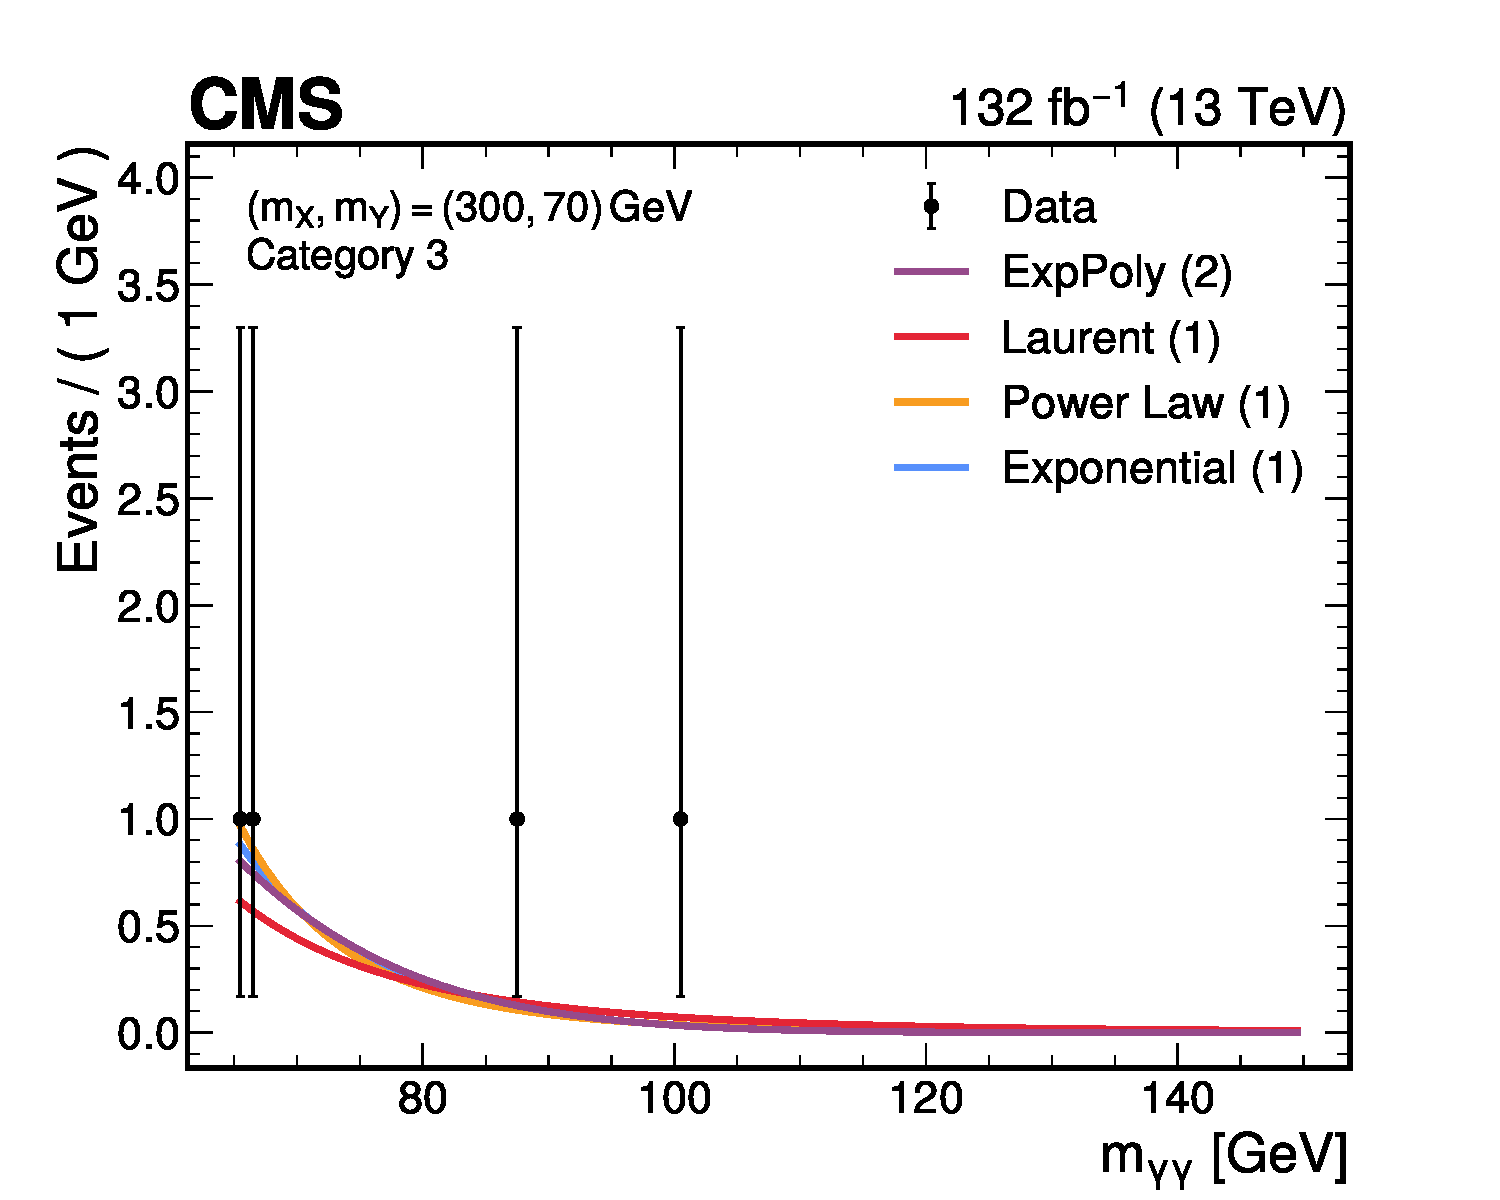
\includegraphics[width=.49\linewidth]{Figures/Dihiggs/background/envelope/y_gg_low_mass/bkgmodel_pdfs_ggttresmx300my70cat3.pdf}
  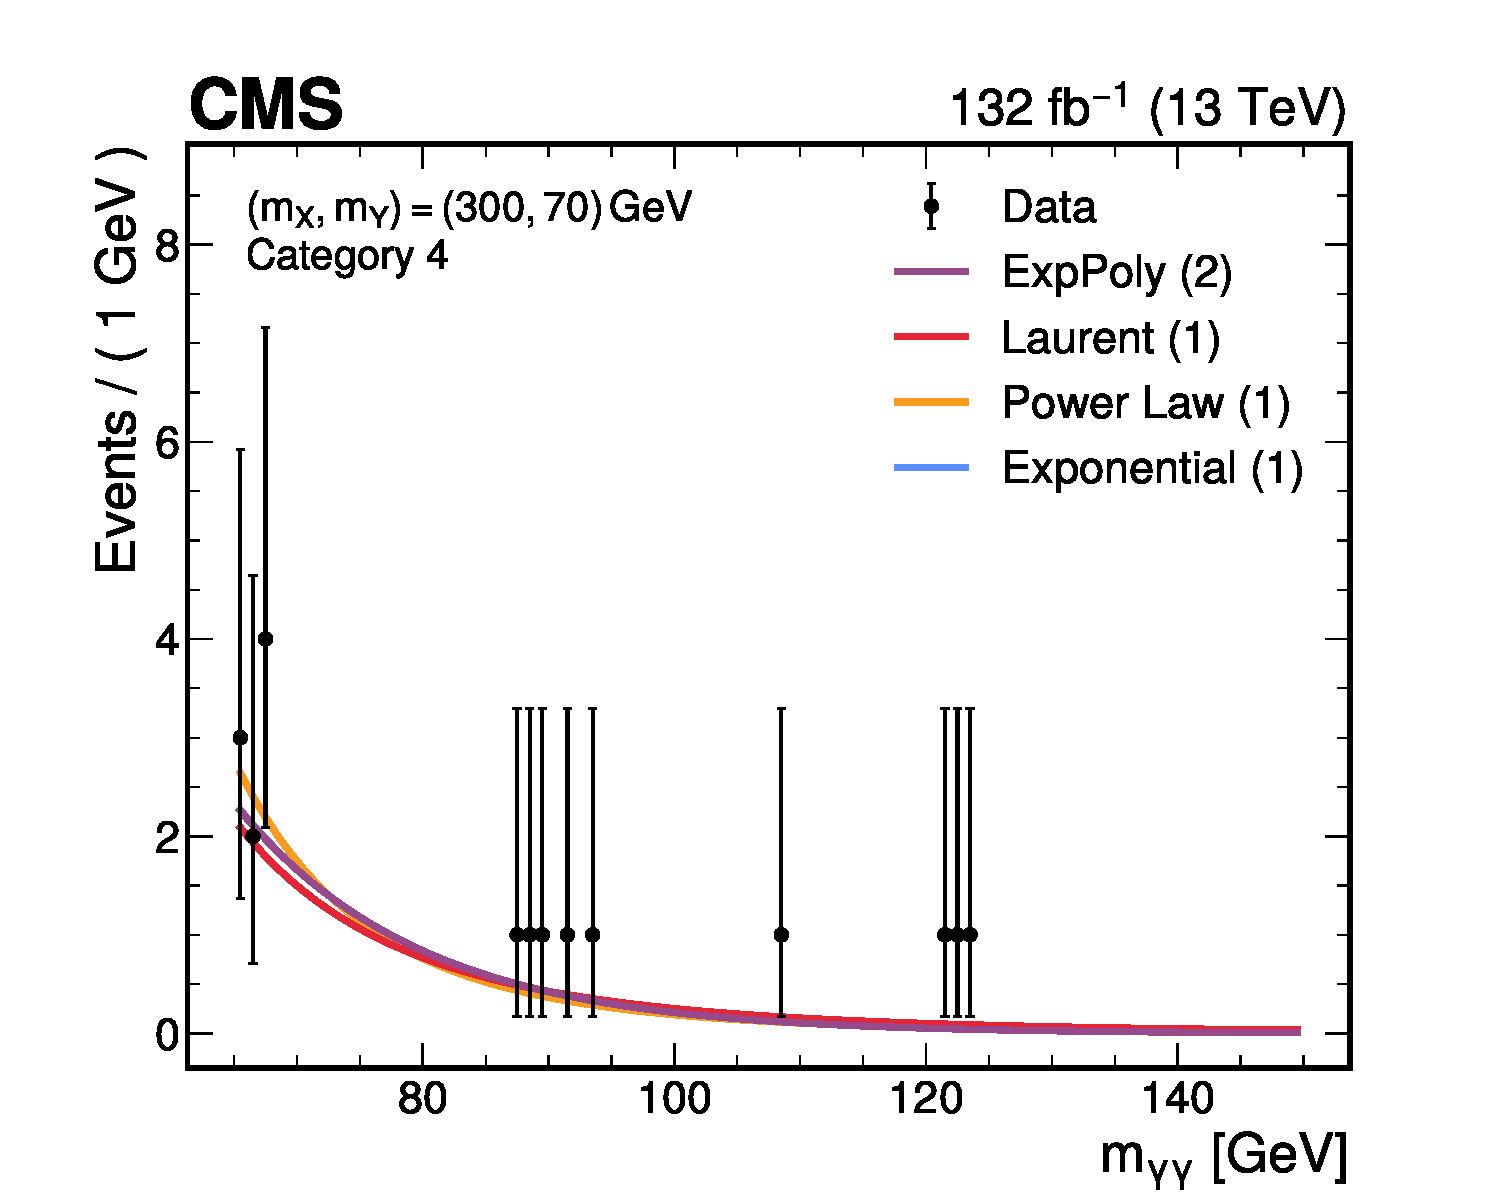
\includegraphics[width=.49\linewidth]{Figures/Dihiggs/background/envelope/y_gg_low_mass/bkgmodel_pdfs_ggttresmx300my70cat4.pdf}
  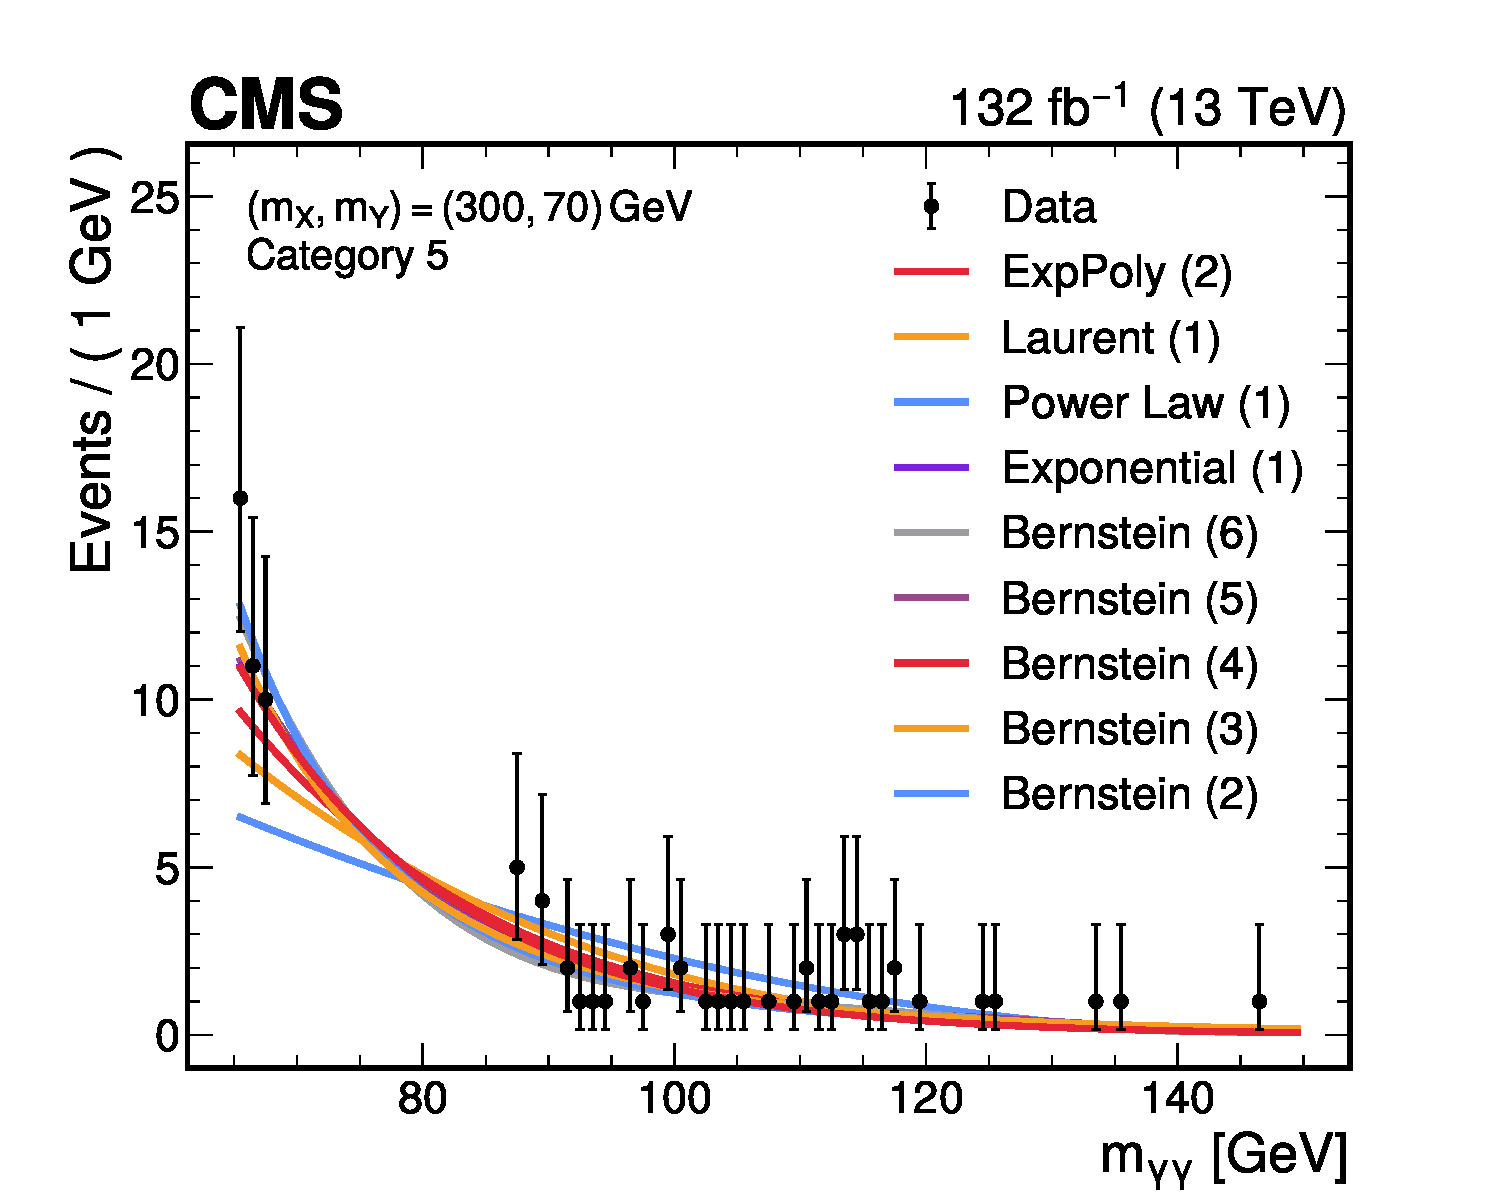
\includegraphics[width=.49\linewidth]{Figures/Dihiggs/background/envelope/y_gg_low_mass/bkgmodel_pdfs_ggttresmx300my70cat5.pdf}
  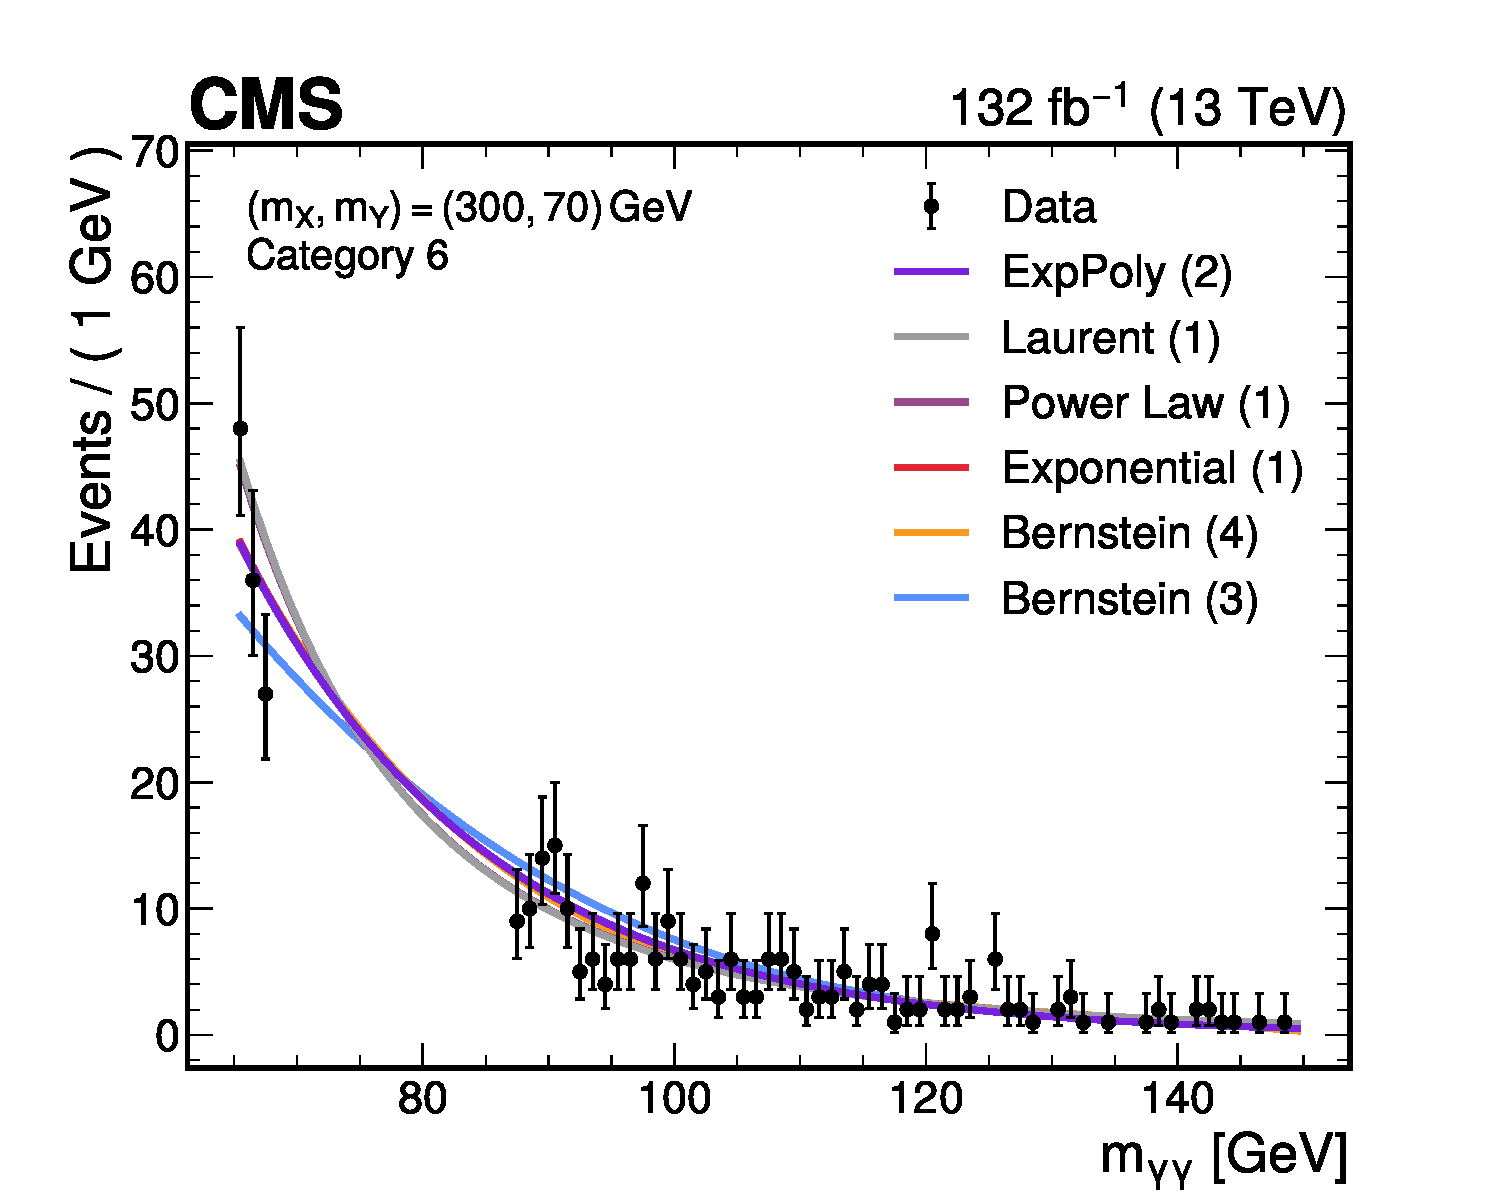
\includegraphics[width=.49\linewidth]{Figures/Dihiggs/background/envelope/y_gg_low_mass/bkgmodel_pdfs_ggttresmx300my70cat6.pdf}
  \caption[Envelope Construction for $(\mX,\mY)=(300,70)$\GeV in the Low-Mass \XYggHtt Search]{Envelope construction for the $(\mX,\mY)=(300,70)$\GeV mass point in the \XYggHtt search. Shown are the \mgg distributions in data in the sideband regions for categories 3, 4, 5 and 6 (top-left to middle-right) which are expected to have 10, 20, 80 and 320 background events respectively. The functions entering the envelope are indicated in the legend and their fits to the \mgg distributions are shown in the plots.}\label{fig:envelope_examples_ygg_low}
\end{figure}

In the high-mass \XYggHtt search, a further change is made to the function families considered. Over the larger \mgg range (up to 1\TeV), the Bernstein polynomials do not pass the loose goodness-of-fit criteria, so they were removed from consideration. To reintroduce some shape flexibility to the envelope, a new family of functions, referred to as Dijet functions, is added. The Dijet function is defined as:
\begin{equation}
  f_n(x) =
  \begin{cases}
      x^{-p_1}, & n = 1 \\
      (1 - x)^{p_1} x^{-p_2}, & n = 2 \\
      (1 - x)^{p_1} x^{- (p_2 + p_3 \ln x)}, & n = 3 \\
      (1 - x)^{p_1} x^{- (p_2 + p_3 \ln x + p_4 \ln^2 x)}, & n = 4 \\
      (1 - x)^{p_1} x^{- (p_2 + p_3 \ln x + p_4 \ln^2 x + p_5 \ln^3 x)}, & n = 5
  \end{cases}
\end{equation}
The suitability of this function family is demonstrated in \cref{fig:envelope_examples_ygg_high_cat7} for the category comprised of the remaining events after the pNN selection for the $(\mX,\mY) = (1000,700)$\GeV mass point where Dijet functions of up to order 3 are included in the envelope. 

\begin{figure}
  \centering
  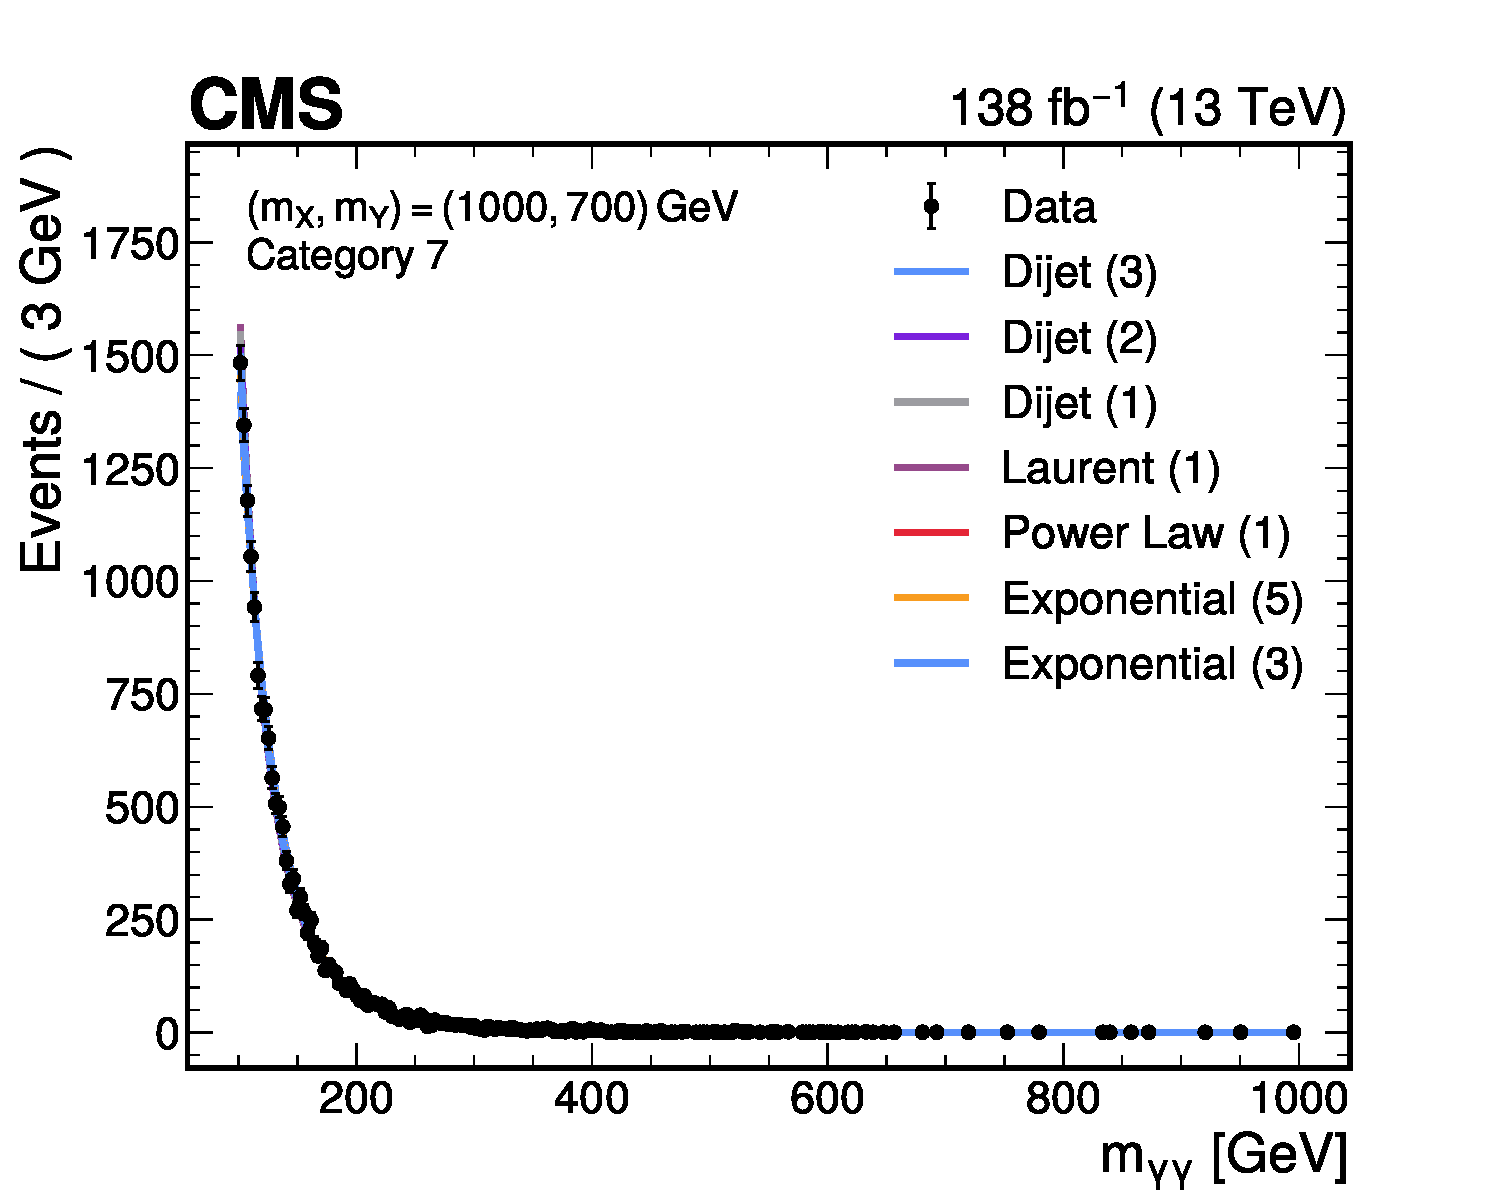
\includegraphics[width=.49\linewidth]{Figures/Dihiggs/background/envelope/y_gg_high_mass/bkgmodel_pdfs_ggttresmx1000my700cat7.pdf}
  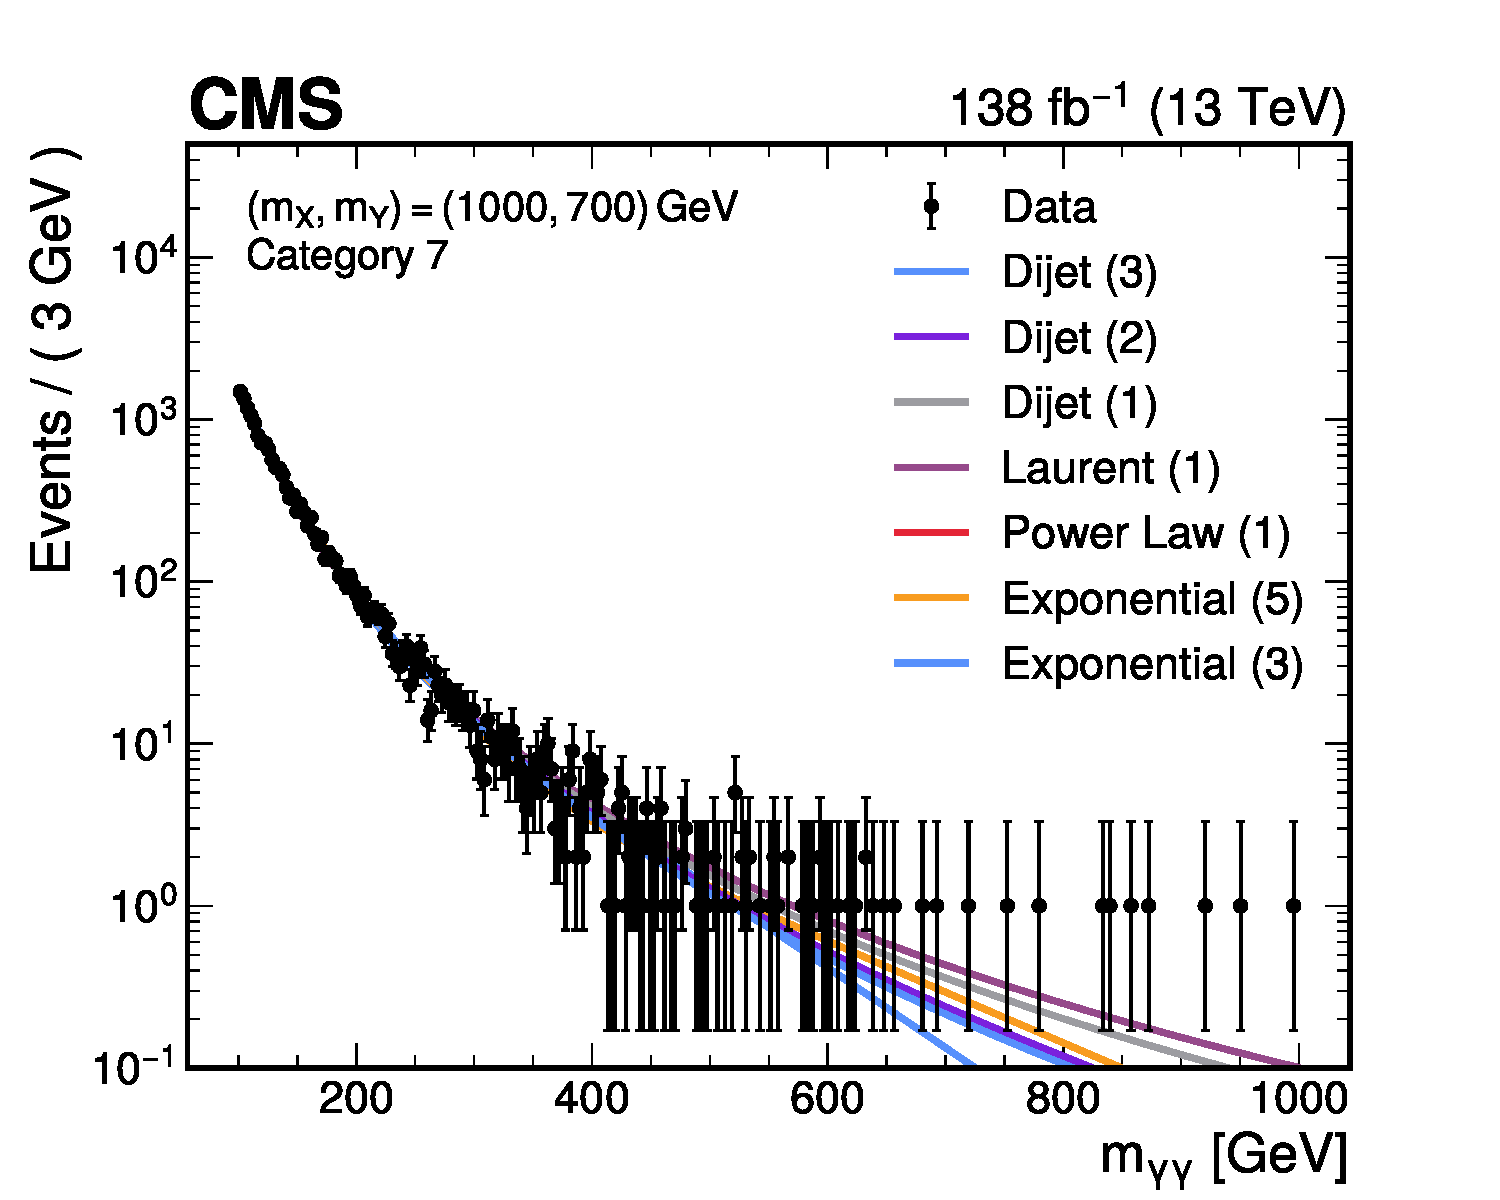
\includegraphics[width=.49\linewidth]{Figures/Dihiggs/background/envelope/y_gg_high_mass/bkgmodel_pdfs_ggttresmx1000my700cat7_log.pdf}
  \caption[Envelope Construction for $(\mX,\mY)=(1000,700)$\GeV in the \XYggHtt Search]{Envelope construction for the $(\mX,\mY)=(1000,700)$\GeV mass point in the \XYggHtt search. Shown is the \mgg distribution in data for a category consisting of the events passing preselection but not passing the pNN selection. The functions entering the envelope are indicated in the legend and their fits to the \mgg distributions are shown in the plots. The same plot is shown with a linear (left) and log (right) y-scale.}\label{fig:envelope_examples_ygg_high_cat7}
\end{figure}

\subsection{Resonant Background from Electron Misidentification}\label{sec:dy_bkg_modelling}
In the low-mass \XYggHtt search, there is an additional background originating from Drell-Yan ($\Pp\Pp\to\PZ$) where the \PZ boson decays to a pair of electrons which are both misidentified as photons, and where associated jets are misidentified as tau leptons. A smaller contribution also arises from diboson ($\Pp\Pp \to \PZ\PZ / \PW\PW / \PZ\PW$) events, where a \PZ boson decays to a pair of electrons which are both misidentified as photons, and the other vector boson decays to tau lepton(s) which are then selected. If both electrons from a \Zee decay are selected to form a diphoton candidate, this would result in a peak in the \mgg distribution at the \PZ boson mass. The modelling of this background is therefore crucial to avoid the reporting of a false signal. Given that this background primarily arises from Drell-Yan (DY) events, it is referred to as the DY background.

Initially, simulated DY and diboson events were studied as way to model the DY background. However, the statistics were too small to provide a reliable estimate of the expected number of events in the analysis categories. Therefore, a data-driven approach was instead developed, using an ABCD method with control regions based upon the pNN selection and the CSEV and pixel veto (\cref{sec:eg_id}). At a given mass point, the regions defined by the analysis categories are denoted $D_i$. The objective of the ABCD method is to create a model of the resonant background (from $e\to\gamma$ misidentification) in each $D_i$ region. 

Each $D_i$ region has a corresponding $B_i$ region that has the same pNN selection but uses a dielectron trigger and inverts the CSEV and pixel veto (inverted selection). By inverting the vetoes, electrons from \Zee decays are likely to be reconstructed and selected as photon candidates, thereby creating a region where the \mgg peak from the \Zee decay is dominant, which is shown in \cref{fig:dy_cr_examples} (top-right) for the $D_0$ region for the $(\mX,\mY)=(650,95)$\GeV mass point. In both $D_i$ and $B_i$, the \mgg variable is constructed using information from the ECAL only. Given that the shower shape of electrons and photons is similar, and that the selection on kinematic variables is the same between regions $B_i$ and $D_i$, the shape of the \mgg peak is expected to be the same in both regions. Therefore, the $B_i$ region is used to derive the shape of the DY background in region $D_i$.

To determine the rate of the DY background in $D_i$, the extracted rate from $B_i$ is multiplied by a transfer factor that is constrained by regions $A$ and $C$. Region $C$ is defined by the normal preselection and an inversion of the pNN selection, i.e.\ contains events that do not pass the pNN selection for any of the analysis categories. Region $A$ has the same pNN selection but uses a dielectron trigger and inverts the CSEV and pixel veto. Examples of the \mgg distributions in these regions are also shown for the $(\mX,\mY)=(650,95)$\GeV mass point in \cref{fig:dy_cr_examples} (left). 

\begin{figure}
  \centering
  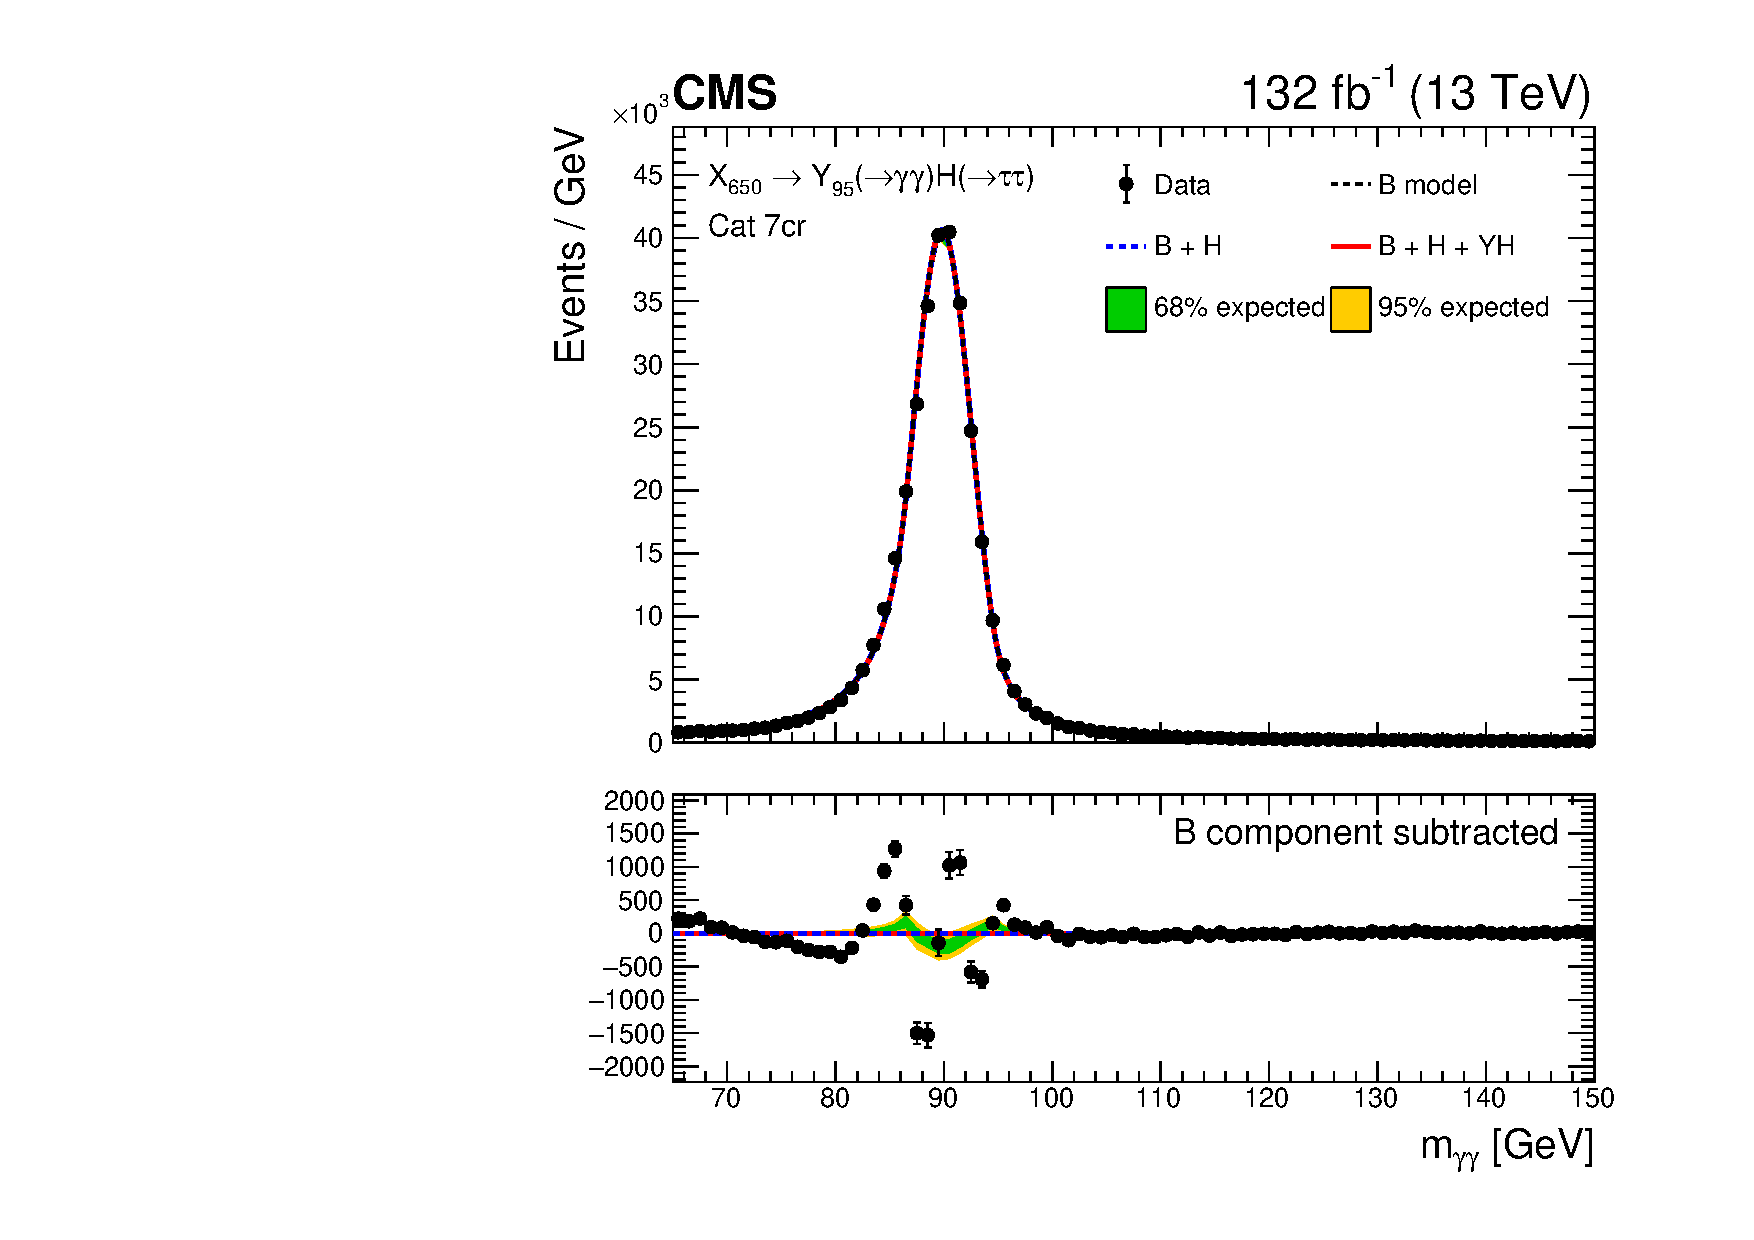
\includegraphics[width=.45\linewidth]{Figures/Dihiggs/results/sb_models/y_gg_low_mass_mx650my95/ARCGL_Y_gg_Low_Mass_mx650my100mh95_ggttresmx650my100cat7cr_CMS_hgg_mass_nbins85_paper.pdf}
  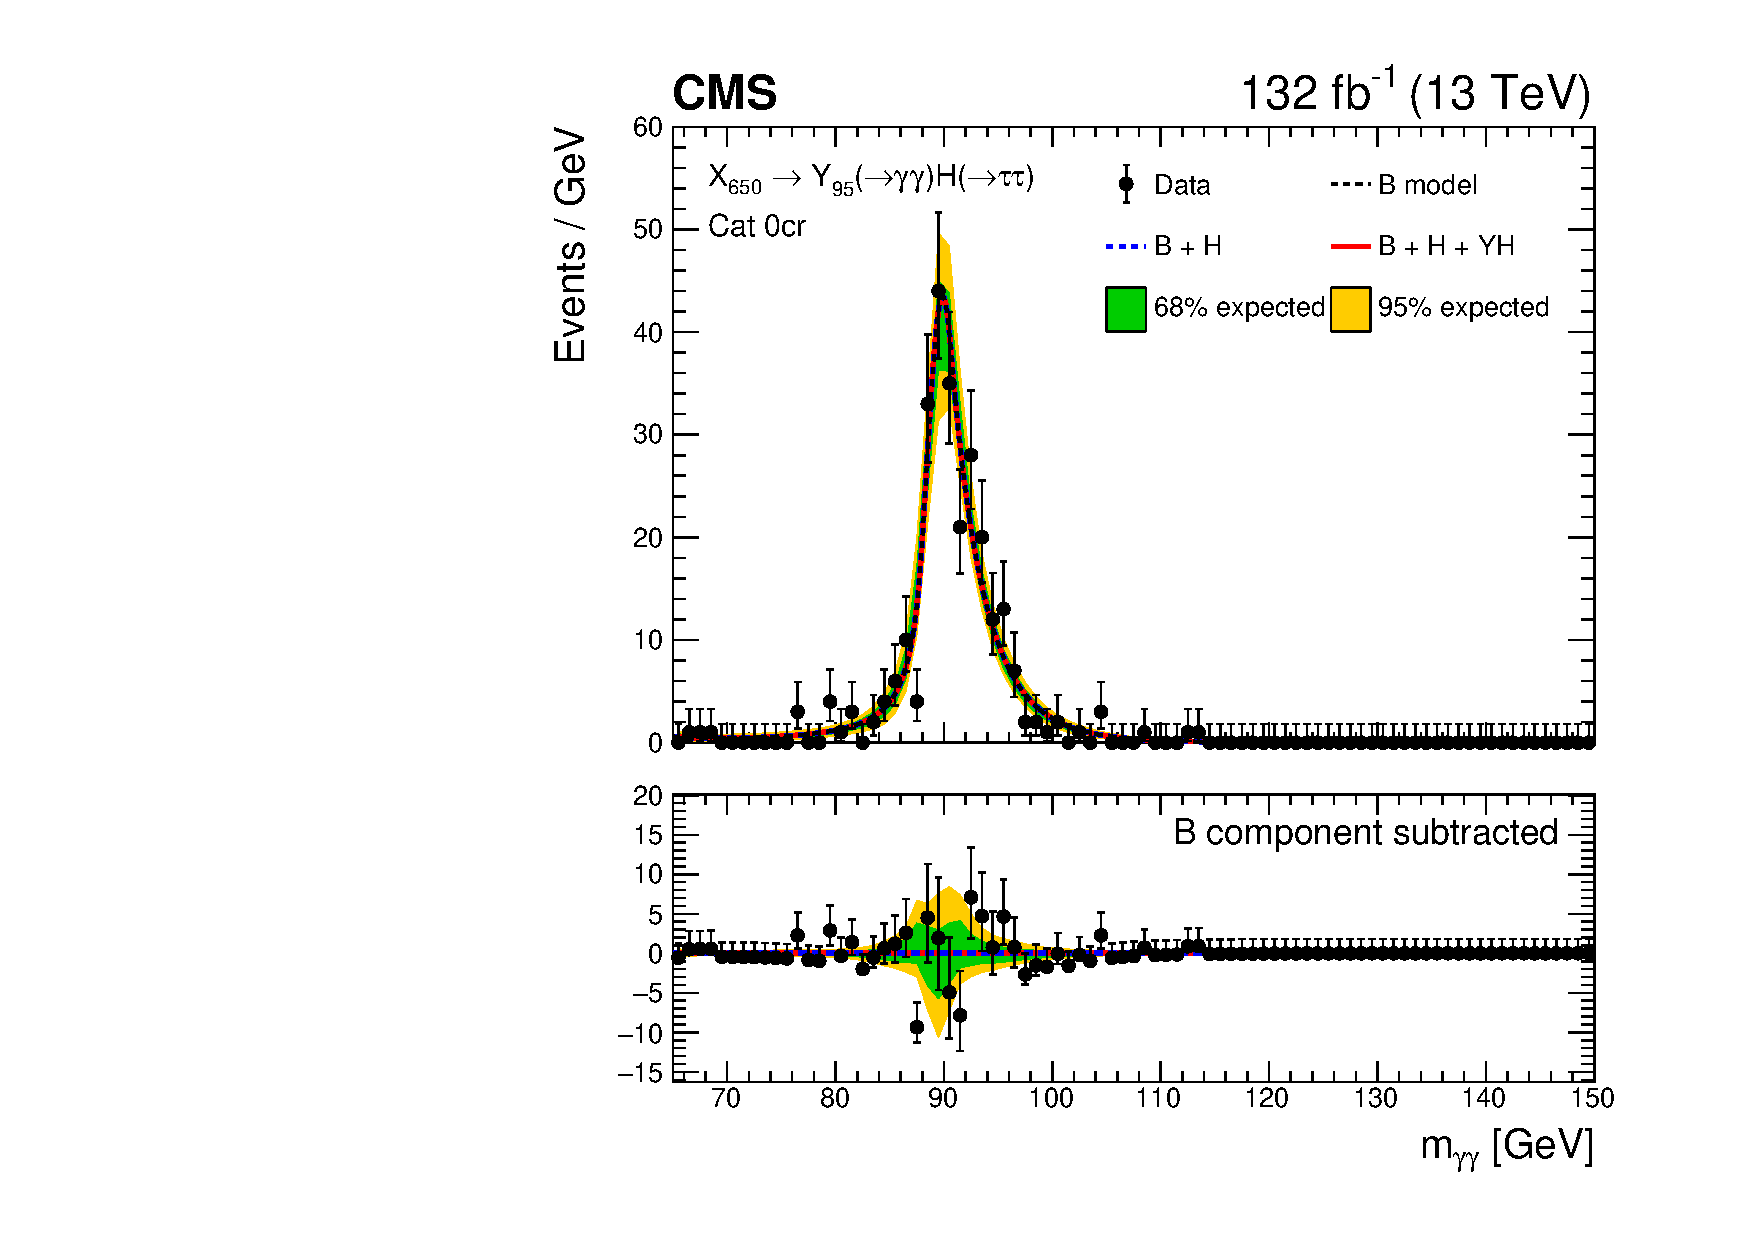
\includegraphics[width=.45\linewidth]{Figures/Dihiggs/results/sb_models/y_gg_low_mass_mx650my95/ARCGL_Y_gg_Low_Mass_mx650my100mh95_ggttresmx650my100cat0cr_CMS_hgg_mass_nbins85_paper.pdf}
  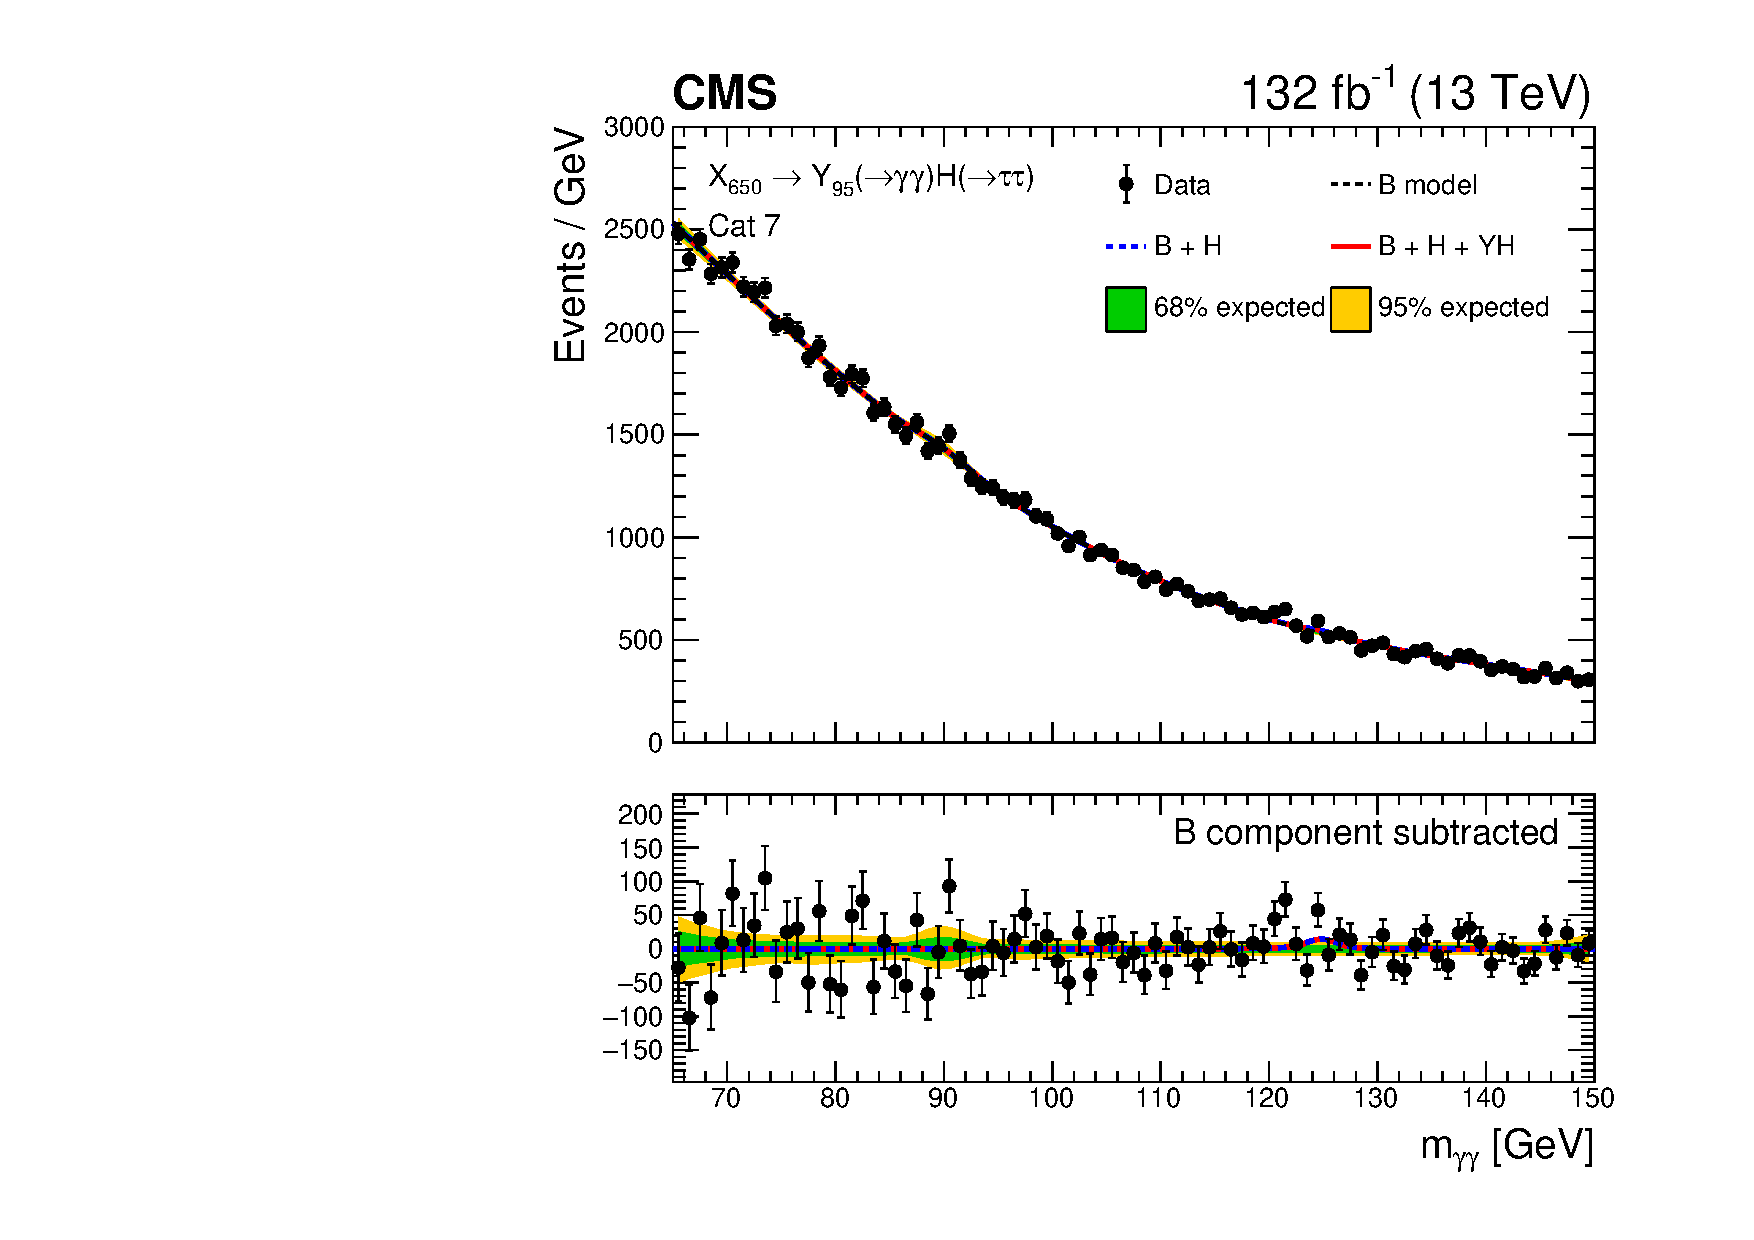
\includegraphics[width=.45\linewidth]{Figures/Dihiggs/results/sb_models/y_gg_low_mass_mx650my95/ARCGL_Y_gg_Low_Mass_mx650my100mh95_ggttresmx650my100cat7_CMS_hgg_mass_nbins85_paper.pdf}
  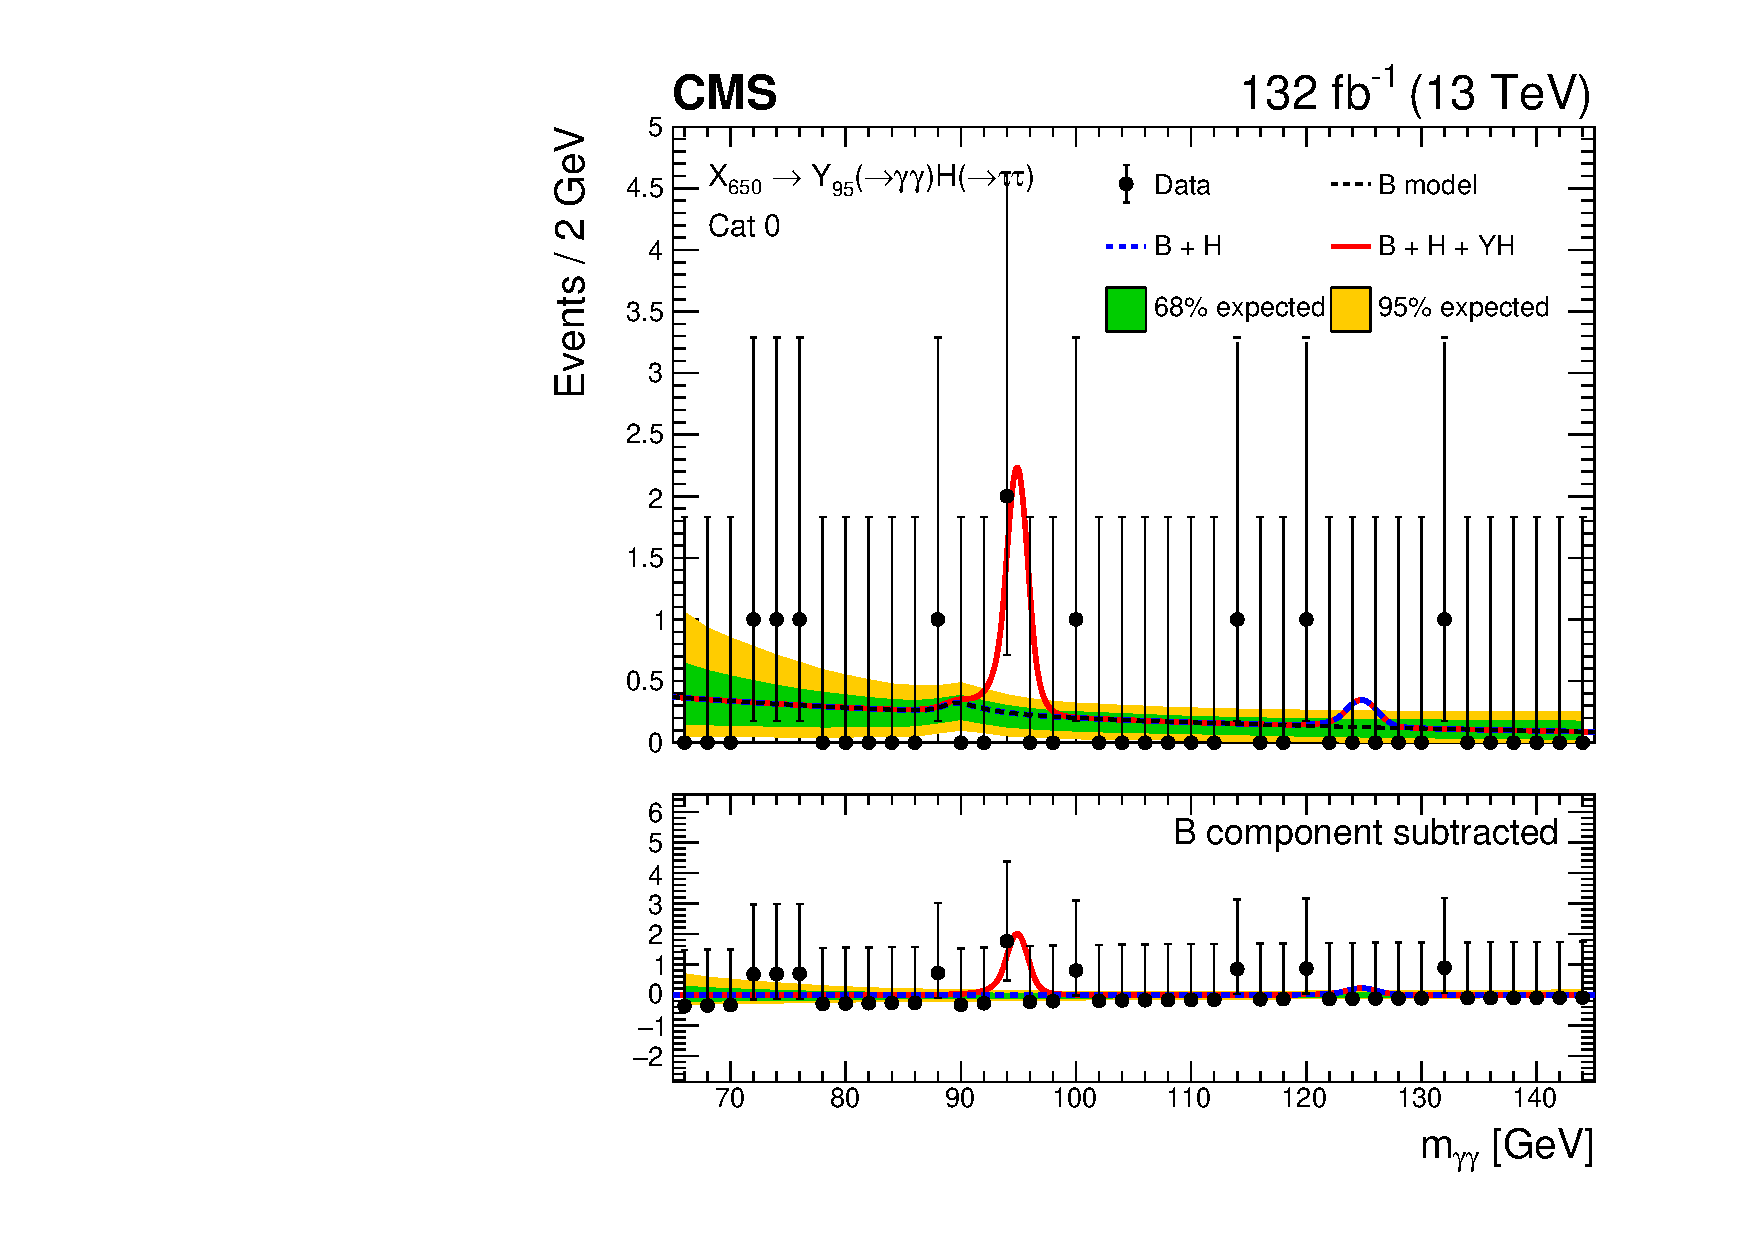
\includegraphics[width=.45\linewidth]{Figures/Dihiggs/results/sb_models/y_gg_low_mass_mx650my95/ARCGL_Y_gg_Low_Mass_mx650my100mh95_ggttresmx650my100cat0_CMS_hgg_mass_nbins40_paper.pdf}
  \caption[Distributions of \mgg in Different Regions of the DY ABCD Method]{Distributions of $\mgg$ in data in regions $A$ (top-left), $B_0$ (top-right), $C$ (bottom-left), and $D_0$ (bottom-right) for the low-mass \XYggHtt search and for $(\mX, \mY) = (650, 95)$\GeV. A signal-plus-background fit (red) is performed with data (black points). The nonresonant background is modelled following the methods described in \cref{sec:non_res_bkg_modelling}. The DY background is described by a DCB or a Gaussian function depending on goodness-of-fit tests. In this example, DCB functions are used in all regions where the shape parameters are shared between regions $A$ and $C$, and a separate set of parameters are shared between regions $B_0$ and $D_0$. The one (green) standard deviation and two (yellow) standard deviation bands show the uncertainties in the nonresonant + DY background component of the model (black dashed line).}\label{fig:dy_cr_examples}
\end{figure}
  
In every region, there is a nonresonant background that is treated in the same way as described in \cref{sec:non_res_bkg_modelling}. The ABCD method is then implemented by adding a DY process to every region where the expected number of events in region $D$ is given by:
\begin{equation}
  \lambda_D = \lambda_B \times \frac{\lambda_C}{\lambda_A}
\end{equation} 
where $\lambda_j$ is the number of events in region $j \in \{A,B,C\}$, where these values are left as free parameters in the fit to data. The function chosen to parameterize the shape of the DY background is the same for each pairing of $D_i$ and $B_i$, and can be a Gaussian or a DCB. At first, a Gaussian function is fit to the \mgg distribution in region $B_i$, and a goodness-of-fit test is performed. If the p-value is greater than 0.01, then a Gaussian function is used, otherwise a DCB function is used. In the final fit to data, the shape parameters, $\vec{\Psi}_i$, for the function are the same in regions $D_i$ and $B_i$ for a given $i$, but change across different $i$, to account for how the pNN selection may influence the \mgg shape. The shape parameters are also left to float in the final fit to data. 

This ABCD method assumes that the shape of the pNN score is the same regardless of whether the normal preselection or inverted selection is used. In other words, the variables used to define the ABCD regions are uncorrelated. This was tested in simulated DY and diboson events where the reconstructed photons were matched to electrons from \Zee decays at the generator level. The shapes of the pNN score for the $\mY=90$\GeV and $\mX=300$, 500, 800 and 1000\GeV mass points, for the normal preselection and inverted selected are shown in \cref{fig:dy_correlation_check}. Within the statistical uncertainties, the two distributions are compatible, and the same is found for other values of $\mX$ at $\mY=90$\GeV.

\begin{figure}
  \centering
  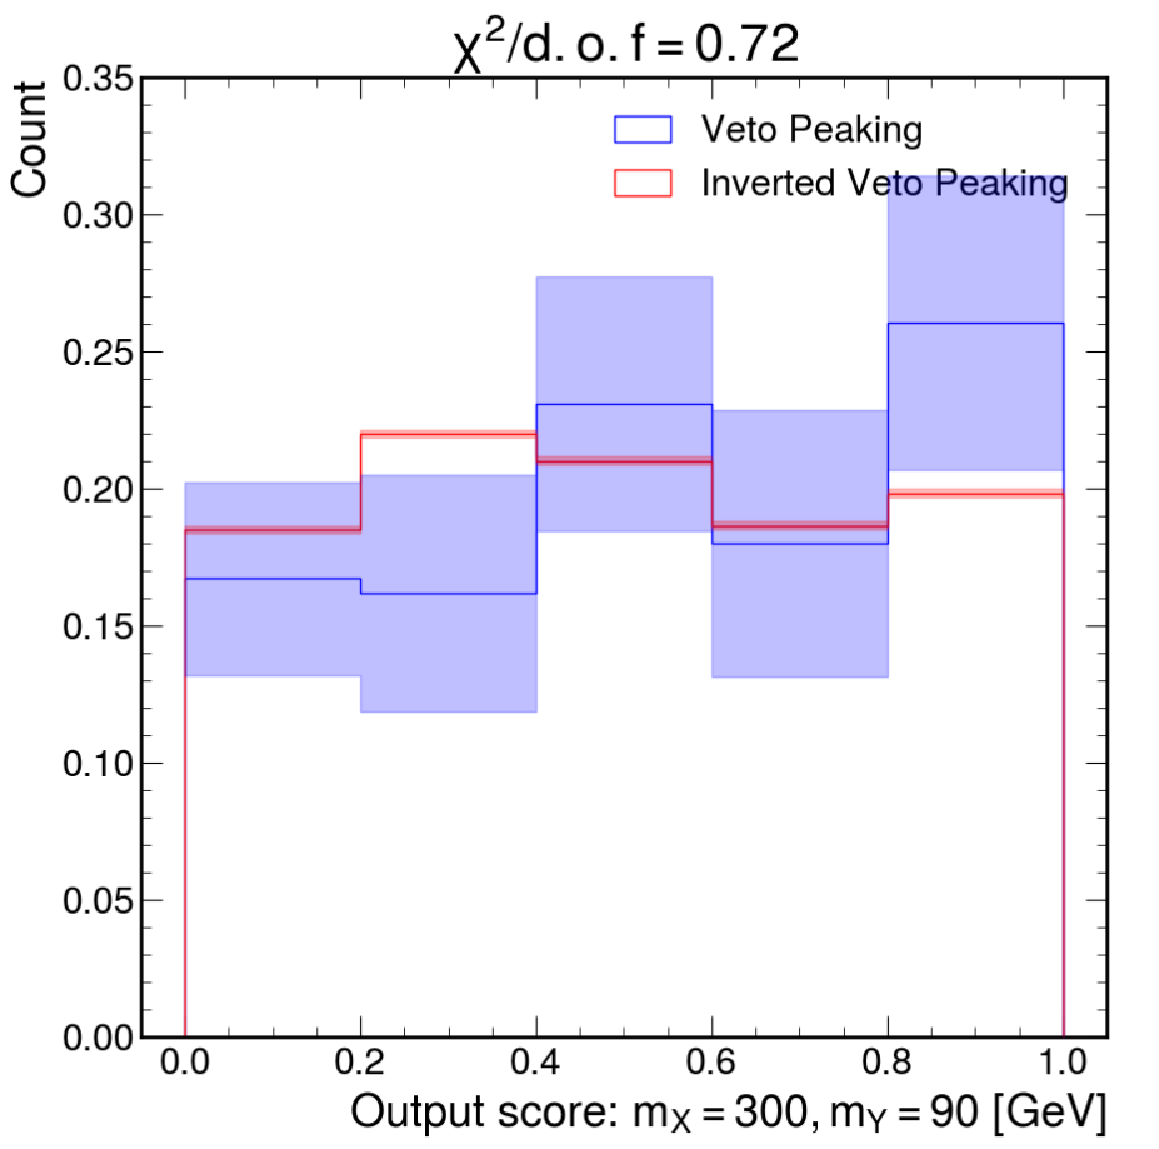
\includegraphics[width=0.45\textwidth]{Figures/Dihiggs/background/dy/output_score_300.pdf}\hspace{0.05\textwidth}
  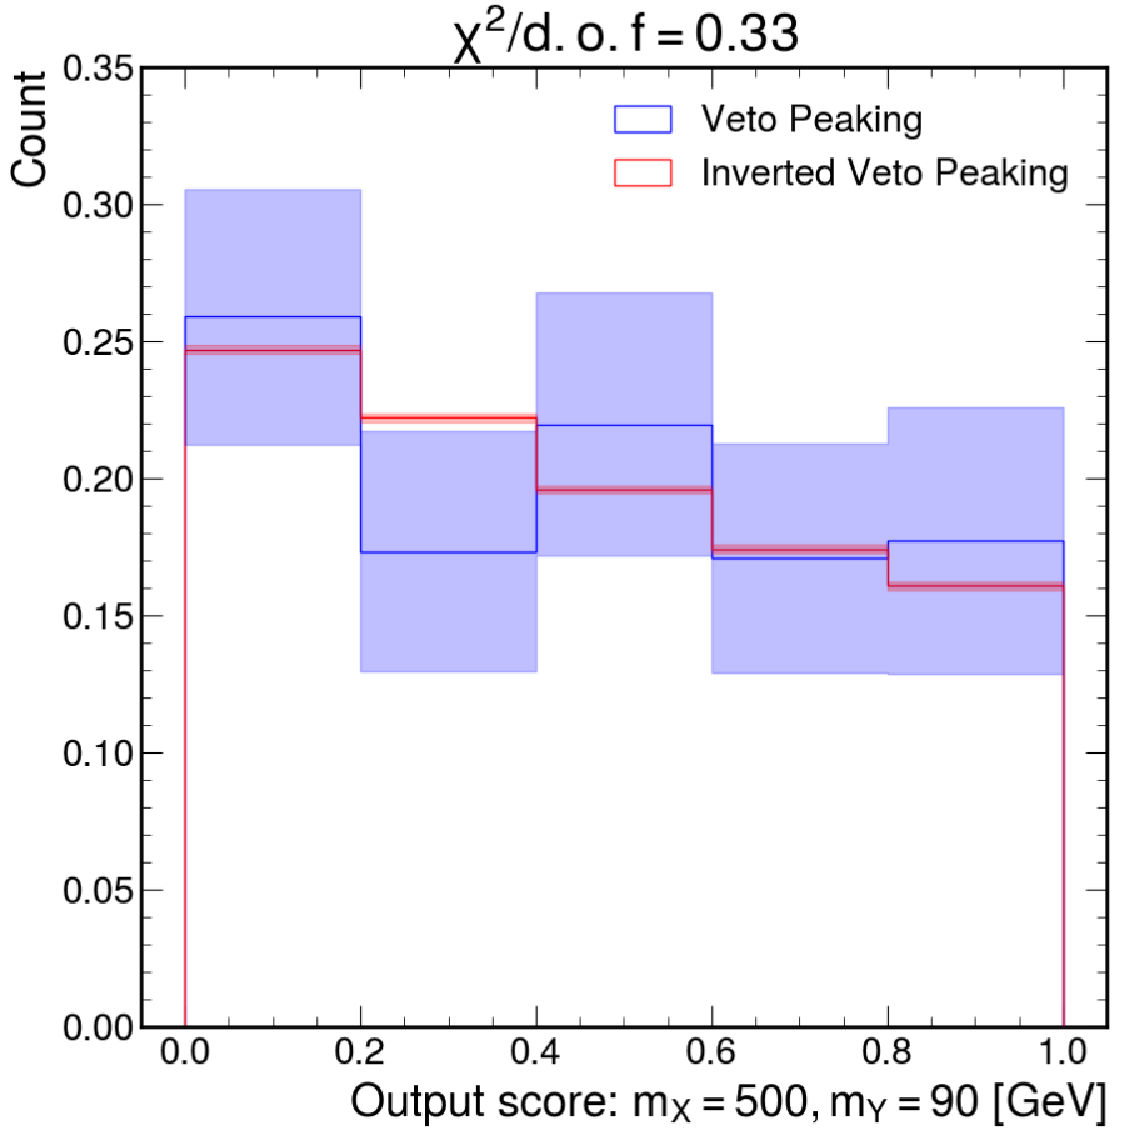
\includegraphics[width=0.45\textwidth]{Figures/Dihiggs/background/dy/output_score_500.pdf}\vspace{0.05\textwidth}
  \includegraphics[width=0.45\textwidth]{Figures/Dihiggs/background/dy/output_score_800.pdf}\hspace{0.05\textwidth}
  \includegraphics[width=0.45\textwidth]{Figures/Dihiggs/background/dy/output_score_1000.pdf}
  \caption[Correlation Check for the DY ABCD Method]{Distribution of the transformed pNN output score, $\tilde{f}(\vec{x};\mX,\mY)$, in the low-mass \XYggHtt search for $\mY=90$\GeV and $\mX=300$ (top-left), 500 (top-right), 800 (bottom-left) and 1000\GeV (bottom-right). The distributions are made from simulated DY and diboson events where the reconstructed photons are  matched to electrons from \Zee decays at the generator level, and with the normal preselection (blue) applied, or with the inverted selection (red) applied. The statistical uncertainty is shown by the shaded bands and the compatibility of the two distributions are tested with a $\chi^2$ statistic.}\label{fig:dy_correlation_check}
\end{figure}

The expected number of DY events (yield) in the $D$ regions extracted from a background-only maximum likelihood fit to data using this ABCD method are shown in \cref{fig:dy_expected_events}. The yields in $D_0$ are shown as a function of \mX for $\mY = 90$ and 100\GeV, and are found to range between about 0.03 and 0.4 with an upwards trend in \mX. The numbers are also shown in regions $D_0$ to $D_3$ for the $(\mX, \mY)=(650,100)$\GeV and $(\mX, \mY) = (325,100)\GeV$ where yields remain below 0.4, which is also the case for all other mass points. Given the small expected number of events, the impact on the final results is expected to be small. This is discussed further in \cref{sec:ggtt_results}.

\begin{figure}
  \centering
  \includegraphics[width=0.6\textwidth]{Figures/Dihiggs/background/dy/dy_yield_vs_mx.pdf}
  \includegraphics[width=0.6\textwidth]{Figures/Dihiggs/background/dy/dy_yield_vs_category.pdf}
  \caption[Expected DY Events Extracted Using ABCD Method]{Expected number of DY events (yields) in regions $D_i$ ($\lambda_D$) extracted from a background-only maximum likelihood fit to data. On the top, the yields are shown for region $D_0$ as a function of \mX for $\mY = 90$ and 100\GeV. On the bottom, the yields are shown for regions $D_i$ where $i$ denotes the category, for the $(\mX, \mY)=(650,100)$\GeV and $(\mX, \mY) = (325,100)\GeV$ mass points. The error bars indicate the statistical uncertainty in the yields extracted from the fit.}\label{fig:dy_expected_events}
\end{figure}